% Document class for LME theses: lmedoc
% %LANGUAGE
% %CONFIG
%    The option "german" uses german.sty
%    For english papers, use the "english" option
% Possible types of theses:
% bt - Bachelor's thesis
% mt - Master's thesis
% diss - Dissertation
% sa - Student thesis
% fp - Forschungspraktikum
% pa - Projektarbeit
%\documentclass[german,bt]{lmedoc/lmedoc}
\documentclass[english,mt]{lmedoc/lmedoc}


%%%%%%%%%%%%%%%%%%
% pdflatex and lualatex are supported
% ++ "Umlaut" support
%    The package "inputenc" can be used to write Umlaute or the german double s
%    directly. You need to use the correct encoding, e.g. latin1.
\usepackage{iftex}
\ifPDFTeX
  \usepackage[utf8]{inputenc}
  \usepackage[T1]{fontenc}
  \usepackage{lmodern}
\else
  \ifXeTeX
     \usepackage{fontspec}
  \else 
     \usepackage{luatextra}
  \fi
\fi

%Load additional packages
\usepackage{lmedoc/packages}
% TikZ libraries used by the methodology pipeline figure
\usetikzlibrary{positioning,arrows.meta,shapes.geometric}
% \FloatBarrier for keeping figures within their section
\usepackage{placeins}
% put in this file your abbreviations
% Abbreviations / acronyms used in the thesis.
% Usage in text: \gls{ct} (first use expands), \gls{ldct}, \glspl{cnn} (plural)

\newabbreviation{ct}{CT}{Computed Tomography}
\newabbreviation{ldct}{LDCT}{Low-Dose Computed Tomography}
\newabbreviation{fbp}{FBP}{Filtered Back-Projection}
\newabbreviation{cnn}{CNN}{Convolutional Neural Network}
\newabbreviation{unet}{U-Net}{U-shaped Encoder--Decoder Network}
\newabbreviation{redcnn}{RED-CNN}{Residual Encoder--Decoder CNN}
\newabbreviation{dncnn}{DnCNN}{Denoising Convolutional Neural Network}
\newabbreviation{bm3d}{BM3D}{Block-Matching and 3D Filtering}
\newabbreviation{psnr}{PSNR}{Peak Signal-to-Noise Ratio}
\newabbreviation{ssim}{SSIM}{Structural Similarity Index}
\newabbreviation{lpips}{LPIPS}{Learned Perceptual Image Patch Similarity}
\newabbreviation{mae}{MAE}{Mean Absolute Error}
\newabbreviation{mse}{MSE}{Mean Squared Error}
\newabbreviation{roi}{ROI}{Region of Interest}
\newabbreviation{hu}{HU}{Hounsfield Unit}
\newabbreviation{mar}{MAR}{Metal Artifact Reduction}
\newabbreviation{dl}{DL}{Deep Learning}
\newabbreviation{gpu}{GPU}{Graphics Processing Unit}
\newabbreviation{lodopab}{LoDoPaB}{Low-Dose Parallel-Beam CT}
\newabbreviation{lme}{LME}{Pattern Recognition Lab (Lehrstuhl f\"ur Mustererkennung)}
%%%%%%%%%%%%%%%%%%%%%%%%%%%%

% supress messages because of underful hbox, this is not a problem
\hbadness=10000



% some useful commands
\makeatletter % let's define a single dot
\DeclareRobustCommand\onedot{\futurelet\@let@token\@onedot}
\newcommand{\@onedot}{\ifx\@let@token.\else.\null\fi\xspace}
% float pages: pin content to top instead of vertically centring
\setlength\@fptop{0pt}
\makeatother



% Sets the bib file

\addbibresource{literature.bib}

% When writing a large document, it is sometimes useful to work on selected sections of the document.
% Use this command to only build the document partially. Speeds up the developement cycle.
% For the final product, this has to be commented out.
%\includeonly{introduction,appendix,foo,bar}


\pagenumbering{roman}

\begin{document}
\clearpage
% %CONFIG
% This is for students' theses
  \begin{deckblatt}
    \Titel{A Cascaded Encoder-Decoder for CT Image Restoration} % Title
    \Name{Shiblu} % Last name
    \Vorname{Mohammad} % Given name
    \Geburtsort{Dhaka} % Place of birth
    \Geburtsdatum{02.07.1996} % Date of birth
    \Betreuer{Yipeng Sun, Prof. Dr. Andreas Maier} % Advisor
    \Start{01.11.2025} % Start of thesis
    \Ende{04.05.2026} % End of thesis
    %\ZweitInstitut{ZweitInstitut} % Cooperation partner
  \end{deckblatt}


\cleardoublepage
% Only necessary for thesis

Ich versichere, dass ich die Arbeit ohne fremde Hilfe und ohne Benutzung
anderer als der angegebenen Quellen angefertigt habe und dass die Arbeit
in gleicher oder "ahnlicher Form noch keiner anderen Pr"ufungsbeh"orde
vorgelegen hat und von dieser als Teil einer Pr"ufungsleistung
angenommen wurde. Alle Ausf"uhrungen, die w"ortlich oder sinngem"a"s
"ubernommen wurden, sind als solche gekennzeichnet.

Die Richtlinien des Lehrstuhls für Examensarbeiten habe ich gelesen und anerkannt,
insbesondere die Regelung des Nutzungsrechts in Punkt 2.5

\vspace*{2cm}  % medium space
\noindent
\begin{tabular}{p{0.5\textwidth} p{0.5\textwidth}}
Erlangen, den ........ &  \centering Unterschrift
\end{tabular}


\cleardoublepage


\begin{center}
\bfseries
% Abstract in German (max 0.5 pages, required by LME guidelines §1.3)
{\selectlanguage{german}"Ubersicht}
\normalfont
\end{center}

{\selectlanguage{german}%
CT-Bilder in der klinischen Praxis leiden häufig unter zusammengesetzter Degradation durch Poisson-Rauschen sowie Bewegungs-, Ring- und Metallartefakte, während die meisten Restaurationsverfahren diese Effekte getrennt behandeln. Diese Arbeit untersucht, ob kaskadierte Encoder--Decoder-Netzwerke die CT-Bildrestauration unter solcher zusammengesetzter Korruption verbessern, indem ein physikalisch motiviertes Korruptionsprotokoll im Sinogrammbereich für LoDoPaB-CT entwickelt und drei zweistufige Varianten verglichen werden: unabhängiges stufenweises Training, End-to-End-Training und eine Residualformulierung.

Ein großes einstufiges U-Net erreicht unter der vorgeschlagenen Korruption 36.11 dB PSNR. Bei gleicher kleiner Kapazität pro Stufe bringt eine zusätzliche zweite Stufe nur begrenzte Verbesserungen gegenüber der kleinen einstufigen Basisvariante (35.39 dB), nämlich +0.15 bis +0.72 dB. Die beste kleine Kaskade, basierend auf Residualvorhersage mit Hann- und Shepp--Logan-gefilterten FBP-Eingaben, erreicht ebenfalls 36.11 dB, übertrifft die große einstufige Referenz jedoch nicht. Die Gradientenanalyse zeigt eine Abschwächung des Lernsignals der zweiten Stufe während der Konvergenz von Stufe 1, was darauf hindeutet, dass die für Stufe 2 verfügbare Information und nicht allein die Tiefe den Hauptengpass bildet.
}

\vspace{1.5cm}

\begin{center}
\bfseries
% Abstract in English (max 0.5 pages)
{\selectlanguage{english}Abstract}
\normalfont
\end{center}

{\selectlanguage{english}%
CT images in clinical practice often suffer from compound degradation caused by Poisson noise together with motion, ring, and metal artifacts, yet most restoration methods treat these effects separately. This thesis investigates whether cascaded encoder--decoder networks improve CT image restoration under such compound corruption by developing a physics-informed sinogram-domain corruption protocol for LoDoPaB-CT and comparing three two-stage formulations: independent-stage, end-to-end, and residual.

A single large U-Net reaches 36.11 dB PSNR under the proposed corruption. At matched small per-stage capacity, adding a second stage yields only limited gains over the small single-stage baseline (35.39 dB), ranging from +0.15 to +0.72 dB. The best small cascade, using residual prediction with Hann- and Shepp--Logan-filtered FBP inputs, matches the large single-stage reference at 36.11 dB without exceeding it. Gradient analysis shows attenuation of the Stage-2 learning signal as Stage-1 converges, indicating that information available to the second stage, rather than depth alone, is the main bottleneck.}


\cleardoublepage

% Notation table (required: all math symbols defined once, LME §1.6.4)
% Notation table — required by LME guidelines (§1.6.4):
% all mathematical symbols used in the thesis must be defined exactly once.

\chapter*{Notation}
\addcontentsline{toc}{chapter}{Notation}

\begin{tabular}{p{0.18\textwidth} p{0.75\textwidth}}
    \toprule
    \textbf{Symbol} & \textbf{Meaning} \\
    \midrule
    $\boldsymbol{x}$        & Ground-truth CT image (2D slice, linearised to vector when needed) \\
    $\boldsymbol{\hat{x}}$  & Network-predicted (restored) CT image \\
    $\boldsymbol{s}$        & Clean sinogram (Radon transform of $\boldsymbol{x}$) \\
    $\boldsymbol{\tilde{s}}$& Corrupted sinogram after artifact injection \\
    $\boldsymbol{y}$        & Input to the restoration network (FBP of $\boldsymbol{\tilde{s}}$) \\
    $\mu(\boldsymbol{r})$   & Linear attenuation coefficient at position $\boldsymbol{r}$ \\
    $I_0$                   & Incident photon count (controls dose level) \\
    $N$                     & Measured photon count; $N \sim \mathrm{Poisson}(I_0 e^{-s})$ \\
    $\mathcal{R}$           & Radon transform operator \\
    $\mathcal{R}^{-1}$      & Filtered back-projection (FBP) operator \\
    $\boldsymbol{\theta}$   & Learnable parameters of a network \\
    $\mathcal{L}$           & Training loss (L1 / MAE unless stated otherwise) \\
    $f_k(\cdot;\boldsymbol{\theta}_k)$ & The $k$-th stage network \\
    $\boldsymbol{x}_k$      & Output of the $k$-th cascade stage \\
    $\|\cdot\|_1$           & $\ell^1$ norm (element-wise mean absolute value in loss context) \\
    \bottomrule
\end{tabular}

\cleardoublepage

\tableofcontents

\cleardoublepage \pagenumbering{arabic}

\chapter{Introduction}
\label{chap:introduction}

\section{Background and Motivation}
\label{sec:intro_motivation}

Computed tomography (\gls{ct}) is one of the most widely used imaging modalities in modern medicine. By acquiring X-ray attenuation measurements from numerous projection angles and reconstructing them into cross-sectional images, CT enables non-invasive visualization of internal anatomy with high diagnostic accuracy. This capability supports the detection of pulmonary nodules, the characterization of cardiovascular lesions, the staging of oncologic disease, and the evaluation of trauma without the need for surgical intervention \cite{Sadia2024, Komolafe2024}. Due to its substantial clinical utility, the global volume of CT examinations has increased steadily over the past two decades.

This growth, however, is accompanied by an unavoidable cost: exposure to ionizing radiation. Each CT scan delivers an X-ray dose to the patient, and cumulative exposure is associated with a small but well-documented risk of stochastic biological harm, including radiation-induced malignancy \cite{Sadia2024, AAPM2016}. In particular, a large retrospective cohort study reported an increased risk of leukemia and brain tumors in children who underwent repeated CT examinations~\cite{Pearce2012}. Because the radiation dose of the patient scales directly with the current of the X-ray tube, the most straightforward strategy for reducing the dose is to lower the current of the tube, which forms the basis of \gls{ldct}. However, this approach introduces a substantial trade-off. As fewer photons reach the detector, the measured sinogram becomes increasingly dominated by quantum noise governed by Poisson statistics. When reconstructed using \gls{fbp}, which remains the standard analytical method in clinical practice, this noise propagates into the image domain as low-frequency granular noise, streak artifacts, and reduced soft-tissue contrast~\cite{Leuschner2021}. As a result, image quality can be diagnostically compromised, thus limiting the extent to which the radiation dose can be reduced in routine practice~\cite{AAPM2016}.

Noise is not the only source of image degradation in CT. In routine clinical imaging, CT scans are often affected by multiple co-occurring physical artifacts that arise from the acquisition process itself rather than from photon statistics alone~\cite{Boas2012}. Even minor patient motion during scanning, such as breathing, swallowing, or involuntary cardiac movement, can introduce inconsistencies across projections, leading to blurring and ghosting in the reconstructed image, particularly around moving structures \cite{LuMackie2002, Lu2005}. Detector miscalibration or damage to individual detector elements may further produce ring artifacts, which appear as concentric circular bands centered on the axis of rotation and can obscure subtle lesions near the center of the field of view \cite{Sijbers2004, Prell2009}. In addition, metallic implants, including hip prostheses, dental fillings, pacemaker leads, and surgical clips, cause extreme attenuation that leads to photon starvation along affected projection paths and generate pronounced bright and dark streak artifacts, often rendering substantial image regions uninterpretable \cite{ZhangYu2018, Gjesteby2016}. Importantly, these degradations rarely occur in isolation. For example, a low dose postoperative patient may simultaneously present with Poisson noise, ring artifacts caused by detector drift, and metal artifacts associated with the implant. Nevertheless, most deep learning studies continue to address these sources of degradation independently rather than as interacting components of a single clinical imaging problem \cite{Liang2025}.

During the past three decades, substantial algorithmic effort has been devoted to recovering diagnostic image quality from degraded CT data. Classical approaches include hand-crafted image-domain post-processing filters, total variation minimization, dictionary-learning-based denoising, and non-local means methods \cite{Sadia2024, Tian2020}. Among these, Block-Matching and 3D Filtering (\gls{bm3d}) \cite{Dabov2007} occupies a distinctive position because it exploits non-local self-similarity to achieve state-of-the-art performance for additive Gaussian noise without requiring training data, making it a natural benchmark against which learned methods are often evaluated. On the reconstruction side, iterative methods that incorporate statistical noise models and anatomical regularization priors, most notably the constrained total-variation minimization framework of Sidky and Pan \cite{SidkyPan2008}, can outperform FBP in low-dose settings, although their computational cost remains a significant obstacle to routine clinical use \cite{Beister2012}.

Supervised deep learning has emerged as the dominant paradigm in CT image restoration. Convolutional encoder--decoder architectures, popularized in biomedical imaging by the U-Net~\cite{Ronneberger2015}, have been widely adapted for CT restoration tasks. Trained on paired degraded and reference images, these models learn an end-to-end mapping from corrupted input to high-quality output. A landmark example is the Residual Encoder--Decoder CNN (RED-CNN) \cite{Chen2017}, which introduced skip connections between the corresponding encoder and decoder layers to preserve fine structural detail during compression. In parallel, DnCNN \cite{Zhang2017} showed that learning residual noise, rather than directly predicting clean image, can accelerate convergence and improve denoising performance, following a strategy inspired by residual learning in ResNet-style architectures \cite{He2016}. A related line of work further demonstrated that the same encoder--decoder principle can be applied to the output of an analytic reconstructor in general inverse problems \cite{Jin2017}, while adversarial and perceptual losses were later introduced to mitigate the over smoothing often associated with pure $\ell^{2}$ optimization \cite{Yang2018WGAN}. These ideas have since been combined and extended in numerous forms, including attention-based architectures \cite{Komolafe2024, Zhang2023}, dual-domain methods that jointly process sinogram and image data~\cite{Wang2020, Zhang2022, Lin2019DuDoNet}, and model-based unrolled networks that explicitly incorporate the forward operator into the reconstruction architecture~\cite{Aggarwal2019MoDL, Hammernik2018VarNet}. Recent benchmarking studies have also shown that the performance reported of these methods can be highly sensitive to the corruption protocol and evaluation data set, underscoring the need for reproducible and physics-consistent test conditions~\cite{Kiss2024}.

Despite this rapid progress, two important questions remain insufficiently explored. First, most existing methods are designed and evaluated for a single isolated degradation type, most commonly simulated Poisson noise at a prescribed dose level, while implicitly assuming the absence of other artifact sources. Although this simplification facilitates benchmarking, it creates a clear mismatch with clinical reality, where multiple degradation mechanisms often coexist within the same scan~\cite{Boas2012, Liang2025}. At present, there is no widely established protocol for jointly simulating this compound corruption distribution in the sinogram domain in a physics-consistent manner. Second, although cascade architectures, in which two or more restoration networks are applied sequentially, are widely used in practice, the question of how the stages should be coupled has received comparatively little systematic study. In particular, it remains unclear whether stages should be trained independently with gradients stopped at stage boundaries, or instead optimized jointly in an end-to-end manner. Similarly, the effect of formulating each stage as a residual corrector rather than a complete restoration module remains poorly understood. These design choices have important implications for gradient propagation, optimization stability, and the extent to which performance can be improved by increasing cascade depth.

This thesis addresses both questions directly by using the LoDoPaB-CT benchmark \cite{Leuschner2021} as its experimental testbed. LoDoPaB-CT is a large-scale, open-access dataset of simulated parallel-beam CT measurements derived from the LIDC/IDRI lung CT database.

\section{Problem Statement}
\label{sec:intro_problem}

This thesis addresses a twofold central challenge. First, it asks how realistic multi-artifact degradation can be simulated faithfully in the sinogram domain so that learned models are exposed to compound corruption distributions that better reflect clinical acquisition. Second, under such a corruption regime, it investigates how architectural depth, specifically the choice between independent-stage, end-to-end, and residual cascade formulations of encoder--decoder networks, influences restoration quality and whether a meaningful performance ceiling exists for additional image-domain stages. These two questions are inherently linked. The effect of cascade depth becomes substantively interesting only when the corruption is sufficiently complex that a single-stage model may be inadequate. Conversely, the value of a realistic corruption protocol can only be assessed through a well-controlled comparison of architectural alternatives in which depth is isolated as the independent variable. Together, these questions define a systematic study of image-domain restoration capacity under physics-informed corruption.

\section{Contributions}
\label{sec:intro_contributions}

This thesis makes two primary contributions:

\begin{enumerate}
    \item \textbf{A physics-informed multi-artifact sinogram corruption protocol.} This thesis develops and validates a modular, reproducible pipeline for the joint simulation of Poisson quantum noise, motion artifacts, ring artifacts, and metal artifacts in the sinogram domain, each at controllable levels of severity. Each component is designed to reflect the physical mechanism that gives rise to the corresponding degradation in real CT acquisition: Poisson photon statistics for quantum noise~\cite{Leuschner2021}, projection inconsistencies induced by motion~\cite{LuMackie2002, Lu2005}, per-detector gain perturbations for ring artifacts~\cite{Sijbers2004, Prell2009}, and high-attenuation insertions with associated photon starvation for metal artifacts~\cite{ZhangYu2018, Gjesteby2016}. The protocol is parameterized to match the parallel-beam geometry and photon statistics of LoDoPaB-CT~\cite{Leuschner2021}, and individual artifact types are sampled independently to generate a compound corruption distribution spanning a broad and clinically plausible range of degradation conditions. Crucially, all corruptions are introduced prior to \gls{fbp} reconstruction, thereby preserving physical consistency in the way they propagate into the image domain.

    \item \textbf{A systematic study of cascade architectures.} Three cascade formulations of a U-Net encoder--decoder are trained and evaluated under the multi-artifact corruption protocol described above: (i)~an \emph{independent-stage} cascade, in which both stages are trained simultaneously but a stop-gradient operator at the stage boundary prevents the Stage-2 loss from reaching Stage-1 parameters, so that each stage is updated only by its own loss; (ii)~an \emph{end-to-end cascade}, in which all stages are optimized jointly under deep supervision~\cite{Lee2015DSN}, with an auxiliary loss applied to each intermediate stage output in addition to the final reconstruction loss, thereby allowing gradients to propagate through the full cascade while providing explicit supervision at every stage; and (iii)~a \emph{residual cascade}, in which each stage predicts an additive correction to the output of the previous stage rather than a full restored image. These three formulations are compared against three baselines --- \gls{bm3d}~\cite{Dabov2007} applied to the FBP reconstruction, a single-stage U-Net~\cite{Ronneberger2015}, and \gls{redcnn}~\cite{Chen2017} --- using \gls{psnr} and \gls{ssim} as the primary evaluation metrics, consistent with current CT benchmarking practice~\cite{Kiss2024}.
\end{enumerate}

The central finding of this thesis is that a single well-designed encoder--decoder network already operates close to the performance ceiling attainable in the image domain under the compound corruption conditions considered. Adding further image-domain cascade stages yields only limited benefit: the naive independent-stage cascade improves on the matched single-stage baseline by just \(+0.15\)\,dB PSNR, while the end-to-end cascade, despite joint training with gradient flow across stages, achieves only \(+0.46\)\,dB and therefore only marginally surpasses the naive variant. These diminishing returns are supported by gradient-norm analysis, which indicates that Stage~2 receives a substantially weaker learning signal once Stage~1 has converged. The residual cascade recovers a small but consistent gain of \(+0.54\)\,dB relative to the naive independent-stage baseline, and, when combined with dual-filter conditioning, is the only cascade configuration that matches the larger single-stage U-Net. Rather than constituting a negative result, this architectural ceiling is scientifically informative: it helps to localize the image-domain information bottleneck and thereby motivates dual-domain approaches that introduce additional information from the sinogram as the logical next step~\cite{Wang2020, Zhang2022}.

\section{Thesis Outline}
\label{sec:intro_outline}

The remainder of this thesis is organized as follows. \Cref{chap:background} provides the theoretical background on CT imaging, the mechanisms of low-dose degradation and physical artifacts, and the deep learning literature relevant to CT image restoration. \Cref{chap:methodology} describes the methodological framework of the thesis, including the physics-informed multi-artifact sinogram corruption protocol (\Cref{chap:corruption}) and the cascaded encoder--decoder architectures, comprising the single-stage baseline, the alternative-filter input scheme, the three coupling strategies, and the common training procedure (\Cref{chap:architectures}). \Cref{chap:experiments} presents the quantitative and qualitative results, together with the gradient analysis and a critical discussion of the findings. Finally, \Cref{chap:conclusion} summarizes the main contributions, discusses the limitations of the study, and outlines directions for future research.
       % Chapter 1: Introduction
\cleardoublepage
\chapter{Background}
\label{chap:background}

This chapter provides the theoretical and methodological background for the remainder of the thesis. It begins by introducing the physics of X-ray CT acquisition and the analytical reconstruction pipeline used throughout this work (\Cref{sec:bg_ct_fundamentals}). It then describes the two main sources of image degradation that the proposed corruption protocol aims to reproduce: photon-counting noise arising at low dose (\Cref{sec:bg_ldct_degradation}) and the deterministic physical artifacts that commonly coexist with it in clinical scans (\Cref{sec:bg_artifacts}). Finally, the chapter reviews the deep learning methods that have come to dominate CT image restoration and situates the present thesis within that body of literature (\Cref{sec:bg_dl_restoration,sec:bg_related}).

\section{CT Imaging Fundamentals}
\label{sec:bg_ct_fundamentals}

\subsection{X-ray Attenuation and the Beer--Lambert Law}
\label{subsec:bg_beer_lambert}

In transmission CT, a narrow X-ray beam is passed through the patient and the transmitted intensity is measured by a detector on the opposite side~\cite{Hounsfield1973, KakSlaney1988}. As the beam traverses tissue, photons are removed from the primary beam through photoelectric absorption and Compton scattering. Under the monoenergetic approximation, the measured intensity along a ray path $L$ is described by the Beer--Lambert law,
\begin{equation}
    I(L) \;=\; I_{0}\,\exp\!\left(-\int_{L} \mu(\boldsymbol{r})\,\mathrm{d}\ell\right),
    \label{eq:beer_lambert}
\end{equation}
where $I_0$ is the incident photon intensity, $\mu(\boldsymbol{r})$ is the spatially varying linear attenuation coefficient at position $\boldsymbol{r} \in \mathbb{R}^{2}$,
and the integral is taken along the geometric ray~$L$. Taking the negative logarithm of the normalized intensity yields the line-integral measurement,
\begin{equation}
    p(L) \;=\; -\ln\!\left(\frac{I(L)}{I_{0}}\right) \;=\; \int_{L} \mu(\boldsymbol{r})\,\mathrm{d}\ell,
    \label{eq:line_integral}
\end{equation}
which is the quantity that enters all subsequent reconstruction~\cite{KakSlaney1988, Buzug2008}. For display and clinical interpretation the reconstructed $\mu$~values are typically
mapped to \glspl{hu} relative to water, $\mathrm{HU}(\boldsymbol{r}) = 1000\,\bigl(\mu(\boldsymbol{r}) - \mu_{\text{water}}\bigr)/\mu_{\text{water}}$~\cite{Hounsfield1973}.

\subsection{The Radon Transform and Sinogram Formation}
\label{subsec:bg_radon}

A complete tomographic acquisition consists of line-integral measurements for a dense set of rays, parameterized by their orientation~$\theta \in [0,\pi)$ and signed
perpendicular offset~$t \in \mathbb{R}$. The mapping from the attenuation image $\boldsymbol{x}(\boldsymbol{r}) = \mu(\boldsymbol{r})$ to the collection of all such line
integrals is the two-dimensional Radon transform~\cite{Radon1917, KakSlaney1988},
\begin{equation}
    \boldsymbol{s}(\theta, t) \;=\; (\mathcal{R}\boldsymbol{x})(\theta, t)
    \;=\; \int_{-\infty}^{\infty}\!\!\int_{-\infty}^{\infty} \boldsymbol{x}(\boldsymbol{r})\,
        \delta\bigl(t - \boldsymbol{r}\!\cdot\!\boldsymbol{n}_{\theta}\bigr)\,\mathrm{d}\boldsymbol{r},
    \label{eq:radon}
\end{equation}
with $\boldsymbol{n}_{\theta} = (\cos\theta, \sin\theta)^{\!\top}$. The discretized representation of $\boldsymbol{s}$, arranged as a two-dimensional array indexed by projection angle and detector position, is referred to as the \emph{sinogram}. This name reflects the fact that a point in image space traces a sinusoidal curve in the projection domain.

CT systems are commonly modeled using either parallel-beam geometry, in which all rays acquired at a given projection angle are mutually parallel, or fan-/cone-beam geometry, in which rays diverge from a point source. In this thesis, we follow the LoDoPaB-CT benchmark and assume a parallel-beam acquisition model throughout~\cite{Leuschner2021}. Specifically, LoDoPaB-CT provides $1000$uniformly spaced projections over $[0,\pi)$, each sampled by 513 detector bins, and reconstructs images of size $362\times362$ at a suitable resolution in the plane. Adopting this fixed geometry simplifies the corruption framework developed in \Cref{chap:corruption}, as each artifact model can be formulated directly in sinogram coordinates $(\theta, t)$.

\subsection{Filtered Back-Projection}
\label{subsec:bg_fbp}

The Fourier slice theorem connects the Radon transform to the 2D Fourier transform of the image: the 1D Fourier transform of a single projection $\boldsymbol{s}(\theta,\cdot)$ in the detector variable equals a radial slice of $\hat{\boldsymbol{x}}(\boldsymbol{\xi})$ at angle $\theta$~\cite{KakSlaney1988}. Inverting this relationship in
polar coordinates gives the \gls{fbp} reconstruction formula,
\begin{equation}
    (\mathcal{R}^{-1}\boldsymbol{s})(\boldsymbol{r}) \;=\; \int_{0}^{\pi}\!
        \bigl(\boldsymbol{s}(\theta, \cdot) * h\bigr)\!\bigl(\boldsymbol{r}\!\cdot\!\boldsymbol{n}_{\theta}\bigr)\,\mathrm{d}\theta,
    \label{eq:fbp}
\end{equation}
where $h$ is a 1D ramp filter (Ram--Lak) whose frequency response is $|\xi|$, optionally apodised by a Hann or Shepp--Logan window to suppress high-frequency noise. Equation~\eqref{eq:fbp} states that an image is recovered by filtering each projection with $h$ and back-projecting (smearing) it across the image plane along the corresponding ray direction. \gls{fbp} is non-iterative, computationally efficient, and remains the analytical reconstruction algorithm in routine clinical use~\cite{KakSlaney1988, Buzug2008}; it is adopted as the fixed reconstruction step throughout this thesis, both for the baseline and as the input pipeline to all learned models.

\section{Low-Dose CT Degradation}
\label{sec:bg_ldct_degradation}

\subsection{Poisson Statistics of Photon Counting}
\label{subsec:bg_poisson}

X-ray photon emission and detection are independent stochastic events, so the number of photons recorded per detector element in a fixed integration window follows
Poisson statistics~\cite{Leuschner2021, Sadia2024}. Combining this with the Beer--Lambert law of \Cref{eq:beer_lambert}, the measured photon count along ray~$L$ is
\begin{equation}
    N(L) \;\sim\; \mathrm{Poisson}\!\Bigl(I_{0}\exp\!\bigl(-\boldsymbol{s}(L)\bigr)\Bigr),
    \label{eq:poisson}
\end{equation}
with $\boldsymbol{s}(L) = \int_{L}\mu\,\mathrm{d}\ell$ the noiseless line integral and $I_0$ the mean number of incident photons per ray. Since the variance of a
Poisson variable equals its mean, the noise level scales as $\sqrt{I_0\,e^{-\boldsymbol{s}}}$ in absolute terms, but the \emph{relative} noise, which propagates into the negative-log sinogram scales as $1/\sqrt{I_0\,e^{\boldsymbol{s}}}$. Two consequences follow: noise is signal-dependent (rays through dense tissue are noisier), and reducing $I_0$ to lower the patient dose increases relative noise everywhere by the inverse square root of the dose-reduction factor. The LoDoPaB benchmark adopts $I_0 = 4096$ photons per ray to emulate a clinically meaningful low-dose regime~\cite{Leuschner2021}; this value is also used throughout the present work.

A useful approximation for analysis and simulation is to treat the negative-log measurement as Gaussian with signal-dependent variance,
\begin{equation}
    \tilde{\boldsymbol{s}}(L) \;\approx\; \boldsymbol{s}(L) \;+\; \varepsilon(L),
    \qquad \varepsilon(L)\,|\,\boldsymbol{s}(L) \;\sim\; \mathcal{N}\!\Bigl(0,\;\tfrac{1}{I_{0}}\,\exp\!\bigl(\boldsymbol{s}(L)\bigr)\Bigr),
    \label{eq:gaussian_approx}
\end{equation}
which is accurate when $I_{0}\,e^{-\boldsymbol{s}}$ is large and is widely used to derive statistically weighted iterative
reconstructions~\cite{Whiting2006, Sadia2024}. We use the exact Poisson model of \Cref{eq:poisson} for simulation in \Cref{chap:corruption}.

\subsection{Noise Propagation through FBP}
\label{subsec:bg_noise_propagation}

Because \gls{fbp} is a linear operator, sinogram noise propagates additively to the reconstructed image. However, the ramp filter amplifies high spatial frequencies and therefore the high-frequency components of the noise as well, so that white noise in the sinogram becomes spatially correlated streak and granular-pattern noise after
back-projection~\cite{KakSlaney1988, Leuschner2021}. This colored noise is qualitatively different from the additive white Gaussian noise that classical denoisers such
as \gls{bm3d}~\cite{Dabov2007} are designed for, and it is one of the reasons why specialized CT denoisers~\cite{Chen2017, Komolafe2024} consistently outperform
generic image-domain denoisers on \gls{ldct} data.

\section{Physical CT Artifacts}
\label{sec:bg_artifacts}

In addition to photon-counting noise, real acquisitions are degraded by deterministic physical effects whose statistics are entirely different from those of
\Cref{eq:poisson}~\cite{Boas2012}. The corruption protocol of \Cref{chap:corruption} models three of the most prevalent clinically: motion, ring, and metal artifacts.

\subsection{Motion Artifacts}
\label{subsec:bg_motion}

A CT acquisition spans on the order of $0.5$ to several seconds; any anatomical motion within that window violates the implicit assumption that the projections at different angles correspond to a single static volume. Respiratory motion, cardiac motion, and involuntary patient movement all introduce projection-time inconsistencies that, after \gls{fbp}, manifest as blurring, doubling, and ghosting in the neighborhood of moving structures~\cite{LuMackie2002, Lu2005, Boas2012}. From a sinogram-domain perspective, motion can be modeled as a time-dependent geometric warp applied to a subset of projections~\cite{Mao2007}, which is the formulation adopted in \Cref{chap:corruption}.

\subsection{Ring Artifacts}
\label{subsec:bg_ring}

Ring artifacts arise from systematic miscalibration or partial failure of individual detector elements~\cite{Sijbers2004, Prell2009}. A constant or slowly varying offset along a single sinogram column (i.e.\ a fixed detector channel) corresponds, after back-projection, to a circle in the image plane with radius equal to the geometric distance from the rotation axis to that detector channel. The result is a pattern of concentric rings centered on the rotation axis that is particularly damaging in the central field of view, where small lesions can be obscured. Classical correction methods include wavelet--Fourier stripe filtering of the sinogram~\cite{Munch2009}. We model these in \Cref{chap:corruption} as additive per-channel gain perturbations.

\subsection{Metal Artifacts}
\label{subsec:bg_metal}

Metallic implants such as hip prostheses, dental fillings, surgical clips, and pacemaker leads have linear attenuation coefficients orders of magnitude greater than soft tissue. Two coupled mechanisms then conspire to produce severe streaks~\cite{ZhangYu2018, Gjesteby2016}. First, photon starvation: along the projection rays that traverse the
metal, $I_0\,e^{-\boldsymbol{s}}$ becomes very small, the Poisson noise in \Cref{eq:poisson} dominates the signal, and the negative-log measurement becomes effectively random. Second, beam hardening: in a polychromatic beam, low-energy photons are preferentially absorbed by the metal, and the residual high-energy spectrum violates the monoenergetic assumption underlying \Cref{eq:beer_lambert}, biasing the line-integral measurement. After \gls{fbp}, the affected rays produce alternating bright and dark streaks radiating from the implant. Decades of work on \gls{mar} have proposed sinogram inpainting, normalized reprojection (NMAR)~\cite{Meyer2010NMAR}, and dual-energy techniques~\cite{Gjesteby2016}, but the artifact remains an open clinical problem.

\section{Deep Learning for CT Image Restoration}
\label{sec:bg_dl_restoration}

\subsection{Image-to-Image Restoration as Supervised Learning}
\label{subsec:bg_supervised}

Modern CT restoration is dominated by supervised deep learning~\cite{LeCun2015, Sadia2024}. Given a paired dataset $\{(\boldsymbol{y}_{i},\boldsymbol{x}_{i})\}_{i=1}^{N}$ of degraded inputs $\boldsymbol{y}_{i}$ (typically the \gls{fbp} of a corrupted sinogram) and reference images $\boldsymbol{x}_{i}$, a network $f(\,\cdot\,;\boldsymbol{\theta})$ is trained to minimize an empirical reconstruction loss,
\begin{equation}
    \boldsymbol{\theta}^{\star}
    \;=\; \arg\min_{\boldsymbol{\theta}} \;
    \frac{1}{N}\sum_{i=1}^{N}
    \mathcal{L}\!\bigl(f(\boldsymbol{y}_{i};\boldsymbol{\theta}),\,\boldsymbol{x}_{i}\bigr),
    \label{eq:supervised_loss}
\end{equation}
where $\mathcal{L}$ is most commonly the $\ell^{1}$ (\gls{mae}) or $\ell^{2}$ (\gls{mse}) pixel loss. We use $\ell^{1}$ throughout, in line with previous CT restoration work that has reported sharper outputs and more stable optimization than $\ell^{2}$~\cite{Chen2017, Zhang2017}.

\subsection{Convolutional Encoder--Decoder Networks}
\label{subsec:bg_unet}

The U-Net architecture~\cite{Ronneberger2015} has become the dominant backbone for image-to-image restoration in medical imaging. It comprises a contracting path, in which strided convolutions and pooling progressively reduce spatial resolution while increasing feature abstraction, a bottleneck at the coarsest scale, and a symmetric expanding path that restores the original image resolution through upsampling. Skip connections link encoder and decoder features at corresponding resolutions, allowing the decoder to recover fine spatial detail that might otherwise be lost during compression. This design makes U-Net particularly well suited to tasks that require pixel-aligned outputs, such as CT denoising and artifact reduction~\cite{Komolafe2024, Zhang2023}. The same encoder--decoder paradigm has also been extended to the output of analytic reconstruction algorithms in sparse-view CT and related inverse problems, with FBPConvNet of Jin et al.~\cite{Jin2017} representing a canonical example.

\subsection{Residual Learning}
\label{subsec:bg_residual}

Two complementary ideas from general deep learning carry over to CT restoration. The first is residual learning at the architectural level: stacking ``identity shortcut'' connections that allow gradients to bypass blocks of layers, originally introduced in ResNet~\cite{He2016}. The second is residual learning at the prediction level:
parameterizing the network to predict the noise residual $\boldsymbol{r} = \boldsymbol{y} - \boldsymbol{x}$ rather than the clean image directly. \gls{dncnn}~\cite{Zhang2017} demonstrated that residual prediction, combined with batch normalization~\cite{Ioffe2015}, substantially accelerates convergence and improves denoising quality, because
the residual is typically much sparser and lower-magnitude than the clean image. \gls{redcnn}~\cite{Chen2017} fused these ideas with the encoder--decoder principle to produce a strong CT-specific baseline that we adopt as a comparison method in \Cref{chap:experiments}. Adversarial training with a Wasserstein objective and a perceptual loss term~\cite{Yang2018WGAN} has since been used to address the over smoothing typical of pixel-only objectives, while model-based unrolled networks
(e.g.\ MoDL~\cite{Aggarwal2019MoDL}, the variational network of Hammernik et al.~\cite{Hammernik2018VarNet}) embed the forward operator directly into the architecture.

\subsection{Cascade and Multi-Stage Approaches}
\label{subsec:bg_cascades}

A natural extension of single-network restoration is to apply several networks in sequence, each refining the output of the previous one. The idea was popularized in medical imaging by the deep cascade of CNNs for dynamic MR reconstruction~\cite{Schlemper2018} and has since been adopted in CT under various formulations~\cite{Wang2020, Zhang2022}. Formally, a $K$-stage cascade is defined by
\begin{equation}
    \boldsymbol{x}_{0} = \boldsymbol{y}, \qquad
    \boldsymbol{x}_{k} \;=\; f_{k}\!\bigl(\boldsymbol{x}_{k-1};\boldsymbol{\theta}_{k}\bigr),
    \quad k = 1,\ldots,K,
    \label{eq:cascade_generic}
\end{equation}
with the final output $\hat{\boldsymbol{x}} = \boldsymbol{x}_{K}$. The choice of how to optimize the parameters $\{\boldsymbol{\theta}_{k}\}$ defines the cascade variant.
Three formulations are studied in \Cref{chap:architectures} and previewed here:
\begin{itemize}
    \item \emph{Independent stage cascade.} All stage parameters $\{\boldsymbol{\theta}_{k}\}$ are optimized simultaneously, but a stop-gradient operator is applied to $\boldsymbol{x}_{k-1}$ so that the loss of stage $k$ does not propagate back to stage $k{-}1$. Each stage is therefore updated only by its own loss, which separates the optimization problems while still allowing all stages to train in parallel within the same pass.
    
    \item \emph{End-to-end cascade.} As in the independent-stage formulation, each stage is associated with its own loss function and all stages are trained simultaneously; however, the stop-gradient constraint is removed so that gradients propagate freely throughout the cascade. This allows the parameters of Stage~1 to adapt in response to the final Stage~2 objective. To reduce the risk of weak gradient signals on the longer optimization path, the per-stage losses are weighted equally in a deep-supervision scheme~\cite{He2016, LeCun2015}.
    
    \item \emph{Residual cascade.} Each stage predicts an additive correction to its input such that $\boldsymbol{x}_{k} = \boldsymbol{x}_{k-1} + f_{k}(\boldsymbol{x}_{k-1}; \boldsymbol{\theta}_{k})$. This formulation inherits the favorable optimization properties of residual learning~\cite{He2016, Zhang2017} while retaining the modular structure of the cascade.
\end{itemize}
\subsection{Dual-Domain Methods}
\label{subsec:bg_dual_domain}

A complementary line of work combines a network operating in the sinogram domain, acting on $\tilde{\boldsymbol{s}}$ prior to \gls{fbp}, with a second network operating in the image domain~\cite{Wang2020, Zhang2022, Lin2019DuDoNet}. The motivation for such dual-domain methods is that the two domains provide complementary information: the sinogram retains measurement-domain structure and data-consistency constraints tied directly to the acquisition process, whereas the image domain is the natural space in which anatomical priors and perceptual structure are expressed. By exploiting both representations jointly, dual-domain approaches can in principle overcome limitations imposed by image-domain restoration alone. Although no dual-domain model is implemented in this thesis, the architectural ceiling identified in \Cref{chap:experiments} provides a quantitative motivation to pursue this direction.

\subsection{Diffusion and Score-Based Generative Models}
\label{subsec:bg_diffusion}

A separate line of research formulates CT restoration as posterior sampling under a learned image prior rather than as direct discriminative regression; here we follow the taxonomy of the survey by Yang et al.~\cite{Yang2024DiffusionSurvey}. Denoising diffusion probabilistic models~\cite{Ho2020} and the closely related score-based formulation~\cite{SongErmon2019, Song2021} learn a generative prior over images through a network \(s_{\boldsymbol{\theta}}(\boldsymbol{x}_t, t)\) trained on progressively perturbed versions of the data. At inference, samples are generated by reversing the diffusion process under the learned score, optionally with additional guidance from a likelihood term that enforces consistency with an observed measurement.

For an inverse problem of the form \(\boldsymbol{y} = \mathcal{A}\boldsymbol{x} + \boldsymbol{n}\), where the forward operator \(\mathcal{A}\) is known, posterior samples from \(p(\boldsymbol{x}\,|\,\boldsymbol{y})\) can be obtained by augmenting the reverse process with a measurement-consistency term~\cite{Song2022, Chung2023}. In CT, \(\mathcal{A}\) corresponds to the discretized Radon transform of \Cref{eq:radon} together with the photon-counting model of \Cref{eq:poisson}. Diffusion posterior sampling (DPS)~\cite{Chung2023} is among the most widely used inference strategies in this setting and is adopted, for example, in the DM4CT framework~\cite{DM4CT2025}, which provides diffusion-based reconstruction baselines for sparse-view, limited-angle, and low-dose CT within a unified codebase. CT-specific examples include score-based reconstruction from sparse measurements~\cite{Song2022} and the limited-angle DOLCE framework~\cite{Liu2023DOLCE}.

Diffusion-based reconstruction offers two attractive features for CT. First, it yields a posterior distribution rather than a single point estimate, which enables uncertainty quantification. Second, because the image prior is learned separately from the measurement model, the same prior can, in principle, be reused across sparse-view, limited-angle, and low-dose settings without retraining. Its principal drawback is inference cost: current samplers typically require tens to hundreds, and sometimes up to thousands, of network evaluations per slice~\cite{Ho2020, Yang2024DiffusionSurvey}, making evaluation on the full LoDoPaB test set substantially more expensive than for the discriminative baselines studied in \Cref{chap:experiments}. In this thesis, diffusion-based methods are therefore treated as an orthogonal family to the cascade study and revisited as a direction for future work in \Cref{chap:conclusion}.

\section{Image Quality Metrics}
\label{sec:bg_metrics}

Two metrics are used throughout this thesis. The first, \gls{psnr}, expresses the per-pixel reconstruction error on a logarithmic scale,
\begin{equation}
    \mathrm{PSNR}(\hat{\boldsymbol{x}},\boldsymbol{x})
    \;=\; 10 \log_{10}\!\frac{\mathrm{MAX}^{2}}{\frac{1}{M}\sum_{j=1}^{M}\bigl(\hat{x}_{j} - x_{j}\bigr)^{2}},
    \label{eq:psnr}
\end{equation}
where $M$ is the number of image pixels and $\mathrm{MAX}$ is the dynamic range used for normalization (the LoDoPaB display window
$[0,\,0.0457]\,\mathrm{mm}^{-1}$~\cite{Leuschner2021}). The second, \gls{ssim}~\cite{Wang2004}, compares local luminance, contrast, and structure between two images and is more strongly correlated with human perception of image quality than \gls{psnr},
\begin{equation}
    \mathrm{SSIM}(\hat{\boldsymbol{x}},\boldsymbol{x})
    \;=\; \frac{(2\mu_{\hat{x}}\mu_{x} + c_{1})(2\sigma_{\hat{x}x} + c_{2})}
              {(\mu_{\hat{x}}^{2} + \mu_{x}^{2} + c_{1})(\sigma_{\hat{x}}^{2} + \sigma_{x}^{2} + c_{2})},
    \label{eq:ssim}
\end{equation}
with $\mu$, $\sigma^{2}$, and $\sigma_{\hat{x}x}$ the local mean, variance, and covariance estimated in a sliding window, and $c_{1}, c_{2}$ small stabilizing constants.
We follow the LoDoPaB-CT convention of computing both metrics per slice and averaging across the test set~\cite{Leuschner2021, Kiss2024}.  Both \gls{psnr} and \gls{ssim}
are known to correlate imperfectly with radiological reading quality, and learned perceptual metrics such as \gls{lpips}~\cite{Zhang2018LPIPS} have been proposed as alternatives; we report \gls{psnr} and \gls{ssim} only, in line with the LoDoPaB benchmarking convention.

\section{Related Work and Positioning}
\label{sec:bg_related}

\Cref{tab:related_work} summarizes the methods most directly relevant to this thesis along three high-level axes: the corruption regime they address, the architectural family to which they belong, and the domain in which they operate. Two broad patterns emerge. First, most learned CT restoration methods are developed for a single isolated degradation type, most commonly Poisson noise at a fixed dose level~\cite{Chen2017, Zhang2017, Komolafe2024, Zhang2023}. Structural artifacts such as metal corruption are typically treated by separate, dedicated methods~\cite{ZhangYu2018, Gjesteby2016}, and only more recent work has begun to consider robustness under mixed or compound degradation settings~\cite{Liang2025}. Second, although cascade architectures, dual-domain models, and diffusion-based methods have all become increasingly prominent~\cite{Schlemper2018, Wang2020, Zhang2022, Song2022, Chung2023, Liu2023DOLCE, DM4CT2025}, no published study, to the best of our knowledge, isolates cascade coupling strategy (independent, end-to-end, or residual) as the sole experimental variable under a controlled compound corruption distribution. The contribution of \Cref{chap:corruption,chap:architectures,chap:experiments} is to address precisely that gap.
\begin{table}[!htb]
    \centering
    \caption[Positioning of representative CT restoration methods.]{Positioning of representative CT image-restoration methods relative to the present thesis.
    ``Compound'' denotes joint Poisson + motion + ring + metal corruption. ``Domain'' refers to the data representation in which the network operates.}
    \label{tab:related_work}
    \footnotesize
    \setlength{\tabcolsep}{3pt}
    \begin{tabular}{@{}l l l l c@{}}
        \toprule
        Method        & Corruption regime    & Architecture           & Domain           & Ref. \\
        \midrule
        BM3D          & Gaussian noise       & Non-local filter       & Image            & \cite{Dabov2007}      \\
        DnCNN         & Gaussian noise       & Plain CNN + residual   & Image            & \cite{Zhang2017}      \\
        RED-CNN       & Poisson (LDCT)       & Encoder--decoder       & Image            & \cite{Chen2017}       \\
        FBPConvNet    & Sparse-view CT       & U-Net post-FBP         & Image            & \cite{Jin2017}        \\
        WGAN-VGG      & Poisson (LDCT)       & GAN + perceptual loss  & Image            & \cite{Yang2018WGAN}   \\
        EDRAM-Net     & Poisson (LDCT)       & ED + attention         & Image            & \cite{Komolafe2024}   \\
        U-Net-MA      & Poisson (LDCT)       & U-Net + attention      & Image            & \cite{Zhang2023}      \\
        CNN-MAR       & Metal                & CNN, dedicated MAR     & Image            & \cite{ZhangYu2018}    \\
        DuDoNet       & Metal                & Dual-domain network    & Sinogram + image & \cite{Lin2019DuDoNet} \\
        SIRNet        & Sparse-view + LDCT   & Dual-domain cascade    & Sinogram + image & \cite{Wang2020}       \\
        DSS-Net       & Sparse-view (LDCT)   & Dual-domain cascade    & Sinogram + image & \cite{Zhang2022}      \\
        MoDL          & General inverse      & Unrolled model-based   & Image            & \cite{Aggarwal2019MoDL} \\
        VarNet        & MRI                  & Unrolled variational   & k-space + image  & \cite{Hammernik2018VarNet} \\
        ArtDA         & Mixed artifacts      & Domain adaptation      & Image            & \cite{Liang2025}      \\
        Score-based MRI/CT & Sparse-view (LDCT) & Score-based prior + DC & Image            & \cite{Song2022}       \\
        DPS           & General inverse      & Diffusion posterior    & Image            & \cite{Chung2023}      \\
        DOLCE         & Limited-angle CT     & Conditional diffusion  & Image            & \cite{Liu2023DOLCE}   \\
        DM4CT         & LDCT/sparse/limited  & Diffusion benchmarks   & Image            & \cite{DM4CT2025}      \\
        \midrule
        \textbf{This thesis} & \textbf{Compound} & \textbf{Cascade study} & \textbf{Image} & ---             \\
        \bottomrule
    \end{tabular}
\end{table}
         % Chapter 2: Background
\cleardoublepage
\chapter{Methodology}
\label{chap:methodology}

This chapter describes the full methodology of the thesis. It is organized into two coupled parts. The first
(\Crefrange{sec:meth_dataset}{sec:meth_validation}) defines the physics-informed multi-artifact corruption protocol
that produces the paired (corrupted, ground-truth) examples used for training and evaluation. The second
(\Crefrange{sec:meth_arch}{sec:meth_training}) defines the cascaded encoder--decoder architectures that are trained on those examples, including the alternative-filter input scheme that distinguishes the second stage from a plain image-domain
refinement. The chapter ends with the implementation details and the modeling simplifications that are inherited from
both parts (\Cref{sec:meth_implementation}).

\section{Overview and Design Rationale}
\label{sec:meth_overview}
\label{chap:corruption}%

A core premise of this thesis is that the learned restoration models \gls{ct} must be trained in corruption distributions that reflect the compound nature of clinical acquisition, rather than in a isolated degradation. Clinical CT images
rarely carry only one defect: a post-operative chest scan acquired at reduced dose may simultaneously exhibit
Poisson-limited quantum noise, respiratory motion blur, ring artifacts from a miscalibrated detector element, and metal
streaks from an implant or surgical clip. Comprehensive reviews of the types of CT artifacts in clinical practice note that these degradations arise from distinct physical mechanisms and co-exist routinely in the same
slice~\cite{Boas2012, Gjesteby2016}. Yet, most learned-denoising literature evaluates a network against a single artifact
type in isolation, most often simulated Poisson noise at a fixed dose level.

The protocol presented here is governed by three design choices.

\textbf{(1)~Injection in the sinogram domain.} All physical artifacts considered in this work originate in the acquisition chain rather than in the reconstructed image. Respiratory motion induces projection inconsistencies by shifting the object during acquisition~\cite{LuMackie2002, Mao2007}; ring artifacts arise from detector-specific gain or offset errors~\cite{Sijbers2004, Prell2009}; and metal streaks result from photon starvation along rays passing through highly attenuating implants, which are subsequently spread by the \gls{fbp} ramp filter into the characteristic starburst pattern~\cite{Gjesteby2016}. Injecting these effects directly in the image domain, for example by applying motion blur to a reconstructed slice or inserting an artificial high-intensity object, cannot reproduce their reconstruction-mediated propagation. Sinogram-domain injection is therefore the physically consistent way to model how these artifacts arise and interact with \gls{fbp}~\cite{Mao2007}.

\textbf{(2)~Compound, independently gated mixture.} Rather than training a separate specialist model for each artifact type, we expose a single network to all combinations of corruption. Each of the three physical artifacts is activated independently with a per-sample Bernoulli probability, so that the training distribution contains examples with none, any subset, or all three artifacts simultaneously. Because Poisson noise is already present in every \mbox{LoDoPaB} sinogram (see \Cref{sec:meth_poisson}), every sample is noisy; the physical artifacts are additional overlaid corruptions. This design reflects the clinical setting, in which low-dose noise is ubiquitous whereas specific physical artifacts occur only in some cases.

\textbf{(3)~Physical scale preservation.} \mbox{LoDoPaB} sinograms are stored in post-log form and normalized by $\mu_{\max}=\SI{81.36}{\per\metre}$~\cite{Leuschner2021}, so their values lie nominally in $[0,1]$. All artifacts in the proposed protocol are applied in this $\mu_{\max}$-normalized scale, and the corrupted sinogram is clipped back to $[0,1]$ before reconstruction. No additional $z$-score normalization is introduced, preserving compatibility with the official \mbox{LoDoPaB} baselines~\cite{Leuschner2021, Kiss2024}.

\Cref{fig:meth_pipeline} summarizes the full pipeline. Starting from a \mbox{LoDoPaB} sinogram $\mathbf{s}$ (which already contains simulated low-dose Poisson noise at $N_0=4096$), the three physical corruptions are applied sequentially under their respective Bernoulli gates, after which the result is clipped and reconstructed by \gls{fbp}. This yields a corrupted image $\tilde{\mathbf{x}}=\mathcal{R}^{-1}\tilde{\mathbf{s}}$, which serves as the network input. The ground-truth image $\mathbf{x}$ provided by \mbox{LoDoPaB} is used as the supervision target.
\begin{figure}[!htb]
    \centering
    \begin{tikzpicture}[
        node distance=6mm and 10mm,
        every node/.style={font=\small},
        block/.style={
            rectangle, rounded corners=3pt, draw, very thick,
            minimum width=72mm, minimum height=11mm,
            align=center, fill=blue!5
        },
        gate/.style={
            rectangle, rounded corners=2pt, draw, dashed,
            minimum width=32mm, minimum height=8mm,
            align=center, fill=gray!10, font=\footnotesize
        },
        endblock/.style={block, fill=green!8},
        arrow/.style={->, >=stealth, thick},
        gatearrow/.style={->, >=stealth, dashed}
    ]
        \node[block] (input)
            {\mbox{LoDoPaB} sinogram $\mathbf{s}$ (noisy)\\
             \footnotesize post-log, $\mu_{\max}$-normalized; inherits $N_0{=}4096$ Poisson noise};
        \node[block, below=of input] (motion)
            {Motion shift $\mathcal{T}_\mathrm{mot}$\\
             \footnotesize sinusoidal detector-axis shift};
        \node[block, below=of motion] (ring)
            {Ring offset $\mathcal{T}_\mathrm{ring}$\\
             \footnotesize per-column additive offset};
        \node[block, below=of ring] (metal)
            {Metal injection $\mathcal{T}_\mathrm{met}$\\
             \footnotesize forward-projected mask + photon-starvation clip};
        \node[block, below=of metal] (clip)
            {Clip $\tilde{\mathbf{s}}$ to $[0,1]$};
        \node[block, below=of clip] (fbp)
            {Filtered back-projection $\mathcal{R}^{-1}$};
        \node[endblock, below=of fbp] (out)
            {Network input $\tilde{\mathbf{x}}$};

        \node[gate, right=of motion] (gmot)  {$b_1\sim\mathrm{Bern}(0.5)$};
        \node[gate, right=of ring]   (gring) {$b_2\sim\mathrm{Bern}(0.5)$};
        \node[gate, right=of metal]  (gmet)  {$b_3\sim\mathrm{Bern}(0.3)$};

        \draw[arrow] (input)  -- (motion);
        \draw[arrow] (motion) -- (ring);
        \draw[arrow] (ring)   -- (metal);
        \draw[arrow] (metal)  -- (clip);
        \draw[arrow] (clip)   -- (fbp);
        \draw[arrow] (fbp)    -- (out);

        \draw[gatearrow] (gmot)  -- (motion);
        \draw[gatearrow] (gring) -- (ring);
        \draw[gatearrow] (gmet)  -- (metal);
    \end{tikzpicture}
    \caption[Physics-informed multi-artifact injection pipeline.]{%
        Physics-informed multi-artifact injection pipeline. \mbox{LoDoPaB} sinograms (post-log,
        $\mu_{\max}$-normalized, already containing low-dose Poisson noise at $N_0{=}4096$) pass through three
        sinogram-domain corruption stages, each gated by an independent Bernoulli draw. The corrupted sinogram
        $\tilde{\mathbf{s}}$ is clipped to $[0,1]$ and reconstructed via \gls{fbp} to produce the network input $\tilde{\mathbf{x}}$.}
    \label{fig:meth_pipeline}
\end{figure}

\section{Dataset and Geometry}
\label{sec:meth_dataset}

The base dataset used in this thesis is \mbox{LoDoPaB-CT}~\cite{Leuschner2021}, a public low-dose benchmark derived from the \emph{LIDC/IDRI} thoracic CT collection. It provides \num{42895} paired $(\text{noisy sinogram},\,\text{ground-truth image})$ samples together with a deterministic train/validation/test split. The acquisition and reconstruction geometry adopted throughout this thesis, identical to that of Leuschner et al.~\cite{Leuschner2021}, is summarized in~\Cref{tab:meth_geometry}.

\begin{table}[!htb]
    \centering
    \caption[LoDoPaB-CT parallel-beam geometry used in this thesis.]{%
        \mbox{LoDoPaB-CT} parallel-beam geometry used in this thesis~\cite{Leuschner2021}. Sinograms and images are stored in $\mu_{\max}$-normalized form, so that values lie nominally in $[0,1]$; multiplication by $\mu_{\max}$ recovers physical linear attenuation coefficients.}
    \label{tab:meth_geometry}
    \begin{tabular}{lll}
        \toprule
        Parameter                           & Symbol         & Value \\
        \midrule
        Projection angles                   & $N_\theta$     & $1000$ uniformly in $[0,\pi)$ \\
        Detector elements                   & $N_d$          & $513$ \\
        Reconstruction grid                 & $H \times W$   & $362 \times 362$ \\
        Physical image domain               & $L \times L$   & $\SI{26}{\centi\metre} \times \SI{26}{\centi\metre}$ \\
        Detector pitch                      & $\Delta_d$     & $L\sqrt{2}/N_d \approx \SI{0.72}{\milli\metre}$ \\
        Attenuation normalization           & $\mu_{\max}$   & $\SI{81.36}{\per\metre}$ \\
        Incident photon count               & $N_0$          & $4096$ per detector pixel \\
        Display window                      & $[a,b]$        & $[0,\,0.45]$ ($\mu_{\max}$-normalized) \\
        \bottomrule
    \end{tabular}
\end{table}

Two points should be noted before defining the artifact models. First, the \mbox{LoDoPaB} ground-truth images are cropped to a central \(362 \times 362\) region as part of the original dataset construction~\cite{Leuschner2021}. All images and experiments in this thesis follow that convention. Second, the base sinograms already contain simulated low-dose Poisson noise corresponding to \(N_0 = 4096\) incident photons per detector pixel~\cite{Leuschner2021}. Our protocol therefore does not re-simulate quantum noise, but instead overlays the three additional physical artifacts on top of the provided noisy measurements.

\section{Poisson Noise: Inherited from LoDoPaB}
\label{sec:meth_poisson}

The Beer--Lambert law relates the incident and transmitted photon counts along a ray passing through a slice with attenuation field $\mu(\mathbf{r})$,
\begin{equation}
    I(\ell) \;=\; I_0 \exp\!\left(-\int_{\ell}\mu(\mathbf{r})\,\mathrm{d}\mathbf{r}\right),
    \label{eq:meth_beer_lambert}
\end{equation}
and, for photon-counting detectors, the measured count follows a Poisson distribution,
\begin{equation}
    N \;\sim\; \mathrm{Poisson}\!\big(I_0 \exp(-s)\big), \qquad
    s \;=\; \int_{\ell}\mu(\mathbf{r})\,\mathrm{d}\mathbf{r}.
    \label{eq:meth_poisson}
\end{equation}
\mbox{LoDoPaB} simulates this measurement process at an incident flux of $N_0 = 4096$ photons per detector pixel~\cite{Leuschner2021}. The stored observation is the post-log, $\mu_{\max}$-normalized quantity
\begin{equation}
    \tilde{s}_{\mathrm{LD}} \;=\; -\frac{1}{\mu_{\max}}\,\ln\!\left(\tilde{N}/N_0\right).
    \label{eq:meth_post_log}
\end{equation}
Because this Poisson simulation is performed once during dataset construction and the resulting observations are fixed thereafter, the noise realization is identical across all training runs. Our corruption protocol therefore takes~\eqref{eq:meth_post_log} as its input and adds the three physical artifacts described in the following sections. This choice is deliberate: it preserves direct comparability with the official benchmark setting \mbox{LoDoPaB}~\cite{Leuschner2021, Kiss2024}, whose baselines are evaluated on the same underlying noisy observations.

\section{Motion Artifact}
\label{sec:meth_motion}

\subsection{Physical model}

In parallel-beam CT, a rigid translation of the patient by $(\Delta x, \Delta y)$ at projection angle $\theta$ produces a shift of the sinogram along the detector coordinate $t$ by an angle-dependent amount,
\begin{equation}
    t \;\longrightarrow\; t - \Delta x\cos\theta - \Delta y\sin\theta.
    \label{eq:meth_motion_shift}
\end{equation}
This relation follows directly from the geometry of the Radon transform: a point $(x_0, y_0)$ in image space traces a sinusoidal trajectory in the $(\theta,t)$ sinogram, and a rigid translation shifts that trajectory by the same trigonometric expression. For quasi-periodic respiratory motion, the resulting displacement along the detector axis can be approximated by a sinusoidal function,
\begin{equation}
    \delta t(\theta) \;=\; A \,\sin\!\left(2\pi f\,\theta / N_\theta + \varphi\right),
    \label{eq:meth_motion_periodic}
\end{equation}
where $A$ denotes the peak displacement in detector bins, $f$ is the number of respiratory cycles occurring during the scan, and $\varphi$ is a random initial phase. In our implementation, \eqref{eq:meth_motion_periodic} is applied to each projection row by linear interpolation using \texttt{scipy.ndimage.shift}, with \texttt{mode='nearest'} boundary handling to avoid the non-physical wrap-around artifacts that would arise under \texttt{mode='wrap'}.

\subsection{Parameter choices}

\mbox{LoDoPaB}'s detector pitch is $\Delta_d \approx \SI{0.72}{\milli\metre}$, so a displacement of 10--20 detector bins corresponds to approximately 7--14\,mm of motion along the detector axis. This range is consistent with moderate respiratory motion amplitudes reported for thoracic and abdominal imaging~\cite{Lu2005}. The number of breathing cycles per scan is sampled uniformly from $[0.5, 1.5]$, which produces smooth, coherent projection inconsistencies over the angular range of a scan. In preliminary experiments, smaller amplitudes were often visually masked by the existing Poisson noise floor, whereas substantially higher oscillation frequencies tended to produce sharper streak-like inconsistencies rather than the blurring and double-contour artifacts targeted here.

\begin{table}[!htb]
    \centering
    \caption[Parameters of the motion artifact model.]{%
        Sampling ranges for the motion artifact model. For each enabled sample, $(A, f, \varphi)$ are drawn independently and uniformly from the ranges listed below, with $\varphi \sim \mathcal{U}[0,2\pi)$.}
    \label{tab:meth_motion_params}
    \begin{tabular}{llll}
        \toprule
        Parameter                & Symbol & Range & Physical interpretation \\
        \midrule
        Peak detector shift      & $A$            & $[10,20]$ bins & approximately $7$--$14\,\text{mm}$ motion \\
        Breathing cycles / scan  & $f$            & $[0.5,1.5]$    & quasi-periodic respiration \\
        Initial phase            & $\varphi$      & $[0,2\pi)$     & random scan start phase \\
        Activation probability   & $p_\text{mot}$ & $0.5$          & applied to half of all samples \\
        \bottomrule
    \end{tabular}
\end{table}

\section{Ring Artifact}
\label{sec:meth_ring}

\subsection{Physical model}

Ring artifacts arise when individual detector elements exhibit persistent calibration or sensitivity errors. Because each projection angle is measured by the same detector channels, such errors appear as column-constant stripes in the $(\theta,t)$ sinogram; after \gls{fbp}, these stripes back-project into concentric rings centered on the axis of rotation~\cite{Sijbers2004, Prell2009}. Consider a detector element with multiplicative gain error $g_c$, so that the observed photon count satisfies $\tilde{N}_{\text{obs}} = g_c \tilde{N}_{\text{true}}$. Propagating this error through the LoDoPaB post-log normalization in \eqref{eq:meth_post_log} gives
\begin{equation}
    s_{\text{obs}}(\theta, t_c)
    \;=\; -\frac{1}{\mu_{\max}}\ln\!\left(\frac{g_c \tilde{N}_{\text{true}}}{N_0}\right)
    \;=\; s_{\text{true}}(\theta, t_c) + c_c,
    \qquad
    c_c = -\frac{\ln g_c}{\mu_{\max}}.
    \label{eq:meth_ring_derivation}
\end{equation}
A detector gain error therefore corresponds to an additive offset that is constant across the projection angle in the post-log sinogram. Our corruption model applies this additive perturbation to a sparse random subset $\mathcal{C} \subset \{1,\dots,N_d\}$ of detector columns:
\begin{equation}
    \tilde{s}(\theta, t_c) \;=\; s(\theta, t_c) + c_c,
    \qquad
    c_c \;=\; -\frac{\ln g_c}{\mu_{\max}},
    \qquad
    c \in \mathcal{C}.
    \label{eq:meth_ring}
\end{equation}
Rather than sampling the additive offset $c_c$ directly, we first sample the underlying physical gain $g_c$ and derive $c_c$ from \eqref{eq:meth_ring_derivation}. This ensures that every injected offset corresponds to an interpretable detector state and avoids scale mismatches that could arise if $c_c$ were chosen independently of $\mu_{\max}$. Specifically, we sample $g_c \sim \mathcal{U}[g_{\text{lo}}, g_{\text{hi}}]$ with $0 < g_{\text{lo}} < g_{\text{hi}} < 1$, corresponding to an under-responsive detector element and therefore a bright ring with $c_c > 0$. With probability $\tfrac{1}{2}$, we replace $g_c$ by $1/g_c$ to model an over-responsive element, which produces a dark ring with $c_c < 0$.

\subsection{Parameter choices}

The number of affected detector columns is drawn uniformly from $\{1,\dots,5\}$ out of $N_d=513$, so that ring artifacts arise from a sparse subset of defective elements rather than from widespread detector failure. The gain factor for each affected column is sampled as $g_c \sim \mathcal{U}[0.5,\,0.95]$ or, with probability $\tfrac12$, replaced by its reciprocal to model an over-sensitive detector element. This range spans calibration errors from mild drift (approximately $5\,\%$) to severe response deviation (approximately $50\,\%$), producing both bright and dark rings of varying visibility. Through \eqref{eq:meth_ring_derivation} with $\mu_{\max}=\SI{81.36}{\per\metre}$, these gains correspond to additive post-log offsets of magnitude $|c_c| \in [6.3\times10^{-4},\,8.5\times10^{-3}]$. These values were selected to generate clearly visible but still clinically plausible ring artifacts, consistent with the detector non-uniformity mechanisms described in prior work~\cite{Sijbers2004, Prell2009}.

\begin{table}[!htb]
    \centering
    \caption[Parameters of the ring artifact model.]{%
        Sampling ranges for the ring artifact model. The gain $g_c$ is sampled from the stated range and, with probability $\tfrac12$, replaced by $1/g_c$ to model an over-sensitive detector element. The additive offset $c_c$ is then derived via $c_c=-\ln g_c/\mu_{\max}$.}
    \label{tab:meth_ring_params}
    \small
    \setlength{\tabcolsep}{4pt}
    \begin{tabular}{@{}l l l p{0.32\textwidth}@{}}
        \toprule
        Parameter                    & Symbol                & Range                              & Physical interpretation \\
        \midrule
        Number of affected columns   & $|\mathcal{C}|$       & $\{1,\dots,5\}$                    & sparse detector faults \\
        Detector gain factor         & $g_c$                 & $[0.5,\,0.95]$                     & approximately 5--50\,\% calibration error \\
        Implied additive offset      & $|c_c|$               & $[6.3\times10^{-4},\,8.5\times10^{-3}]$ & $\mu_{\max}$-normalized units \\
        Activation probability       & $p_\text{ring}$       & $0.5$                              & applied to half of all samples \\
        \bottomrule
    \end{tabular}
\end{table}

\section{Metal Artifact}
\label{sec:meth_metal}

\subsection{Physical model}

The metal-artifact model is the most physically involved of the three corruption processes and is constructed from three standard components: (i)~insertion of a dense implant mask in the image domain; (ii)~forward projection through the LoDoPaB parallel-beam geometry to obtain the implant-induced line-integral contribution; and (iii)~detector-level photon-starvation clipping. This sequence follows the general structure of metal-artifact simulation and reduction methods in the CT literature~\cite{Gjesteby2016, Boas2012, ZhangYu2018}.

\paragraph{Image-domain insertion and forward projection.}
Let $\mathbf{m}(x,y)$ denote a binary image-domain mask representing the metal implant, chosen from a simple family of shapes such as disks, ellipses, rectangles or L-shaped brackets to approximate common dental, surgical-clip, and orthopedic cross-sections. Its Radon transform,
\begin{equation}
    s_\mathrm{metal}(\theta,t)
    \;=\; \mathcal{R}\mathbf{m}(\theta,t)
    \;=\; \int_{-\infty}^{\infty}
        \mathbf{m}(t\cos\theta - u\sin\theta,\; t\sin\theta + u\cos\theta)\,\mathrm{d}u,
    \label{eq:meth_metal_fp}
\end{equation}
gives the linear-integral sinogram induced by the implant. Under the monoenergetic Beer--Lambert approximation, insertion of the implant adds this contribution to the tissue line integral along every ray intersecting the metal region, so that the corrupted sinogram becomes
\begin{equation}
    \tilde{s}(\theta,t) \;=\; s(\theta,t) + \alpha\, s_\mathrm{metal}(\theta,t),
    \label{eq:meth_metal_additive}
\end{equation}
where $\alpha$ controls the $\mu_{\max}$-normalized attenuation strength of the inserted metal.

\paragraph{Pre-computation via a library of forward-projected masks.}
Evaluating \eqref{eq:meth_metal_fp} on the fly inside the \texttt{DataLoader} workers is computationally prohibitive, as CPU-based Radon transforms at LoDoPaB resolution require approximately \(0.5\)\,s per sample, while CUDA-based forward projectors do not integrate cleanly with multi-process data loading. We therefore adopt a library-based strategy. A fixed bank of $N_{\text{lib}} = 200$ centered metal masks $\mathbf{m}^{(k)}$, consisting of disks, ellipses, rectangles, and L-shaped brackets with characteristic radii in $[3,12]$\,px (approximately \(2\)--\(9\)\,mm cross-sections), is generated once and forward-projected through the full LoDoPaB geometry on GPU. This yields a corresponding library of centered line-integral sinograms $s_{\mathrm{metal}}^{(k)}$, each normalized to unit peak magnitude. At runtime, an index $k \sim \mathcal{U}\{1,\dots,N_{\text{lib}}\}$ is sampled, and the sinogram contribution of an implant located at an arbitrary position $(x_0,y_0)$ is obtained using the Radon shift identity, which maps image-space translation to a detector-axis shift \(t \mapsto t + x_0\cos\theta + y_0\sin\theta\). In the discrete implementation, this shift is approximated by a per-angle roll along the detector axis.

\paragraph{Photon-starvation clipping.}
Additive line-integral injection alone produces streaks of the correct \emph{shape}, but the \emph{severity} of clinical metal artifacts is driven by a detector-level nonlinearity: rays passing through dense implants may yield near-zero transmitted photon counts, so that the post-log transform becomes unstable and produces strongly amplified streaking~\cite{Gjesteby2016, Boas2012}. We modeled this effect by imposing a one-photon floor on the detector count \emph{after} the additive metal contribution was applied. Writing
\[
    \tilde{N} = N_0 e^{-\tilde{s}\mu_{\max}}
\]
for the implied post-addition photon count, we clip and map back to the stored sinogram scale as
\begin{equation}
    \tilde{N} \;\leftarrow\; \max(\tilde{N},\,1), \qquad
    \tilde{s} \;\leftarrow\; -\frac{1}{\mu_{\max}}\ln(\tilde{N}/N_0).
    \label{eq:meth_metal_starvation}
\end{equation}
This clipping produces the bright and dark saturation streaks that distinguish clinical metal artifacts from a purely additive perturbation along the metal trace. The operation is active only along rays for which the simulated count would otherwise fall below one photon; elsewhere, it reduces to the identity.

\subsection{Parameter choices}

Titanium exhibits strong X-ray attenuation in the diagnostic energy range, so even a small implant cross-section can contribute a substantial additional line integral relative to soft tissue. However, in a simplified monoenergetic model, the resulting artifact strength is typically underestimated because beam hardening and scatter are not explicitly represented~\cite{Boas2012, Gjesteby2016}. We therefore treat the metal scaling parameter $\alpha$ as an effective attenuation factor and sample it from $\alpha \in [0.10, 0.30]$. In combination with the photon-starvation clipping in \eqref{eq:meth_metal_starvation}, this range produces clearly visible streak artifacts of plausible severity while preserving diversity across samples.

Implant positions are sampled uniformly in polar image-domain coordinates, with radius $r \sim \mathcal{U}[0.05, 0.35]\cdot H$ and angle $\theta_0 \sim \mathcal{U}[0, 2\pi)$. The activation probability is set to $p_\mathrm{metal}=0.3$, lower than for motion or ring artifacts, to reflect the case-specific nature of metallic implants and to prevent the severe starvation streaks from dominating the training distribution.

\begin{table}[!htb]
    \centering
    \caption[Parameters of the metal artifact model.]{%
        Sampling ranges for the metal artifact model. The library $\{\mathbf{m}^{(k)}\}$ is a precomputed bank of
        $N_\text{lib}=200$ centered masks; runtime injection consists of library sampling, detector-axis shifting via the
        Radon translation identity, intensity scaling, and photon-starvation clipping according to \eqref{eq:meth_metal_starvation}. The effective metal strength is controlled by $\alpha$, which compensates for artifact-amplifying effects omitted by the monoenergetic model.}
    \label{tab:meth_metal_params}
    \setlength{\tabcolsep}{4pt}
    \small
    \begin{tabular}{@{}l l l l@{}}
        \toprule
        Parameter                    & Symbol              & Range                & Physical interpretation \\
        \midrule
        Number of implants           & $N_\mathrm{impl}$   & $\{1,2\}$            & single or double hardware \\
        Library size                 & $N_\text{lib}$      & $200$                & disks / ellipses / rectangles / L-shapes \\
        Mask radius                  & $r_\mathrm{impl}$   & $[3,12]\,\text{px}$  & approximately $2$--$9\,\text{mm}$ cross-section \\
        Effective metal strength     & $\alpha$            & $[0.10,\,0.30]$      & scaled attenuation contribution \\
        Image-domain radial position & $r/H$               & $[0.05,\,0.35]$      & implant kept inside the FOV \\
        Activation probability       & $p_\mathrm{metal}$  & $0.3$                & case-specific occurrence \\
        Photon-starvation clipping   & ---                 & active               & 1-photon detector floor \\
        \bottomrule
    \end{tabular}
\end{table}

\section{Compound Corruption and Sampling Strategy}
\label{sec:meth_compound}

The three physical artifacts are composed in the order \emph{of motion}$\to$ \emph{ring} $\to$ \emph{metal}, with each transformation activated by an independent Bernoulli gate using the probabilities specified in the preceding sections. Formally, if $\mathcal{T}_\mathrm{mot}$, $\mathcal{T}_\mathrm{ring}$, and $\mathcal{T}_\mathrm{met}$ denote the three sinogram-domain corruption operators, then the final corrupted sinogram is
\begin{equation}
    \tilde{\mathbf{s}} \;=\;
        \mathrm{clip}_{[0,1]}\!\left(
            \mathcal{T}_\mathrm{met}^{b_3}\circ
            \mathcal{T}_\mathrm{ring}^{b_2}\circ
            \mathcal{T}_\mathrm{mot}^{b_1}(\mathbf{s})
        \right),
        \qquad
        b_k \sim \mathrm{Bernoulli}(p_k)\ \text{independent},
    \label{eq:meth_compound}
\end{equation}
where $\mathcal{T}^{0}=\mathrm{id}$ and $\mathcal{T}^{1}=\mathcal{T}$. For $(p_1,p_2,p_3)=(0.5,0.5,0.3)$, approximately $17.5\,\%$ of samples contain no additional physical artifact beyond the inherited Poisson noise, $42.5\,\%$ contain exactly one artifact, $32.5\,\%$ contain two, and $7.5\,\%$ contain all three. The resulting marginal distribution is illustrated in \Cref{fig:meth_frequency}. This distribution is chosen deliberately: it exposes the network to sufficiently many noise-only and single-artifact examples to learn the structure of each individual corruption, while also presenting a substantial fraction of more difficult multi-artifact cases in which restoration must disentangle overlapping degradations~\cite{Boas2012}.
\begin{figure}[!htb]
    \centering
    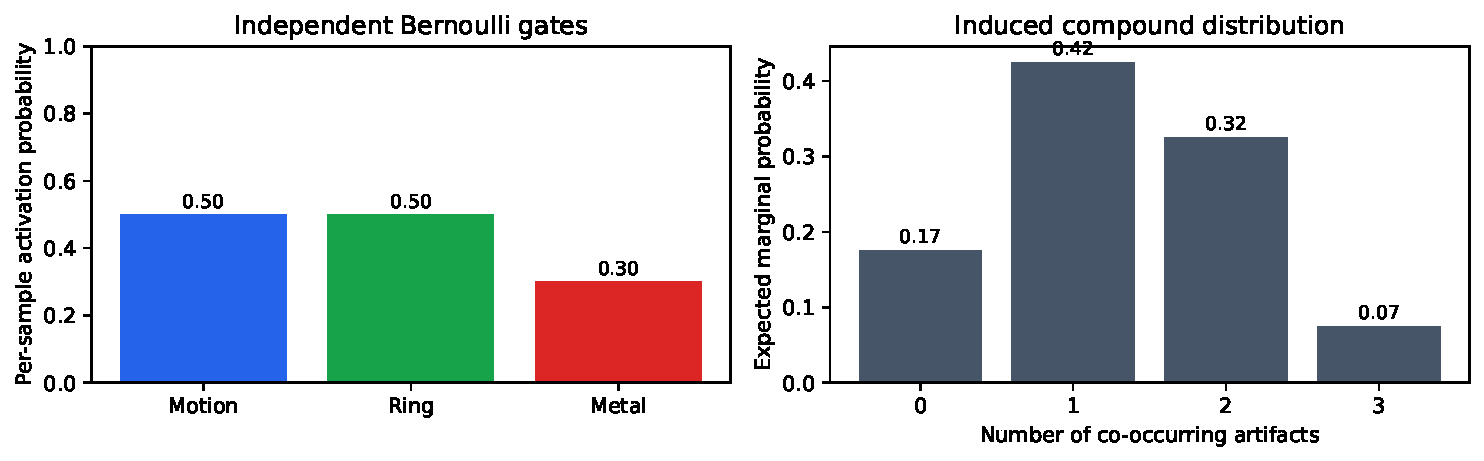
\includegraphics[width=\linewidth]{figures/fig_frequency.pdf}
    \caption[Per-artifact activation and induced compound distribution.]{%
        \textbf{Left:} per-sample Bernoulli activation probabilities for the three physical artifacts. \textbf{Right:}
        induced expected marginal distribution over the number of co-occurring artifacts under the independence assumption.}
    \label{fig:meth_frequency}
\end{figure}
The ordering in \eqref{eq:meth_compound} is chosen to preserve the intended structure of each corruption. Motion is applied first because it operates by interpolation along the detector axis; applying it after ring or metal injection would blur the sharp column-wise perturbations introduced by those artifacts. The final $[0,1]$ clipping step is required because the ring and metal operators can push a small number of bins slightly outside the physically valid range. Clipping removes these unphysical values while preserving consistency with the $\mu_{\max}$-normalized LoDoPaB representation.

\paragraph{Reproducibility of validation and test draws.}
For the training split, artifacts are sampled stochastically, so that each epoch presents a fresh realization of the corruption for every sample. This provides implicit data augmentation over the compound corruption distribution. For the validation and test splits, by contrast, the per-sample random number generator is seeded deterministically as $\mathrm{seed} + \mathrm{idx}$, ensuring that every epoch and every model is evaluated on exactly the same artifact realizations. As a result, comparisons between cascade variants in \Cref{chap:experiments} are not confounded by differences in the corruption draws.

\section{Protocol Validation}
\label{sec:meth_validation}

\Cref{fig:meth_artifact_examples} shows example sinograms and \gls{fbp} reconstructions for a single \mbox{LoDoPaB}
slice under each artifact in isolation and under the compound setting. The qualitative signatures match the physical
expectation: motion produces ghosting and edge-blurring on sharp tissue interfaces; ring artifacts appear as faint
concentric circles inside the patient cross-section; metal produces localized streaks radiating from the implant shadow
location; and the compound case overlays all three in a clinically plausible pattern.
\Cref{fig:meth_severity} complements this with a severity sweep at three operating points per artifact, demonstrating
that the parameter ranges in Tables~\ref{tab:meth_motion_params}--\ref{tab:meth_metal_params} span the
visible-but-not-destructive regime.

\begin{figure}[p]
    \vspace*{0pt}
    \centering
    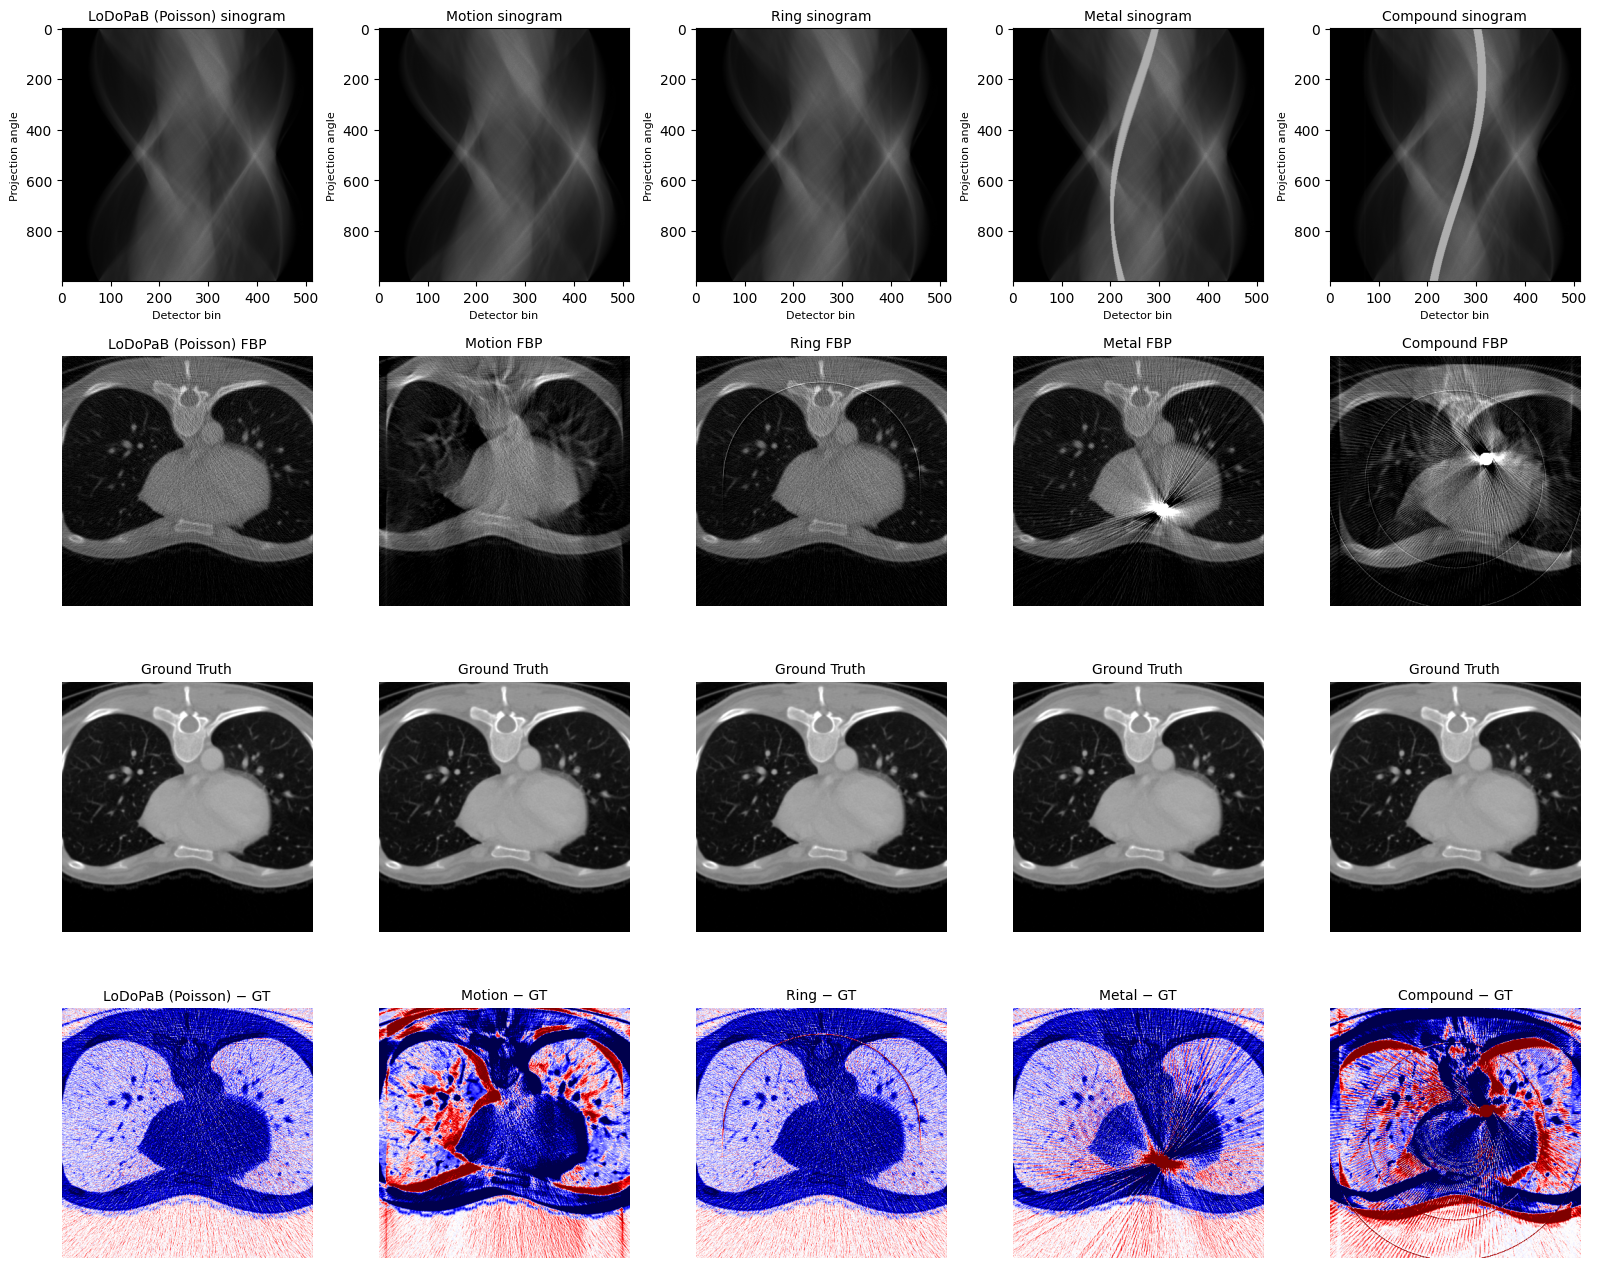
\includegraphics[width=\linewidth]{figures/fig_artifact_examples.png}
    \caption[Qualitative comparison of single and compound artifacts.]{%
        Sinogram (top), \gls{fbp} reconstruction (middle), and signed reconstruction error relative to the ground truth (bottom) for a representative \mbox{LoDoPaB} test slice under each artifact applied in isolation and under the full compound corruption setting. Images are displayed using the \mbox{LoDoPaB} window $[0, 0.45]$~\cite{Leuschner2021}; the error maps use a diverging window of $[-0.1, 0.1]$.}
    \label{fig:meth_artifact_examples}
\end{figure}

\begin{figure}[!htb]
    \centering
    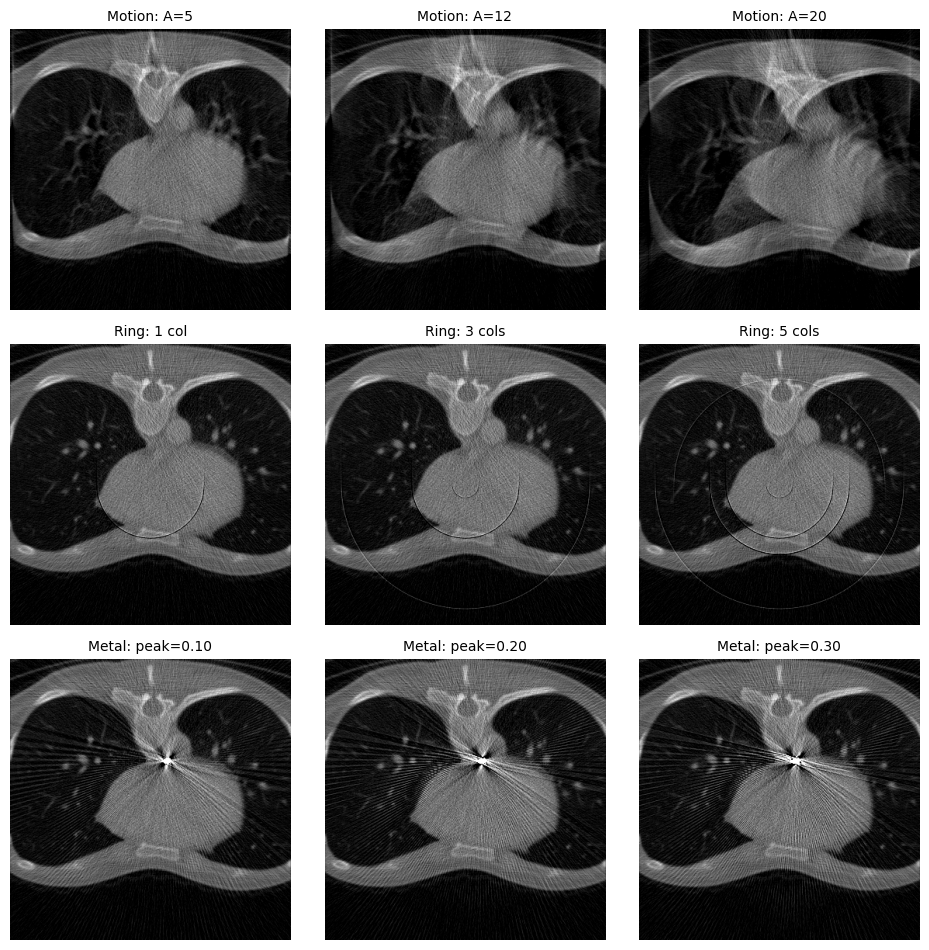
\includegraphics[width=0.95\linewidth]{figures/fig_severity_sweep.png}
    \caption[Severity sweep for each artifact type.]{%
        \gls{fbp} reconstructions shown at three severity levels for each artifact type. The parameter ranges used during training are chosen to span a regime in which the degradations are clearly perceptible while the underlying anatomical structure remains interpretable.}
    \label{fig:meth_severity}
\end{figure}
% \FloatBarrier
%%%%%%%% Cascaded Encoder-- Decoder Architectures
\section{Cascaded Encoder--Decoder Architectures}
\label{sec:meth_arch}
\label{chap:architectures}

This section describes the restoration models evaluated in this thesis. All first stages and all naive-cascade second stages use a plain U-Net backbone~\cite{Ronneberger2015}. Residual-cascade second stages use a ResUNet variant in which every convolutional block is equipped with an intra-block residual shortcut; this architectural change is described in \Cref{subsec:meth_cascade_variants}. Beyond the backbone choice, models differ along three axes: (a)~the number of stages, (b)~the input channels provided to the second stage, and (c)~the way gradients propagate between stages during training.

\subsection{Single-stage U-Net backbone}
\label{subsec:meth_unet}
The backbone is a standard U-Net~\cite{Ronneberger2015} with three downsampling levels and a symmetric upsampling path. Each encoder block consists of two $3{\times}3$ convolutions with GroupNorm and ReLU activations; downsampling is performed by $2{\times}2$ max-pooling. The decoder mirrors the encoder with bilinear upsampling, concatenation-based skip connections at each resolution level, and a final $1{\times}1$ convolution that produces the single-channel output through a sigmoid activation, constraining the prediction to $[0,1]$.

Two capacity configurations are evaluated throughout this work. The \emph{small} variant uses encoder channel widths $[32, 64, 128, 256]$ and has \num{1798113} parameters; the \emph{large} variant uses widths $[64, 128, 256, 512]$ and has \num{7184321} parameters. The resulting single-stage model,
\begin{equation}
    \hat{\mathbf{x}} \;=\; f_{\boldsymbol{\theta}}(\mathbf{y}),
    \label{eq:meth_unet_single}
\end{equation}
is trained end-to-end from scratch and serves both as the standalone baseline and as the first stage of all two-stage cascades introduced in the following.

\subsection{Two-stage cascade: Stage-2 input design}
\label{subsec:meth_cascade_input}

A second stage is introduced to allow further image-domain refinement. In all cascade variants, Stage~1 takes the single-channel Ram--Lak \gls{fbp} reconstruction $\mathbf{y}$ as its input and produces a restored estimate $\hat{\mathbf{x}}_1$. By default, Stage~2 receives only this estimate as a single-channel input:
\begin{equation}
    \mathbf{u}_2 \;=\; \hat{\mathbf{x}}_1.
    \label{eq:meth_default_input}
\end{equation}
This increases processing depth but does not introduce any additional measurement information beyond what is already encoded in $\hat{\mathbf{x}}_1$.

\paragraph{Dual-filter variant.}
One configuration studied in this work augments the Stage~2 input with two additional \gls{fbp} reconstructions computed from the same corrupted sinogram $\tilde{\mathbf{s}}$ using alternative reconstruction filters:
\begin{equation}
    \mathbf{u}_2^{(\mathrm{dual})}
    \;=\; \bigl[\,\hat{\mathbf{x}}_1\;\Vert\;\mathbf{y}^{(\mathrm{Hann})}\;\Vert\;\mathbf{y}^{(\mathrm{SL})}\,\bigr],
    \qquad
    \mathbf{y}^{(h)} \;=\; \mathcal{R}^{-1}_{h}\!\bigl(\tilde{\mathbf{s}}\bigr),
    \label{eq:meth_alt_input}
\end{equation}
where $\mathbf{y}^{(\mathrm{Hann})}$ and $\mathbf{y}^{(\mathrm{SL})}$ denote \gls{fbp} reconstructions produced with the Hann and Shepp--Logan filters, respectively, and $\Vert$ denotes channel-wise concatenation, giving Stage~2 a three-channel input. Different reconstruction filters realize different trade-offs between noise suppression and spatial resolution~\cite{KakSlaney1988}: Ram--Lak preserves sharp detail but amplifies noise, whereas Hann and Shepp--Logan produce smoother images at the cost of reduced high-frequency structure. Providing all three to Stage~2 supplies complementary image-domain information without introducing a learned sinogram-domain component. The resulting cascade is therefore not a dual-domain method~\cite{Wang2020, Zhang2022}, but a multi-input image-domain cascade.

In all variants that do not use the dual-filter extension, Stage~2 receives only $\hat{\mathbf{x}}_1$ (one channel). The dual-filter variant is evaluated only in combination with the residual cascade and is explicitly labelled throughout \Cref{chap:experiments}.
%%─────────────────────────────────────────────────────────
%% Three coupling variants
%%─────────────────────────────────────────────────────────
\subsection{Three coupling variants}
\label{subsec:meth_cascade_variants}

Given the two-stage backbone, three variants are defined by how the parameters
$\{\boldsymbol{\theta}_1, \boldsymbol{\theta}_2\}$ are optimized.

\paragraph{Independent-stage cascade.}
Both stages are trained simultaneously under the cascade loss
$\mathcal{L}^{\mathrm{cascade}}$ of \Cref{eq:meth_loss_cascade_weighted}, but with a
stop-gradient operator applied to $\hat{\mathbf{x}}_{1}$ before it enters Stage~2:
\begin{equation}
    \hat{\mathbf{x}}_{2}
    \;=\; f_{\boldsymbol{\theta}_{2}}\!\bigl(\mathrm{sg}(\mathbf{u}_2)\bigr),
    \label{eq:meth_ind_input}
\end{equation}
where $\mathrm{sg}(\cdot)$ denotes the stop-gradient operator and $\mathbf{u}_2$ is the Stage-2
input defined in \Cref{eq:meth_default_input,eq:meth_alt_input}. Stage~1 is supervised directly
by $\mathcal{L}^{(1)}$; the gradient of $\mathcal{L}^{(2)}$ is blocked at the stage boundary
and does not reach $\boldsymbol{\theta}_1$. Stage~2 is updated only by $\mathcal{L}^{(2)}$.
The two parameter sets are therefore optimized concurrently but with fully decoupled gradient
signals.

\paragraph{End-to-end cascade.}
Both stages are trained jointly under the weighted loss
$\mathcal{L}^{\mathrm{cascade}}$ of \Cref{eq:meth_loss_cascade_weighted},
applied to
\begin{equation}
    \hat{\mathbf{x}}_{2}
    \;=\; f_{\boldsymbol{\theta}_{2}}\!\bigl(\mathbf{u}_2\bigr).
    \label{eq:meth_e2e_input}
\end{equation}
Gradients flow through both stages, allowing earlier-stage features to specialize in service of the
final output. The per-stage weights $(w_{1}, w_{2}) = (0.5,\,0.5)$ in
\Cref{eq:meth_loss_cascade_weighted} mitigate the vanishing-gradient risk of the longer optimization
chain~\cite{He2016}.

\paragraph{Residual cascade.}
Stage~2 is reformulated to predict an additive correction to Stage~1 rather than the clean image directly:
\begin{equation}
    \hat{\mathbf{x}}_{2} \;=\; \hat{\mathbf{x}}_{1}
        \,+\, f_{\boldsymbol{\theta}_{2}}\!\bigl(\mathbf{u}_2\bigr),
    \label{eq:meth_residual}
\end{equation}
where $\mathbf{u}_2$ is either $\hat{\mathbf{x}}_1$ (single-channel default) or $\mathbf{u}_2^{(\mathrm{dual})}$ (\Cref{eq:meth_alt_input}) for the dual-filter variant. Stage~2 in the residual cascade uses a \emph{ResUNet} backbone --- identical in encoder--decoder structure to the U-Net of \Cref{subsec:meth_unet} but with every DoubleConv block replaced by a ResidualDoubleConv block that adds an intra-block shortcut connection and applies its final ReLU to the sum of the convolutional path and the shortcut. The output activation is \texttt{tanh} rather than sigmoid, allowing Stage~2 to predict both positive and negative corrections; the final image is obtained by clamping $\hat{\mathbf{x}}_2$ to $[0,1]$ after the addition in \Cref{eq:meth_residual}.

The residual cascade is trained with the independent-stage protocol ---
both stages trained simultaneously, with the stop-gradient operator applied to
$\hat{\mathbf{x}}_{1}$ so that gradients from $\mathcal{L}^{\mathrm{res}}$ do not reach
$\boldsymbol{\theta}_1$ --- under the three-term loss
$\mathcal{L}^{\mathrm{res}}$ of \Cref{eq:meth_loss_residual}. The residual $\ell^{1}$ term penalizes
the predicted correction directly, while the SSIM and gradient terms supervise the structural and
edge fidelity of the final image.

It should be noted that the residual cascade differs from the naive independent cascade along three dimensions simultaneously: (i)~the Stage~2 output representation changes from a direct image prediction to an additive correction; (ii)~the Stage~2 loss changes from the balanced SSIM\,+\,$\ell^{1}$ objective to the three-term residual loss $\mathcal{L}^{\mathrm{res}}$; and (iii)~the Stage~2 backbone changes from a plain U-Net to a ResUNet with intra-block residual shortcuts. Because no ablation isolates each factor independently, any performance difference observed in \Cref{chap:experiments} reflects the combined effect of all three changes and cannot be attributed to any single design choice alone.


%%─────────────────────────────────────────────────────────
%% Asymmetric-capacity probe
%%─────────────────────────────────────────────────────────
\subsection{Asymmetric-capacity probe}
\label{subsec:meth_asymmetric}

The three coupling variants of \Cref{subsec:meth_cascade_variants} hold stage capacity fixed:
both stages share the same channel widths. This leaves open a separate question about
\emph{capacity allocation}: if Stage~1 is given more parameters, does Stage~2 receive a cleaner
input and therefore converge to a better solution, or does the gain saturate regardless of how
capacity is distributed between stages?

To probe this we define two \emph{asymmetric} cascade configurations that re-allocate the total
parameter budget between the two stages:
\begin{itemize}
    \item \textbf{Large\,$\to$\,small.} Stage~1 uses the large U-Net (channel widths
        $[48,96,192,384]$, ${\approx}4.04$\,M parameters); Stage~2 uses the small ResUNet
        (channel widths $[16,32,64,128]$, ${\approx}0.47$\,M parameters). The hypothesis is
        that a stronger Stage~1 reduces the residual error handed to Stage~2, which Stage~2
        should then find easier to correct even with fewer parameters.
    \item \textbf{Small\,$\to$\,large.} Stage~1 uses the small U-Net (channel widths
        $[16,32,64,128]$, ${\approx}0.45$\,M parameters); Stage~2 uses the large ResUNet
        (channel widths $[48,96,192,384]$, ${\approx}4.24$\,M parameters). This tests the converse:
        whether greater Stage~2 capacity can compensate for a weaker Stage~1 input.
\end{itemize}
Both asymmetric configurations are trained with the independent-stage residual protocol
(\Cref{subsec:meth_cascade_variants}): both stages train simultaneously, with the stop-gradient
operator applied to $\hat{\mathbf{x}}_{1}$ so that Stage~2 is updated only by
$\mathcal{L}^{(2)}$ and Stage~1 only by $\mathcal{L}^{(1)}$. If the cascade gain is primarily
limited by \emph{available residual information} --- that is, by what Stage~1 failed to correct
--- then large\,$\to$\,small should outperform small\,$\to$\,large even though the latter has
more Stage~2 capacity. Conversely, if the gain is limited by Stage~2's representational ability,
the small\,$\to$\,large configuration should close the gap. The experimental outcomes are reported
in \Cref{sec:exp_quantitative}.

\Cref{tab:meth_model_configs} summarizes the backbone, feature widths, input channels, and parameter counts for all model configurations studied in this thesis.

\clearpage
\begin{table}[!ht]
    \centering
    \caption[Architecture and parameter counts for all studied model configurations.]{%
        Architecture and parameter counts for all model configurations. Stage~1 always uses the plain U-Net backbone with sigmoid output. Stage~2 in the naive cascade uses the same plain U-Net; Stage~2 in the residual cascade uses the ResUNet backbone with tanh output. The dual-filter extension adds the Hann and Shepp--Logan \gls{fbp} reconstructions as two extra input channels to Stage~2, increasing its input from 1 to 3 channels.}
    \label{tab:meth_model_configs}
    \setlength{\tabcolsep}{4pt}
    \small
    \begin{tabular}{@{}llllrr@{}}
        \toprule
        Configuration & Stage & Backbone & Features & in\_ch & Params \\
        \midrule
        \multicolumn{6}{l}{\textit{Single-stage baselines}} \\
        U-Net (small)  & Stage~1 & U-Net   & $[32,64,128,256]$  & 1 & \num{1798113} \\
        U-Net (large)  & Stage~1 & U-Net   & $[64,128,256,512]$ & 1 & \num{7184321} \\
        \midrule
        \multicolumn{6}{l}{\textit{Naive cascade — U-Net\,+\,U-Net (sigmoid)}} \\
        Small\,+\,small (detach / e2e)
                       & Stage~1 & U-Net   & $[32,64,128,256]$  & 1 & \num{1798113} \\
                       & Stage~2 & U-Net   & $[32,64,128,256]$  & 1 & \num{1798113} \\
        Large\,+\,large (detach)
                       & Stage~1 & U-Net   & $[48,96,192,384]$  & 1 & \num{4042705} \\
                       & Stage~2 & U-Net   & $[48,96,192,384]$  & 1 & \num{4042705} \\
        \midrule
        \multicolumn{6}{l}{\textit{Residual cascade — U-Net\,+\,ResUNet (tanh)}} \\
        Symmetric small
                       & Stage~1 & U-Net   & $[32,64,128,256]$  & 1 & \num{1798113} \\
                       & Stage~2 & ResUNet & $[32,64,128,256]$  & 1 & \num{1884865} \\
        Symmetric small (dual-filter)
                       & Stage~1 & U-Net   & $[32,64,128,256]$  & 1 & \num{1798113} \\
                       & Stage~2 & ResUNet & $[32,64,128,256]$  & 3 & \num{1885505} \\
        Asym.\ large$\to$small
                       & Stage~1 & U-Net   & $[48,96,192,384]$  & 1 & \num{4042705} \\
                       & Stage~2 & ResUNet & $[16,32,64,128]$   & 1 & \num{472417}  \\
        Asym.\ small$\to$large
                       & Stage~1 & U-Net   & $[16,32,64,128]$   & 1 & \num{450545}  \\
                       & Stage~2 & ResUNet & $[48,96,192,384]$  & 1 & \num{4237345} \\
        \bottomrule
    \end{tabular}
\end{table}

\Cref{fig:meth_cascade_variants} summarizes the data flow and all architectural variants
defined in \Crefrange{subsec:meth_unet}{subsec:meth_asymmetric}.

%% architecture figure
\begin{figure}[!htb]
\centering
%%─────────────────────────────────────────────────────────
%% (a)  Two-stage cascade: data flow
%%─────────────────────────────────────────────────────────
\begin{tikzpicture}[
    every node/.style={font=\footnotesize},
    blk/.style={rectangle, rounded corners=3pt, draw, very thick,
                minimum width=24mm, minimum height=12mm, align=center},
    io/.style={rectangle, rounded corners=2pt, draw,
               minimum width=14mm, minimum height=9mm,
               align=center, fill=gray!8},
    lossnd/.style={circle, draw, fill=yellow!20, minimum size=8mm},
    arr/.style={->, >=Stealth, thick},
    garr/.style={->, >=Stealth, thick, red!60!black, densely dashed},
    larr/.style={->, >=Stealth, gray, thin},
]
    \node[io] (y)    {$\mathbf{y}$\\[-2pt]\tiny Ram--Lak};
    \node[blk, fill=orange!10, right=10mm of y]  (stI)
        {Stage~1\\[-2pt]\tiny U-Net $f_{\theta_1}$};
    \node[io, right=10mm of stI] (x1)   {$\hat{\mathbf{x}}_1$};
    \node[circle, draw, fill=gray!12, minimum size=10mm,
          right=8mm of x1] (cat) {$\Vert$};
    \node[blk, fill=teal!10, right=8mm of cat]   (stII)
        {Stage~2\\[-2pt]\tiny U-Net $f_{\theta_2}$};
    \node[io, right=10mm of stII] (x2)   {$\hat{\mathbf{x}}_2$};
    \node[io, below=14mm of cat] (yalt)
        {$\mathbf{y}^{(\mathrm{Hann})},\mathbf{y}^{(\mathrm{SL})}$\\[-2pt]\tiny dual-filter only};

    %% Loss nodes
    \node[lossnd, below=8mm of x1, font=\tiny] (LI)  {$\mathcal{L}^{(1)}$};
    \node[lossnd, below=8mm of x2, font=\tiny] (LII) {$\mathcal{L}^{(2)}$};

    \draw[arr]  (y)    -- (stI);
    \draw[arr]  (stI)  -- (x1);
    \draw[arr]  (x1)   -- (cat);
    \draw[arr]  (yalt) -- (cat);
    \draw[arr]  (cat)  -- (stII);
    \draw[arr]  (stII) -- (x2);
    \draw[larr] (x1.south)  -- (LI);
    \draw[larr] (x2.south)  -- (LII);

    %% Backward gradient arc routed above the main row
    \coordinate (stIItop) at ([yshift=8mm]stII.north);
    \coordinate (stItop)  at ([yshift=8mm]stI.north);
    \draw[garr] (stII.north) -- (stIItop)
        -- node[above, font=\tiny, black, midway]
               {gradient path (variant-dependent; see (b)--(d))}
        (stItop) -- (stI.north);
\end{tikzpicture}

\bigskip
%%─────────────────────────────────────────────────────────
%% (b)(c)(d)  Coupling variants
%%─────────────────────────────────────────────────────────
\noindent
\begin{minipage}[t]{0.30\linewidth}
\centering
\begin{tikzpicture}[
    every node/.style={font=\footnotesize},
    sblk/.style={rectangle, rounded corners=2pt, draw, thick,
                 minimum width=16mm, minimum height=9mm, align=center},
    arr/.style={->, >=Stealth},
    larr/.style={->, >=Stealth, gray, thin},
]
    \node[sblk, fill=orange!10] (sta) {Stage~1};
    \node[sblk, fill=teal!10, right=14mm of sta] (stb) {Stage~2};
    \draw[arr] (sta) -- node[above, font=\tiny]{$\hat{\mathbf{x}}_1$} (stb);
    %% stop-gradient bar
    \path (sta.east) -- (stb.west) coordinate[midway] (sgm);
    \draw[very thick, red!70!black]
        ([yshift=4mm]sgm) -- ([yshift=-4mm]sgm);
    \node[font=\tiny, text=red!70!black, xshift=3mm] at (sgm) {sg};
    %% Loss nodes: each stage has its own
    \node[circle, draw, fill=yellow!20, minimum size=7mm,
          below=7mm of sta, font=\tiny] (La) {$\mathcal{L}^{(1)}$};
    \node[circle, draw, fill=yellow!20, minimum size=7mm,
          below=7mm of stb, font=\tiny] (Lb) {$\mathcal{L}^{(2)}$};
    \draw[larr] (sta.south) -- (La);
    \draw[larr] (stb.south) -- (Lb);
\end{tikzpicture}\\[4pt]
\small\textbf{(b)~Independent}\\[1pt]
{\tiny Both stages train simultaneously.\\ $\mathcal{L}^{(2)}$ gradient blocked (sg);\\ Stage~1 updated by $\mathcal{L}^{(1)}$ only.}
\end{minipage}%
\hfill
\begin{minipage}[t]{0.30\linewidth}
\centering
\begin{tikzpicture}[
    every node/.style={font=\footnotesize},
    sblk/.style={rectangle, rounded corners=2pt, draw, thick,
                 minimum width=16mm, minimum height=9mm, align=center},
    arr/.style={->, >=Stealth},
    garr/.style={->, >=Stealth, red!60!black, densely dashed},
    larr/.style={->, >=Stealth, gray, thin},
]
    \node[sblk, fill=orange!10] (sta) {Stage~1};
    \node[sblk, fill=teal!10, right=14mm of sta] (stb) {Stage~2};
    \draw[arr] (sta) -- node[above, font=\tiny]{$\hat{\mathbf{x}}_1$} (stb);
    %% Loss nodes
    \node[circle, draw, fill=yellow!20, minimum size=7mm,
          below=7mm of sta, font=\tiny] (La) {$\mathcal{L}^{(1)}$};
    \node[circle, draw, fill=yellow!20, minimum size=7mm,
          below=7mm of stb, font=\tiny] (Lb) {$\mathcal{L}^{(2)}$};
    \draw[larr] (sta.south) -- (La);
    \draw[larr] (stb.south) -- (Lb);
    %% Backward gradient arc (above): L^(2) gradient reaches Stage 1
    \coordinate (stbtop) at ([yshift=7mm]stb.north);
    \coordinate (statop) at ([yshift=7mm]sta.north);
    \draw[garr] (stb.north) -- (stbtop)
        -- node[above, font=\tiny, black, midway]{$\nabla$}
        (statop) -- (sta.north);
\end{tikzpicture}\\[4pt]
\small\textbf{(c)~End-to-end}\\[1pt]
{\tiny Both stages trained jointly.\\$\mathcal{L}^{(2)}$ gradient propagates\\back through Stage~1.}
\end{minipage}%
\hfill
\begin{minipage}[t]{0.36\linewidth}
\centering
\begin{tikzpicture}[
    every node/.style={font=\footnotesize},
    sblk/.style={rectangle, rounded corners=2pt, draw, thick,
                 minimum width=15mm, minimum height=9mm, align=center},
    arr/.style={->, >=Stealth},
    larr/.style={->, >=Stealth, gray, thin},
]
    \node[sblk, fill=orange!10] (sta) {Stage~1};
    \node[sblk, fill=teal!10, right=11mm of sta] (stb)
        {Stage~2\\\tiny pred.\ $\hat{\mathbf{r}}$};
    \node[circle, draw, fill=gray!12, minimum size=8mm,
          right=8mm of stb, font=\normalsize] (add) {$+$};
    \draw[arr] (sta) -- node[above, font=\tiny]{$\hat{\mathbf{x}}_1$} (stb);
    \draw[arr] (stb) -- node[above, font=\tiny]{$\hat{\mathbf{r}}$} (add);
    %% shortcut: x̂_1 enters + from above
    \draw[arr] (sta.north) -- ++(0,9mm) -| (add.north);
    %% stop-gradient bar
    \path (sta.east) -- (stb.west) coordinate[midway] (sgm2);
    \draw[very thick, red!70!black]
        ([yshift=4mm]sgm2) -- ([yshift=-4mm]sgm2);
    \node[font=\tiny, text=red!70!black, xshift=3mm] at (sgm2) {sg};
    %% Loss at final output
    \node[circle, draw, fill=yellow!20, minimum size=7mm,
          below=7mm of stb, font=\tiny] (La) {$\mathcal{L}^{(1)}$};
    \node[circle, draw, fill=yellow!20, minimum size=7mm,
          below=7mm of add, font=\tiny] (Lb) {$\mathcal{L}^{(2)}_\mathrm{res}$};
    \draw[larr] (sta.south) -- (La);
    \draw[larr] (add.south) -- (Lb);
\end{tikzpicture}\\[4pt]
\small\textbf{(d)~Residual}\\[1pt]
{\tiny Both stages train simultaneously;\\ Stage~2 predicts correction $\hat{\mathbf{r}}$;\\ $\hat{\mathbf{x}}_2 = \hat{\mathbf{x}}_1 + \hat{\mathbf{r}}$.}
\end{minipage}

\bigskip

%%─────────────────────────────────────────────────────────
%% (e)(f)  Asymmetric capacity
%%─────────────────────────────────────────────────────────
\noindent
\begin{minipage}[t]{0.46\linewidth}
\centering
\begin{tikzpicture}[
    every node/.style={font=\footnotesize},
    arr/.style={->, >=Stealth},
]
    \node[rectangle, rounded corners=2pt, draw, thick,
          fill=orange!20, minimum width=30mm, minimum height=11mm,
          align=center] (sta)
        {Stage~1\\[-2pt]\tiny Large U-Net ($4.04$\,M)};
    \node[rectangle, rounded corners=2pt, draw, thick,
          fill=teal!8, minimum width=20mm, minimum height=11mm,
          align=center, right=12mm of sta] (stb)
        {Stage~2\\[-2pt]\tiny Small ResUNet ($0.47$\,M)};
    \draw[arr] (sta) -- node[above, font=\tiny]{$\hat{\mathbf{x}}_1$} (stb);
\end{tikzpicture}\\[4pt]
\small\textbf{(e)~Large $\to$ Small}
\end{minipage}%
\hfill
\begin{minipage}[t]{0.46\linewidth}
\centering
\begin{tikzpicture}[
    every node/.style={font=\footnotesize},
    arr/.style={->, >=Stealth},
]
    \node[rectangle, rounded corners=2pt, draw, thick,
          fill=orange!8, minimum width=20mm, minimum height=11mm,
          align=center] (sta)
        {Stage~1\\[-2pt]\tiny Small U-Net ($0.45$\,M)};
    \node[rectangle, rounded corners=2pt, draw, thick,
          fill=teal!20, minimum width=30mm, minimum height=11mm,
          align=center, right=12mm of sta] (stb)
        {Stage~2\\[-2pt]\tiny Large ResUNet ($4.24$\,M)};
    \draw[arr] (sta) -- node[above, font=\tiny]{$\hat{\mathbf{x}}_1$} (stb);
\end{tikzpicture}\\[4pt]
\small\textbf{(f)~Small $\to$ Large}
\end{minipage}

\caption[Cascade architecture variants.]{%
    \textbf{(a)}~General two-stage cascade data flow. The corrupted FBP
    reconstruction $\mathbf{y}$ (Ram--Lak filter) feeds Stage~1; its output
    $\hat{\mathbf{x}}_1$ forms the Stage~2 input $\mathbf{u}_2$ (single channel by default;
    three channels $[\hat{\mathbf{x}}_1\,\Vert\,\mathbf{y}^{(\mathrm{Hann})}\,\Vert\,\mathbf{y}^{(\mathrm{SL})}]$
    in the dual-filter variant).
    Loss nodes $\mathcal{L}^{(1)}$ and $\mathcal{L}^{(2)}$ supervise
    each stage output. The dashed red arc marks the backward gradient path,
    which is variant-dependent.
    \textbf{(b)~Independent:} both stages train simultaneously; the
    stop-gradient barrier (sg) blocks the $\mathcal{L}^{(2)}$ gradient from
    reaching Stage~1, which is updated only by $\mathcal{L}^{(1)}$.
    \textbf{(c)~End-to-end:} both stages trained jointly; the
    $\mathcal{L}^{(2)}$ gradient $\nabla$ propagates back through Stage~2
    and continues to update Stage~1.
    \textbf{(d)~Residual:} same stop-gradient protocol as (b); Stage~2
    predicts an additive correction $\hat{\mathbf{r}}$, giving
    $\hat{\mathbf{x}}_2 = \hat{\mathbf{x}}_1 + \hat{\mathbf{r}}$;
    the arc above shows the $\hat{\mathbf{x}}_1$ shortcut.
    \textbf{(e)--(f)}~Asymmetric-capacity configurations; block width is
    proportional to parameter count.}
\label{fig:meth_cascade_variants}
\end{figure}

\FloatBarrier

%%─────────────────────────────────────────────────────────
%% section:Loss function
%%─────────────────────────────────────────────────────────
\section{Loss Functions}
\label{sec:meth_loss}

A pure pixel-wise $\ell^{1}$ loss, although widely used in CT restoration and denoising~\cite{Chen2017, Zhang2017}, was found in preliminary experiments to over-smooth high-frequency anatomical detail under the compound-corruption regime considered here. Conversely, pure \gls{ssim} supervision preserved structure well but allowed slight residual intensity drift in smooth regions. We therefore adopt a mixed loss that combines \gls{ssim} with $\ell^{1}$ and, for the residual cascade, an additional finite-difference gradient term to sharpen edges near metal streaks. To keep notation compact, let $\mathcal{L}_{1}$, $\mathcal{L}_{\mathrm{SSIM}}$, and $\mathcal{L}_{\nabla}$ denote, respectively, the pixel-wise \gls{mae}, the structural-similarity loss \(1-\mathrm{SSIM}\)~\cite{Wang2004}, and a finite-difference image-gradient $\ell^{1}$ loss,
\begin{align}
    \mathcal{L}_{1}(\hat{\mathbf{x}}, \mathbf{x}) &\;=\; \frac{1}{HW}\sum_{j}\bigl|\hat{x}_{j} - x_{j}\bigr|,
    \label{eq:meth_l1_loss}\\
    \mathcal{L}_{\mathrm{SSIM}}(\hat{\mathbf{x}}, \mathbf{x}) &\;=\; 1 - \mathrm{SSIM}(\hat{\mathbf{x}}, \mathbf{x}),
    \label{eq:meth_ssim_loss}\\
    \mathcal{L}_{\nabla}(\hat{\mathbf{x}}, \mathbf{x})
        &\;=\; \frac{1}{HW}\sum_{j}\Bigl(
        |\nabla_{x}\hat{x}_{j}-\nabla_{x}x_{j}|
        + |\nabla_{y}\hat{x}_{j}-\nabla_{y}x_{j}|
        \Bigr).
    \label{eq:meth_grad_loss}
\end{align}
These primitive losses are combined into task-specific objectives that are reused across the cascade variants.

\paragraph{Stage~1 --- balanced SSIM + L1.}
Stage~1 is supervised using an equal-weight combination of \gls{ssim} and pixel-wise \gls{mae},
\begin{equation}
    \mathcal{L}^{(1)}\!\bigl(\hat{\mathbf{x}}_{1}, \mathbf{x}\bigr)
    \;=\; 0.5\,\mathcal{L}_{\mathrm{SSIM}}\!\bigl(\hat{\mathbf{x}}_{1}, \mathbf{x}\bigr)
    \;+\; 0.5\,\mathcal{L}_{1}\!\bigl(\hat{\mathbf{x}}_{1}, \mathbf{x}\bigr).
    \label{eq:meth_loss_stage1}
\end{equation}
The \gls{ssim} term promotes local structural agreement with the reference image, while the $\ell^{1}$ term anchors absolute intensity values and reduces low-frequency drift in smooth regions.

\paragraph{Stage~2 in the naive cascade --- same SSIM + L1.}
In the naive cascade variants, Stage~2 predicts the restored image directly and is trained with the same balanced objective,
\begin{equation}
    \mathcal{L}^{(2)}_{\mathrm{naive}}\!\bigl(\hat{\mathbf{x}}_{2}, \mathbf{x}\bigr)
    \;=\; 0.5\,\mathcal{L}_{\mathrm{SSIM}}\!\bigl(\hat{\mathbf{x}}_{2}, \mathbf{x}\bigr)
    \;+\; 0.5\,\mathcal{L}_{1}\!\bigl(\hat{\mathbf{x}}_{2}, \mathbf{x}\bigr).
    \label{eq:meth_loss_naive_stage2}
\end{equation}
Using the same loss in both stages keeps the comparison between the single-stage baseline and the naive two-stage cascades clean: any performance difference is attributable to architectural design or coupling strategy rather than to a change in the objective.

\paragraph{Stage~2 in the residual cascade --- residual L1 + SSIM + gradient.}
In the residual cascade, Stage~2 predicts an additive correction
\[
    \hat{\mathbf{r}}_{2}
    = f_{\boldsymbol{\theta}_{2}}\!\bigl(\mathbf{u}_2\bigr),
\]
with final output \(\hat{\mathbf{x}}_{2}=\hat{\mathbf{x}}_{1}+\hat{\mathbf{r}}_{2}\). It is trained using a three-term loss that penalises the residual prediction itself, the structural quality of the final image, and the fidelity of edge information,
\begin{equation}
    \mathcal{L}^{(2)}_{\mathrm{res}}
    \;=\; 0.4\,\mathcal{L}_{1}\!\bigl(\hat{\mathbf{r}}_{2}, \mathbf{r}\bigr)
    \;+\; 0.3\,\mathcal{L}_{\mathrm{SSIM}}\!\bigl(\hat{\mathbf{x}}_{2}, \mathbf{x}\bigr)
    \;+\; 0.3\,\mathcal{L}_{\nabla}\!\bigl(\hat{\mathbf{x}}_{2}, \mathbf{x}\bigr),
    \label{eq:meth_loss_residual}
\end{equation}
where \(\mathbf{r}=\mathbf{x}-\hat{\mathbf{x}}_{1}\) denotes the target residual. The gradient term compensates for the soft-edge bias that pure SSIM/\(\ell^{1}\) supervision would otherwise leave near sharp metal-streak boundaries.

\paragraph{Per-stage weighting in cascades.}
Whenever a cascade is trained under a single joint objective, both stage outputs contribute with equal weight,
\begin{equation}
    \mathcal{L}^{\mathrm{cascade}}
    \;=\; 0.5\,\mathcal{L}^{(1)}\!\bigl(\hat{\mathbf{x}}_{1}, \mathbf{x}\bigr)
    \;+\; 0.5\,\mathcal{L}^{(2)}\!\bigl(\hat{\mathbf{x}}_{2}, \mathbf{x}\bigr),
    \label{eq:meth_loss_cascade_weighted}
\end{equation}
where \(\mathcal{L}^{(2)}\) is either \eqref{eq:meth_loss_naive_stage2} or \eqref{eq:meth_loss_residual}. Equal per-stage weights provide explicit supervision to the intermediate output and reduce the risk that Stage~1 receives only weak training signals in the end-to-end setting.

A summary of the losses used by each model variant is given in \Cref{tab:meth_losses}.

\begin{table}[!htb]
    \centering
    \caption[Loss function per cascade variant.]{%
        Loss function used to train each model variant. When a cascade is monitored or optimized jointly, both stages contribute with equal weight \(w_{1}=w_{2}=0.5\). SSIM denotes the structural-similarity loss \(1-\mathrm{SSIM}\)~\cite{Wang2004}, and $\mathcal{L}_{\nabla}$ denotes the finite-difference image-gradient $\ell^{1}$ loss.}
    \label{tab:meth_losses}
    \setlength{\tabcolsep}{4pt}
    \small
    \begin{tabular}{@{}l l@{}}
        \toprule
        Variant & Loss \\
        \midrule
        Stage~1 (single-stage U-Net) &
        $0.5\,\mathcal{L}_{\mathrm{SSIM}}(\hat{\mathbf{x}}_{1},\mathbf{x}) + 0.5\,\mathcal{L}_{1}(\hat{\mathbf{x}}_{1},\mathbf{x})$ \\
        Independent-stage naive cascade (Stage~2) &
        $0.5\,\mathcal{L}_{\mathrm{SSIM}}(\hat{\mathbf{x}}_{2},\mathbf{x}) + 0.5\,\mathcal{L}_{1}(\hat{\mathbf{x}}_{2},\mathbf{x})$ \\
        End-to-end naive cascade &
        $0.5\,\mathcal{L}^{(1)}(\hat{\mathbf{x}}_{1},\mathbf{x}) + 0.5\,\mathcal{L}^{(2)}_{\mathrm{naive}}(\hat{\mathbf{x}}_{2},\mathbf{x})$ \\
        Independent-stage residual cascade &
        $0.4\,\mathcal{L}_{1}(\hat{\mathbf{r}}_{2},\mathbf{r}) + 0.3\,\mathcal{L}_{\mathrm{SSIM}}(\hat{\mathbf{x}}_{2},\mathbf{x}) + 0.3\,\mathcal{L}_{\nabla}(\hat{\mathbf{x}}_{2},\mathbf{x})$ \\
        End-to-end residual cascade &
        $0.5\,\mathcal{L}^{(1)}(\hat{\mathbf{x}}_{1},\mathbf{x}) + 0.5\,\mathcal{L}^{(2)}_{\mathrm{res}}$ \\
        \bottomrule
    \end{tabular}
\end{table}
%%─────────────────────────────────────────────────────────
%% Training Procedure
%%─────────────────────────────────────────────────────────
\section{Training Procedure}
\label{sec:meth_training}

All models are trained on the \mbox{LoDoPaB-CT} \texttt{train} split (\num{35820} slices), with the sinogram-domain corruption pipeline of \Cref{sec:meth_compound} applied on the fly during data loading. Model selection is performed on the \texttt{validation} split (\num{3522} slices), and final quantitative results in \Cref{chap:experiments} are reported on the held-out \texttt{test} split (\num{3553} slices). For the validation and test sets, the corruption process is seeded deterministically on a per-sample basis, so that every model is evaluated on exactly the same artifact realizations. No external data are used at any stage: in particular, we do not use clean-CT pre-training, synthetic pretraining on auxiliary datasets, or out-of-domain medical images.

Optimization is carried out using AdamW with the default momentum parameters $(\beta_{1}, \beta_{2}) = (0.9,\,0.999)$. Unless stated otherwise, the learning rate is fixed at $3\times 10^{-4}$ for all proposed models. The only exception is the RED-CNN baseline, which is trained at $1\times 10^{-4}$ in order to match the original training protocol of Chen et al.~\cite{Chen2017}. The mini-batch size is $4$ slices, chosen to fit the U-Net-based models at resolution $362\times 362$ on a single \gls{gpu}. Each model is trained for up to $150$ epochs with early stopping: training is halted if the validation loss does not improve for $15$ consecutive epochs, and the checkpoint achieving the lowest validation loss is retained for final evaluation.

No augmentation beyond stochastic corruption sampling is applied. In particular, random geometric transforms such as flips or rotations are omitted in order to preserve a fixed image orientation throughout training and evaluation. For visual inspection only, images are displayed using the local viewing convention \texttt{np.flipud(x.T)}, but this is a display transform rather than part of the learning pipeline. The effective augmentation therefore comes entirely from the per-epoch resampling of corruption parameters on the training split, which exposes the network to fresh artifact realizations throughout optimization.

\section{Implementation and Known Simplifications}
\label{sec:meth_implementation}

\paragraph{Implementation.}
The corruption pipeline is implemented in \texttt{utils/lodopab\_dataset.py} and executed on the CPU inside the \texttt{Dataset.\_\_getitem\_\_} method. This design places the additional corruption cost in the \texttt{DataLoader} worker processes rather than in the GPU training loop, so artifact synthesis does not block model execution. The metal artifact component relies on a precomputed library generated once by \texttt{scripts/build\_metal\_library.py} on GPU and stored as a memory-mapped \texttt{.npz} file for efficient reuse at training time. In practice, the combined runtime for motion, ring, and metal corruption is only a few milliseconds per sample, and with eight data-loading workers the total artifact-injection overhead is approximately \SI{20}{\second} per epoch over the \num{35820} training slices. All experiments are implemented in PyTorch and run on a single \gls{gpu}.

\paragraph{Known simplifications.}
The corruption model is intentionally lightweight so that it can be applied online during training at negligible computational cost. To make the resulting scope explicit, we summarize the main modeling simplifications in the following.

\begin{enumerate}
    \item \textbf{Monoenergetic metal model.}
    The additive formulation in \eqref{eq:meth_metal_additive} assumes a monoenergetic acquisition model and therefore does not reproduce the full spectral beam-hardening behavior of polyenergetic CT. As a practical approximation, the missing amplification is absorbed empirically into the sampled metal-strength range $\alpha \in [0.10, 0.30]$, following common simplified practice in \gls{mar} simulation. The photon-starvation clipping term in \eqref{eq:meth_metal_starvation} captures the dominant count-rate nonlinearity, but not the full spectral signature associated with beam hardening. A fully polyenergetic forward simulation would require regenerating the measurement process rather than perturbing the fixed LoDoPaB sinograms, and is therefore left for future work.

    \item \textbf{One-dimensional motion projection.}
    The motion model applies the displacement in \eqref{eq:meth_motion_shift} only along the detector coordinate, effectively reducing in-plane motion to a single projected shift in the sinogram domain. This avoids a more expensive re-projection step while still representing the dominant radial component of respiratory motion that is most relevant for thoracic CT slices. The model therefore captures structured view-dependent inconsistency, but not the full angular coupling of independent two-dimensional translation.

    \item \textbf{Integer-bin metal translation.}
    The library-based metal contribution is shifted using integer detector-bin rolls rather than sub-bin interpolation. This introduces a small discretizations error, but in practice its effect is minor relative to the stochastic variation in sampled metal position and intensity, and is further attenuated by the subsequent photon-starvation clipping stage.
\end{enumerate}

These simplifications do not affect the central comparison in \Cref{chap:experiments}, because all model variants are trained and evaluated under the same seeded corruption distribution. The purpose of the protocol is not to reproduce scanner physics exhaustively, but to provide a controlled and repeatable stress test for comparing restoration architectures under consistent mixed-artifact conditions. More realistic polyenergetic simulation and higher-fidelity motion modeling are discussed as natural extensions in \Cref{chap:conclusion}.
        % Chapter 3: Methodology (corruption + cascade architectures)
\cleardoublepage
\chapter{Experiments and Results}
\label{chap:experiments}

This chapter evaluates cascaded image-domain encoder--decoder architectures on a corruption distribution that combines low-dose Poisson noise with the three sinogram-domain physical artifacts introduced in \Cref{sec:meth_compound}. To our knowledge, this joint setting has received limited attention in the literature: low-dose CT benchmarks typically isolate noise, whereas artifact-correction studies usually assume nominal photon flux. The protocol of \Cref{sec:meth_overview} is designed to bridge that gap and provides the experimental setting in which the second contribution of this work---the comparison of independent-stage, end-to-end, and residual cascade formulations---is assessed against matched single-network baselines.

The central finding of the chapter is that a single well-designed encoder--decoder already operates close to the practical image-domain ceiling on this protocol. Adding a second image-domain stage yields only limited benefit unless it is given access to new information. Among the cascade variants, the residual formulation produces a small but consistent improvement, while the gradient analysis later in the chapter helps explain why the end-to-end formulation does not.

\Cref{sec:exp_setup} defines the data, baselines, and evaluation metrics.
\Cref{sec:exp_baselines_table} reports the baseline reference results.
\Cref{sec:exp_cascade} presents the matched-capacity cascade comparison.
\Cref{sec:exp_asymmetric} examines the asymmetric-capacity setting.
\Cref{sec:exp_qualitative} shows representative qualitative examples.
\Cref{sec:exp_gradient} Analyzes per-stage gradient flow.
\Cref{sec:exp_discussion} discusses the implications and limitations of the findings.
%%─────────────────────────────────────────────────────────
%% Experimental setup
%%─────────────────────────────────────────────────────────
\section{Experimental Setup}
\label{sec:exp_setup}

\subsection{Dataset and corruption protocol}
\label{subsec:exp_dataset}

All models are trained and evaluated on the LoDoPaB-CT benchmark~\cite{Leuschner2021}, using the official train\,/\,validation\,/\,test split (\num{35820}\,/\,\num{3522}\,/\,\num{3553} slices). The corruption protocol described in \Cref{sec:meth_compound} is applied independently to each sample during batch construction. Low-dose Poisson noise is inherited from the LoDoPaB simulator (\(N_0=\num{4096}\) photons per pixel), while the three physical artifacts---motion, ring, and metal---are independently activated by per-sample Bernoulli draws with probabilities \((p_\mathrm{mot}, p_\mathrm{ring}, p_\mathrm{met}) = (0.5, 0.5, 0.3)\).

For the validation and test splits, the per-sample random number generator is seeded as \(\mathrm{seed}+\mathrm{idx}\), so that every method in this chapter is evaluated on an identical set of artifact realizations. All images are displayed using the LoDoPaB intensity window \([0, 0.45]\) on the \(\mu_{\max}\)-normalized scale~\cite{Leuschner2021}.
%%─────────────────────────────────────────────────────────
%% Baselines
%%─────────────────────────────────────────────────────────
\subsection{Baselines}
\label{subsec:exp_baselines}

Three classes of baseline are included in the comparison. The corrupted FBP reconstruction $\mathbf{y} = \mathcal{R}^{-1}\tilde{\mathbf{s}}$ provides the unrecovered input and therefore sets the minimum performance level that any restoration method must improve upon. \gls{bm3d}~\cite{Dabov2007} is applied directly to $\mathbf{y}$ as a classical non-learned reference; its noise parameter is selected by a five-point grid search on the validation set over $\sigma \in \{0.05, 0.075, 0.1, 0.15, 0.2\}$, yielding a best value of $\sigma = 0.10$.

\gls{redcnn}~\cite{Chen2017} is included as a learned single-network reference with \num{1842049} trainable parameters and is trained on the same corrupted/clean pairs as the cascade variants. Finally, a single-stage U-Net identical in architecture to the first stage of each cascade model is trained at two capacities: \emph{U-Net (small)} with \num{1798113} parameters (channel widths $[32, 64, 128, 256]$) and \emph{U-Net (large)} with \num{7184321} parameters (channel widths $[64, 128, 256, 512]$). These two U-Net configurations serve as matched-capacity references for the small and large cascade variants, respectively.
%%─────────────────────────────────────────────────────────
%% Cascade variants
%%─────────────────────────────────────────────────────────
\subsection{Cascade variants}
\label{subsec:exp_variants}

The three coupling formulations introduced in \Cref{sec:meth_arch} are evaluated.

\begin{description}
    \item[Independent-stage (naive).] Both stages are trained simultaneously under the cascade objective, but a stop-gradient operator is applied to $\hat{\mathbf{x}}_1$ at the stage boundary. As a result, Stage~1 is updated only by $\mathcal{L}^{(1)}$, while Stage~2 is updated only by $\mathcal{L}^{(2)}$.

    \item[End-to-end.] Both stages are trained jointly under the weighted loss $0.5\,\mathcal{L}^{(1)} + 0.5\,\mathcal{L}^{(2)}$, and gradients are allowed to propagate through the full cascade.

    \item[Residual.] Stage~2 predicts an additive correction $\hat{\mathbf{r}}_2$ to the Stage~1 output, as defined in \Cref{eq:meth_residual}, and is supervised using the residual loss $\mathcal{L}^{(2)}_{\mathrm{res}}$ from \Cref{eq:meth_loss_residual}. Unless stated otherwise, the reported residual models use the independent-stage training protocol.
\end{description}

Two additional configurations are included to test whether cascade performance is limited primarily by parameter allocation or by the information available to the second stage.

\begin{description}
    \item[Asymmetric capacity.] A small Stage~1 followed by a large Stage~2, and the converse arrangement, are evaluated as defined in \Cref{subsec:meth_asymmetric}. This tests whether redistributing model capacity across the two stages changes the marginal value of the cascade.

    \item[Dual-filter input to Stage~2.] The alternative-filter scheme of \Cref{eq:meth_alt_input} is used, in which Stage~2 receives $\hat{\mathbf{x}}_1$ concatenated with Hann- and Shepp--Logan-filtered FBP reconstructions of the same corrupted sinogram. This provides Stage~2 with additional image-domain information not present in the Ram--Lak input to Stage~1.
\end{description}
%%─────────────────────────────────────────────────────────
%% Evaluation metrics
%%─────────────────────────────────────────────────────────
\subsection{Evaluation metrics}
\label{subsec:exp_metrics}

Evaluation is reported in terms of \gls{psnr}, \gls{ssim}, and root-mean-square error (RMSE),
\begin{equation}
    \mathrm{RMSE}(\hat{\mathbf{x}}, \mathbf{x})
    = \sqrt{\tfrac{1}{HW}\sum_j (\hat{x}_j - x_j)^2}.
    \label{eq:exp_rmse}
\end{equation}
All metrics are computed per slice on the $\mu_{\max}$-normalized image and then averaged over the \num{3553} test slices. Before metric computation, model outputs are clamped to $[0,1]$. For PSNR, the dynamic range is set to $\mathrm{MAX}=1.0$, corresponding to the full $\mu_{\max}$-normalized intensity range of the images. The display window $[0,\,0.45]$ used for visualization~\cite{Leuschner2021, Kiss2024} is a windowing convention only and is not used as the PSNR denominator.

All cascade variants are trained for up to $150$ epochs with early stopping (patience $15$) and AdamW at a learning rate of $3\times 10^{-4}$ using identical seeded corruption draws. Joint losses use equal per-stage weights, $w_1 = w_2 = 0.5$. For the independent-stage variants, the stop-gradient operator at $\hat{\mathbf{x}}_1$ ensures that $\mathcal{L}^{(1)}$ and $\mathcal{L}^{(2)}$ update only the parameters of their respective stages throughout training.
%%─────────────────────────────────────────────────────────
%% Baseline References
%%─────────────────────────────────────────────────────────
\section{Baseline References}
\label{sec:exp_baselines_table}

\Cref{tab:exp_baselines} reports the five baseline reference methods.
Three observations motivate the cascade study that follows. First, the corrupted FBP input is substantially worse than the standard LoDoPaB noise-only setting reported in \cite{Leuschner2021}, confirming that the added physical artifacts materially increase the reconstruction difficulty beyond low-dose Poisson noise alone. Second, BM3D yields only a modest PSNR improvement over the corrupted input, although the gain in SSIM is more pronounced. This is consistent with its role as a classical denoiser that suppresses part of the stochastic noise but leaves structured artifacts largely unresolved.

\begin{table}[!htb]
    \centering
    \caption[Baseline references on LoDoPaB-CT under compound corruption.]{%
        Restoration quality on the LoDoPaB-CT test split
        (\num{3553} slices) under the full compound-corruption
        distribution. PSNR is computed on the $\mu_{\max}$-normalized image with
        $\mathrm{MAX}=1.0$ (full normalized range); model outputs are clamped to $[0,1]$
        before evaluation. The display window $[0,\,0.45]$~\cite{Leuschner2021} is used
        for visualization only and does not affect metric computation.}
    \label{tab:exp_baselines}
    \setlength{\tabcolsep}{6pt}
    \small
    \begin{tabular}{@{}l r r r r@{}}
        \toprule
        Method                              & Params    & PSNR (dB) & SSIM     & RMSE    \\
        \midrule
        Corrupted FBP (input)               & ---       & $21.49$   & $0.4488$ & $0.0869$ \\
        BM3D on FBP~\cite{Dabov2007}        & ---       & $22.14$   & $0.6814$ & $0.0806$ \\
        RED-CNN~\cite{Chen2017}             & $1.84$\,M & $27.03$   & $0.7107$ & $0.0500$ \\
        U-Net (small)                       & $1.80$\,M & $35.39$   & $0.8680$ & $0.0193$ \\
        U-Net (large)                       & $7.18$\,M & $\mathbf{36.11}$ & $\mathbf{0.8772}$ & $\mathbf{0.0178}$ \\
        \bottomrule
    \end{tabular}
\end{table}

Third, RED-CNN improves clearly over BM3D but remains well below the U-Net references, trailing even the smaller U-Net by more than \SI{8}{\decibel} in PSNR. Two architectural factors explain the gap. RED-CNN was originally designed for single-type Poisson noise at a fixed dose~\cite{Chen2017}: its encoder--decoder comprises only five convolutional layers per path without multi-resolution pooling, which limits the receptive field available for suppressing the spatially extended streaks and rings introduced by the compound-corruption protocol. The U-Net's skip connections and three-level pooling hierarchy provide a substantially larger effective receptive field, enabling it to integrate spatial context over the full extent of metal streaks and motion-induced ghosts. Inspection of loss curves (not shown) confirms that RED-CNN converged within the first 30 epochs under the present training protocol, ruling out insufficient training as an explanation for the gap. The two U-Net baselines therefore form the most relevant single-stage references for the cascade comparisons reported below.

\paragraph{Per-slice metric variability.}
All mean metrics reported in this chapter are computed over all \num{3553} test slices, which span a wide range of corruption severities. Per-slice standard deviations, evaluated for the two strongest models (U-Net large and the residual dual-filter cascade), are $\sigma_{\mathrm{PSNR}} \approx \SI{4.4}{\decibel}$ and $\sigma_{\mathrm{SSIM}} \approx 0.12$. These large spreads reflect the inherent variability of the compound corruption protocol: noise-only slices reach up to $\SI{39.6}{\decibel}$ on average, while triple-artifact slices fall to approximately $\SI{33.9}{\decibel}$ (see \Cref{tab:exp_per_artifact}). The mean differences between cascade variants (typically $0.15$--$0.72$\,dB) are therefore small relative to the within-test-set spread. They are, however, consistent across the full \num{3553}-slice evaluation and align with the qualitative and gradient evidence presented in the following sections.
%%─────────────────────────────────────────────────────────
%% Cascade Comparison at Matched Capacity
%%─────────────────────────────────────────────────────────
\section{Cascade Comparison at Matched Capacity}
\label{sec:exp_cascade}
\label{sec:exp_quantitative}

\Cref{tab:exp_cascade} compares the three cascade formulations against the small single-stage U-Net at matched per-stage capacity. All cascade rows use a small$+$small configuration, so any gain over the small single-stage reference reflects the effect of staging rather than a larger first-stage backbone. The large single-stage U-Net is included as an upper reference. For clarity, the table reports only the final cascade output (Stage~2); Stage~1 results are shown separately in \Cref{fig:exp_stage_improvement}.

The ordering in $\Delta$PSNR is unambiguous. Adding a second image-domain stage under the naive independent protocol improves the small U-Net by only $+0.15$\,dB, indicating that a simple serial decomposition yields little benefit on its own. End-to-end coupling increases this gain to $+0.46$\,dB, and the residual formulation increases it further to $+0.54$\,dB. The best matched-capacity result is obtained by the residual cascade with dual-filter input, which reaches $+0.72$\,dB over the small single-stage U-Net and matches the PSNR of the large single-stage reference.

\begin{table}[!htb]
    \centering
    \caption[Cascade comparison at matched per-stage capacity.]{%
        Cascade output (Stage~2) on the LoDoPaB-CT test split. All cascade
        rows use small$+$small per-stage capacity and are compared against
        the small single-stage U-Net. The large single-stage U-Net is
        included as an upper reference. The best result among the
        matched-capacity rows is shown in \textbf{bold}. $\Delta$PSNR denotes
        the gain over the small single-stage U-Net.}
    \label{tab:exp_cascade}
    \setlength{\tabcolsep}{6pt}
    \small
    \begin{tabular}{@{}l r r r r r@{}}
        \toprule
        Method                                     & Params      & PSNR (dB) & SSIM     & RMSE    & $\Delta$PSNR \\
        \midrule
        U-Net (small), single-stage                & $1.80$\,M   & $35.39$   & $0.8680$ & $0.0193$ & --- \\
        \quad Independent (naive)                  & $3.60$\,M   & $35.54$   & $0.8692$ & $0.0191$ & $+0.15$ \\
        \quad End-to-end (naive)                   & $3.60$\,M   & $35.85$   & $0.8730$ & $0.0183$ & $+0.46$ \\
        \quad Independent (residual)               & $3.68$\,M   & $35.93$   & $0.8739$ & $0.0181$ & $+0.54$ \\
        \quad Independent (residual, dual-filter)  & $3.68$\,M   & $\mathbf{36.11}$ & $\mathbf{0.8738}$ & $\mathbf{0.0180}$ & $\mathbf{+0.72}$ \\
        \midrule
        U-Net (large), single-stage (reference)    & $7.18$\,M   & $36.11$   & $0.8772$ & $0.0178$ & --- \\
        \bottomrule
    \end{tabular}
\end{table}

The ordering in $\Delta$PSNR is unambiguous. Adding a second image-domain stage under the naive independent protocol improves the small U-Net by only $+0.15$\,dB, indicating that a simple serial decomposition yields little benefit on its own. End-to-end coupling increases this gain to $+0.46$\,dB, and the residual formulation increases it further to $+0.54$\,dB. The best matched-capacity result is obtained by the residual cascade with dual-filter input, which reaches $+0.72$\,dB over the small single-stage U-Net and matches the PSNR of the large single-stage reference.

Taken together, these results suggest that the benefit of cascading depends less on depth alone than on how the second stage is posed. Replacing direct image prediction with residual correction makes the Stage~2 task easier, and providing additional filtered reconstructions gives Stage~2 access to information not already condensed into the Stage~1 output. This interpretation is examined further in \Cref{sec:exp_gradient}.
%%─────────────────────────────────────────────────────────
%% Asymmetric-Capacity Probe
%%─────────────────────────────────────────────────────────
\section{Asymmetric-Capacity Probe}
\label{sec:exp_asymmetric}

\Cref{tab:exp_asym} examines whether cascade performance is constrained primarily by the capacity of Stage~2 or by the information made available to it. Two asymmetric residual cascades are therefore compared with the symmetric small$+$small residual model: a large$\rightarrow$small configuration, in which Stage~1 is stronger than Stage~2, and a small$\rightarrow$large configuration, in which the second stage receives a weaker first-stage estimate but has greater capacity for refinement.

\begin{table}[!htb]
    \centering
    \caption[Asymmetric-capacity residual cascades.]{%
        Residual cascades with mismatched per-stage capacity. Stage~1 and
        Stage~2 PSNR are reported separately in order to expose the
        incremental gain of the second stage.}
    \label{tab:exp_asym}
    \setlength{\tabcolsep}{6pt}
    \small
    \begin{tabular}{@{}l r r r r@{}}
        \toprule
        Variant                                 & Params     & PSNR S1 & PSNR S2 & $\Delta$ \\
        \midrule
        Symmetric residual (small$+$small)      & $3.68$\,M  & $35.40$ & $35.93$ & $+0.53$ \\
        Asymmetric (large $\rightarrow$ small)  & $4.51$\,M  & $35.68$ & $35.92$ & $+0.24$ \\
        Asymmetric (small $\rightarrow$ large)  & $4.69$\,M  & $34.09$ & $35.04$ & $+0.95$ \\
        \bottomrule
    \end{tabular}
\end{table}

The pattern is more consistent with an information-limited than a capacity-limited interpretation. When Stage~1 is strong, the residual presented to Stage~2 is already small, and the second stage contributes only a modest additional gain of $+0.24$\,dB. When Stage~1 is weak, the residual is much larger, and a strong Stage~2 can recover nearly $+1$\,dB relative to the Stage~1 output. However, the final result of the small$\rightarrow$large configuration still remains below the symmetric residual cascade, indicating that additional Stage~2 capacity cannot fully compensate for information not recovered by the first stage.

These results suggest that the cascade ceiling is set not only by how many parameters are available downstream, but also by the quality and completeness of the intermediate representation passed across the stage boundary..
%%─────────────────────────────────────────────────────────
%% Qualitative Results
%%─────────────────────────────────────────────────────────
\section{Qualitative Results}
\label{sec:exp_qualitative}

\Cref{fig:exp_qual_comparison} presents a cross-method qualitative comparison on slice~17 under the compound corruption condition (all three physical artifact types co-occurring simultaneously with low-dose Poisson noise). The top row shows full reconstructions for each method; the bottom row shows a magnified crop of the region with the highest artifact density (indicated by the red box on the ground-truth panel). Per-slice PSNR~(dB) and SSIM are annotated beneath each column.

\begin{figure}[!htb]
    \centering
    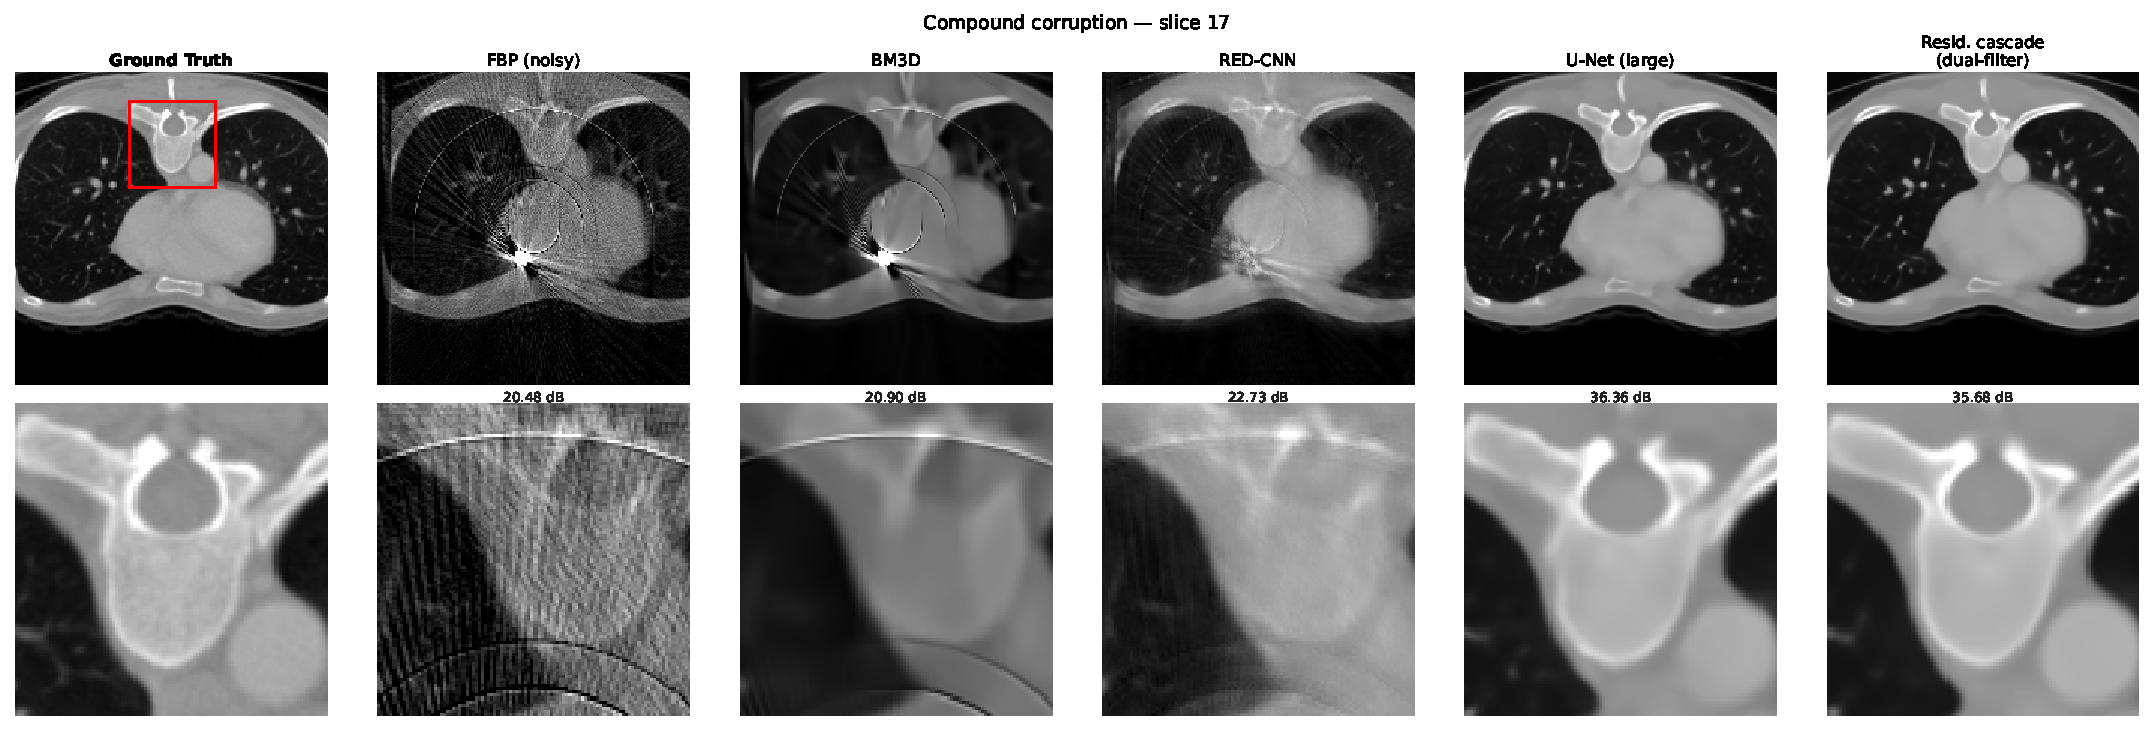
\includegraphics[width=\linewidth]{figures/results/fig_comparison_slice0017.pdf}
    \caption[Cross-method qualitative comparison under compound corruption (slice~17).]{%
        Qualitative comparison on slice~17 under compound corruption (Poisson noise,
        motion, ring, and metal artifacts co-occurring).
        \emph{Top row:} full reconstructions.
        \emph{Bottom row:} magnified crop of the highest-artifact region (red box on
        Ground Truth panel).
        PSNR~(dB) and SSIM are annotated beneath each column.
        BM3D suppresses diffuse noise but leaves structured streaks largely intact.
        RED-CNN removes most of the noise but struggles with metal streak saturation.
        The single-stage U-Net~(large) handles all artifact types effectively.
        The residual cascade with dual-filter input achieves the best visual
        suppression, most clearly visible in the zoomed crop near the streak
        boundaries. Supplementary per-artifact comparisons on additional slices
        are provided in \Cref{app:visuals}.}
    \label{fig:exp_qual_comparison}
\end{figure}

\Cref{fig:exp_qual_cascade} examines the cascade depth effect directly by showing the Stage~1 and Stage~2 outputs of all four cascade variants alongside the ground truth, together with a per-pixel difference map (Stage~2\,$-$\,Stage~1) on a diverging color scale. The difference maps share a common symmetric range across all rows, making the magnitude of Stage~2 corrections directly comparable.

\begin{figure}[!htb]
    \centering
    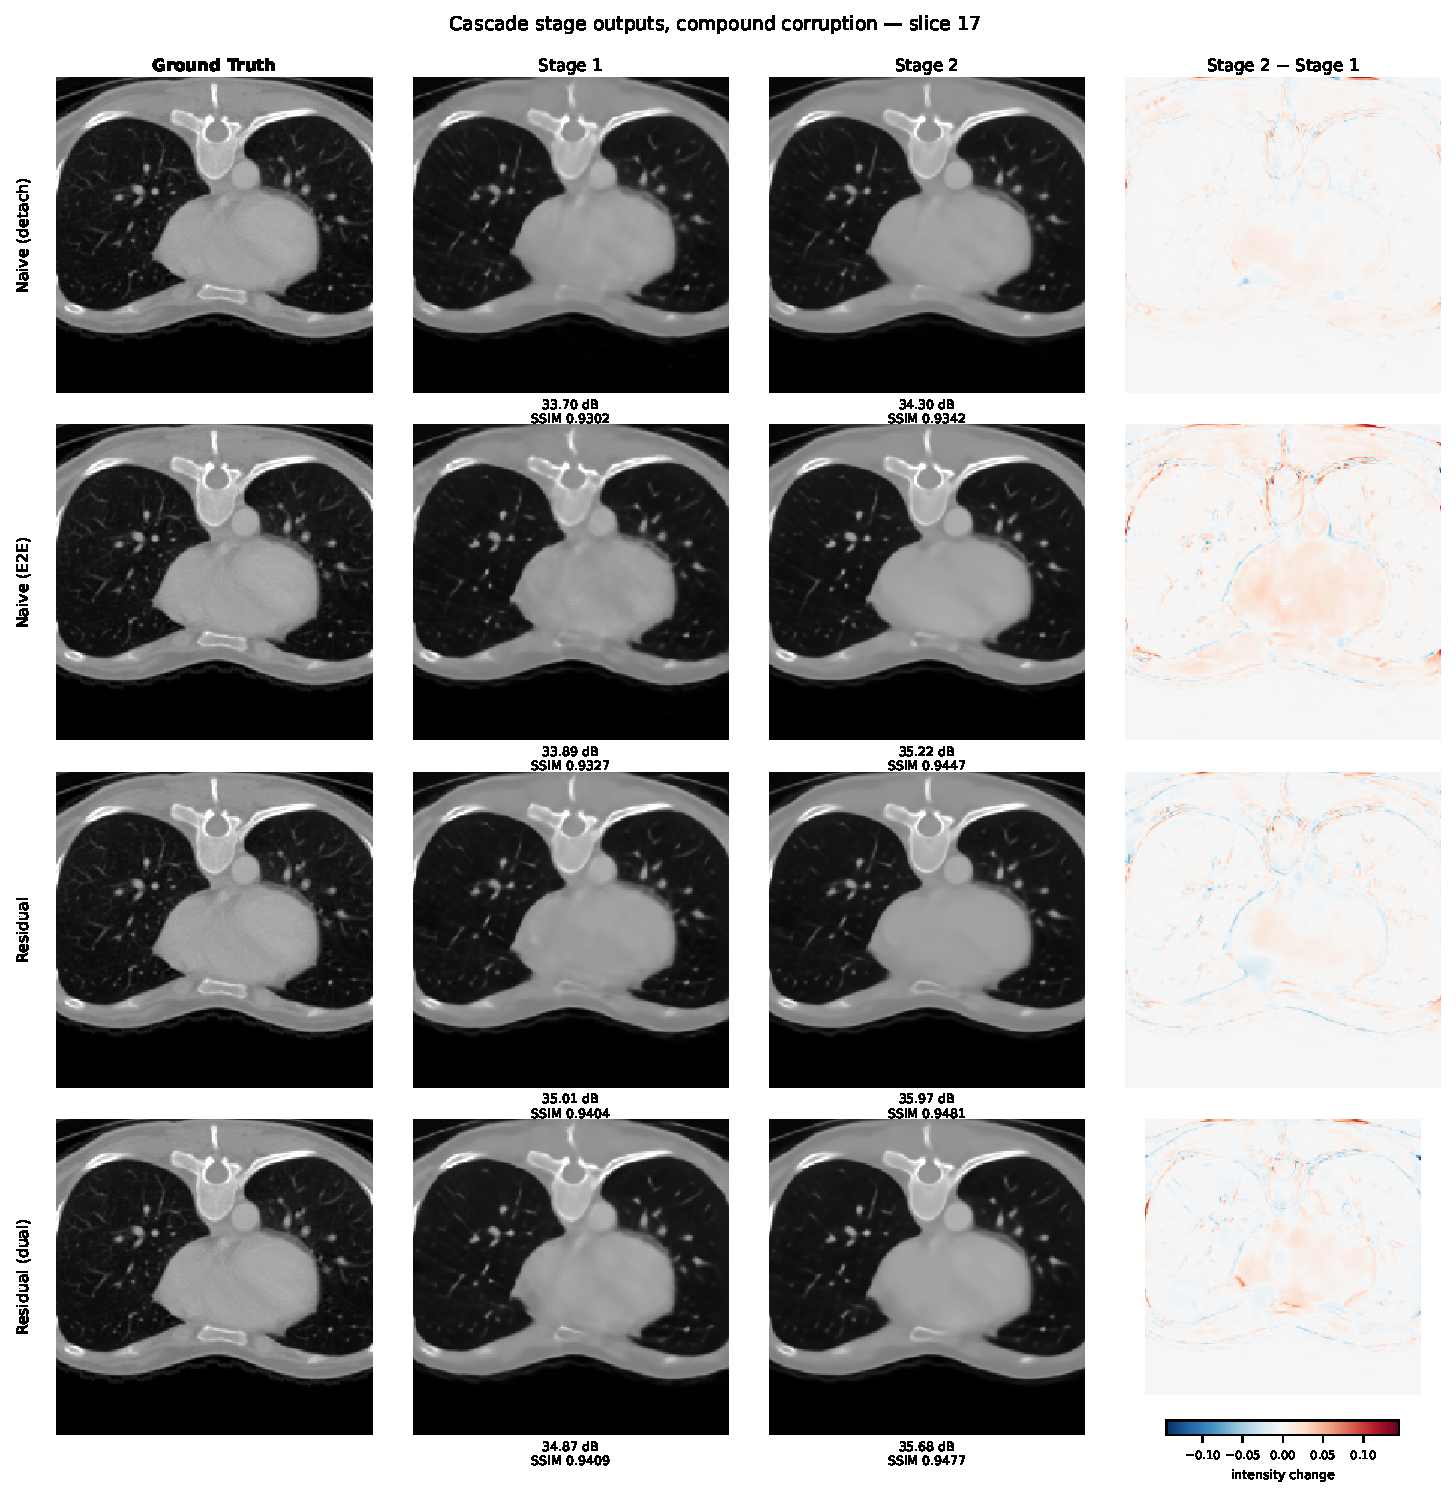
\includegraphics[width=\linewidth]{figures/results/fig_cascade_internals_slice0017.pdf}
    \caption[Cascade stage internals under compound corruption (slice~17).]{%
        Stage-by-stage outputs for all four cascade variants on slice~17 under
        compound corruption.
        \emph{Columns:} ground truth; Stage~1 output (PSNR/SSIM below);
        Stage~2 output (PSNR/SSIM below); per-pixel difference
        Stage~2\,$-$\,Stage~1 on a diverging color scale (blue~=~Stage~2 decreased
        intensity, red~=~increased; shared symmetric scale across all rows).
        In the naive cascade variants the difference maps show diffuse, spatially
        unstructured corrections of low magnitude, consistent with a Stage~2 that
        has received a weak gradient signal and has not learned a specialized
        corrective role.
        In the residual variants the corrections are more concentrated near
        artifact boundaries, with the dual-filter variant showing the most
        structured Stage~2 contribution.}
    \label{fig:exp_qual_cascade}
\end{figure}

The visual results corroborate the quantitative findings in \Cref{tab:exp_cascade}. BM3D reduces diffuse noise but leaves structured artifact signatures largely intact. The learned single-stage U-Net suppresses both noise and physical artifacts effectively, and the gap between the U-Net~(large) and the best cascade is small — visible primarily near metal streak saturation edges in the zoomed crop. The cascade internals figure reveals that the Stage~2 correction is modest across all variants, with the residual dual-filter model showing the most structured improvement, consistent with the $+0.72$\,dB gain reported in \Cref{tab:exp_cascade}.
%%─────────────────────────────────────────────────────────
%% Per-Stage Loss and Gradient Behavior
%%─────────────────────────────────────────────────────────
\section{Per-Stage Loss and Gradient Behavior}
\label{sec:exp_gradient}

To explain why deeper image-domain cascades do not surpass the effective single-network ceiling observed in \Cref{sec:exp_cascade}, the learning dynamics are examined at the level of individual stages.
\Cref{fig:exp_loss_curves} shows representative train and validation loss curves for four model variants, and \Cref{fig:exp_stage_improvement} summarizes the per-stage PSNR progression for the two strongest cascades.

\begin{figure}[!htb]
    \centering
    \begin{minipage}{0.48\linewidth}
        \centering
        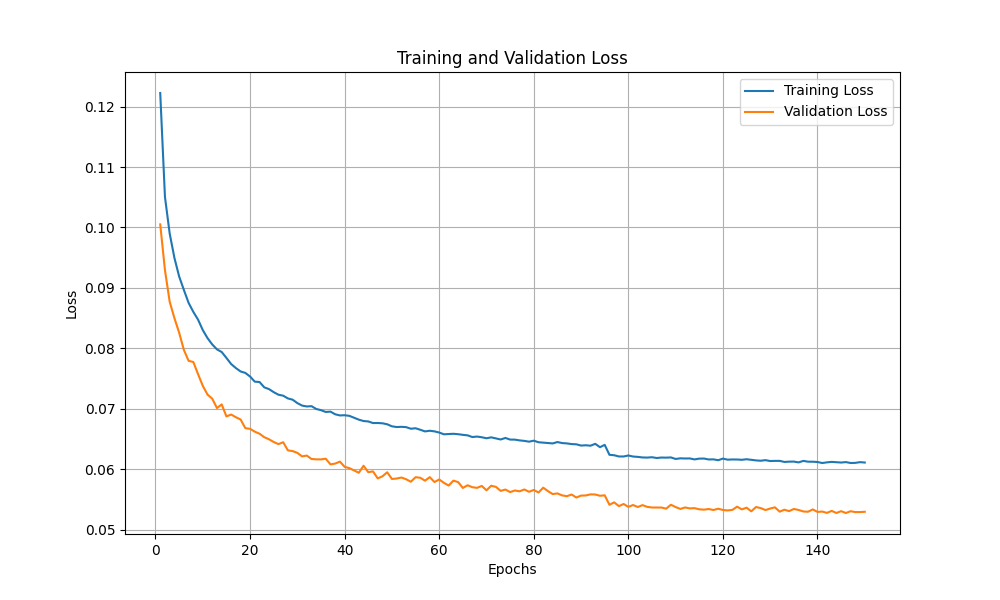
\includegraphics[width=\linewidth]{figures/results/loss_curves_unet_baseline.png}\\
        \footnotesize Single-stage U-Net.
    \end{minipage}\hfill
    \begin{minipage}{0.48\linewidth}
        \centering
        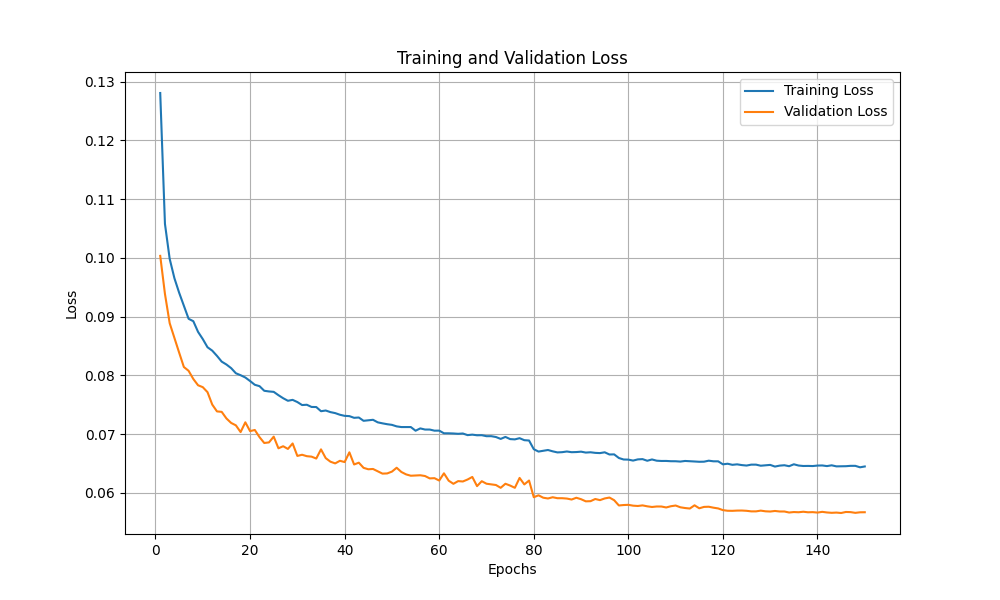
\includegraphics[width=\linewidth]{figures/results/loss_curves_naive_detach.png}\\
        \footnotesize Naive cascade, independent training.
    \end{minipage}\\[1.5ex]
    \begin{minipage}{0.48\linewidth}
        \centering
        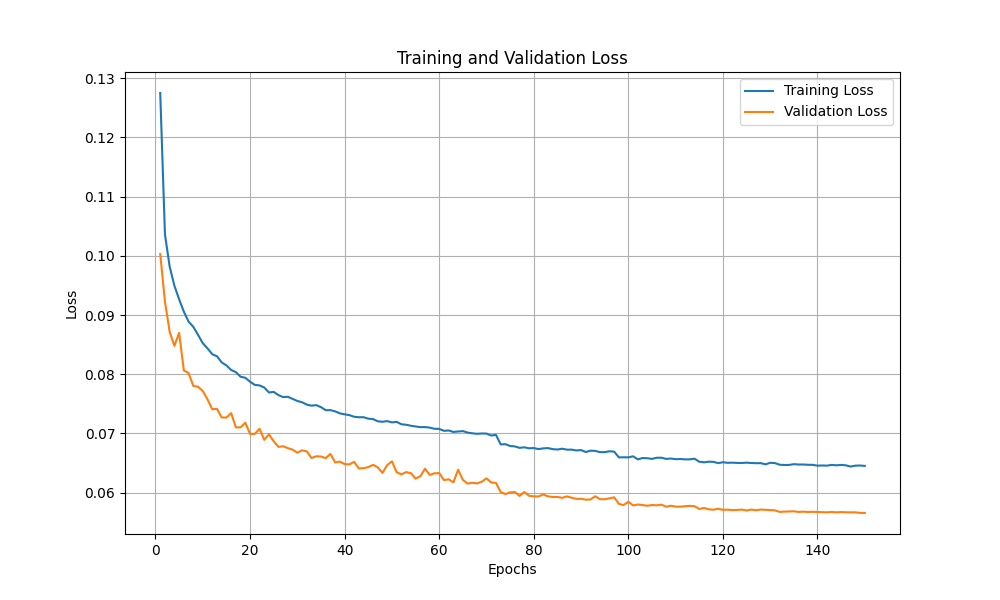
\includegraphics[width=\linewidth]{figures/results/loss_curves_naive_e2e.png}\\
        \footnotesize Naive cascade, end-to-end training.
    \end{minipage}\hfill
    \begin{minipage}{0.48\linewidth}
        \centering
        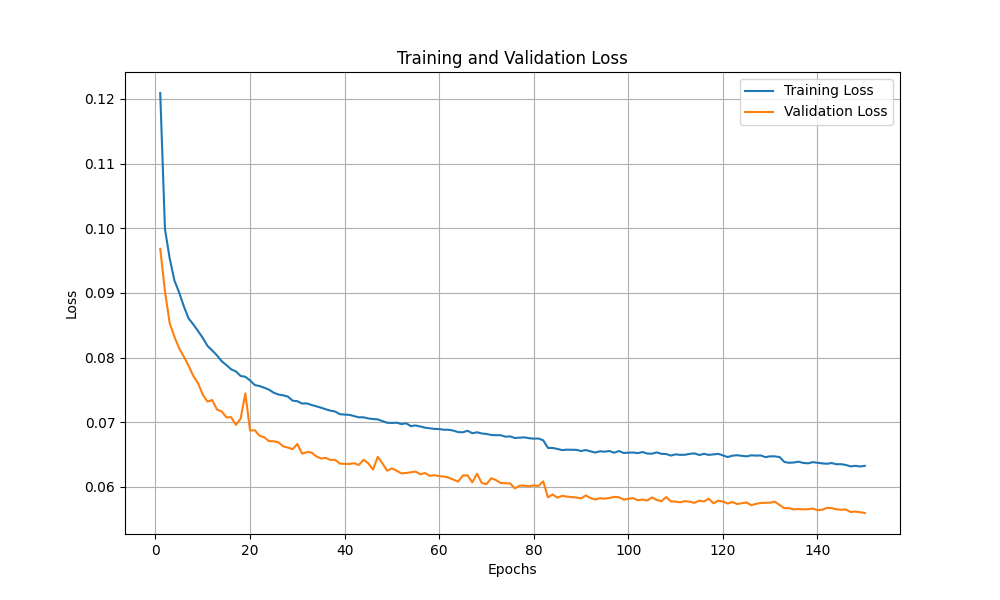
\includegraphics[width=\linewidth]{figures/results/loss_curves_residual_detach.png}\\
        \footnotesize Residual cascade, independent training.
    \end{minipage}
    \caption[Train/validation loss curves for representative variants.]{%
        Per-stage train and validation loss curves for four representative
        models. In all cascade variants, the Stage~1 loss plateaus near the
        same level reached by the single-stage U-Net, indicating that the
        first stage converges to a similar image-domain operating point.
        The Stage~2 loss of the residual cascade settles at a lower value,
        consistent with the smaller-magnitude residual target.}
    \label{fig:exp_loss_curves}
\end{figure}

The loss curves suggest that increased depth alone does not materially alter
the operating point reached by the first stage. Across the cascade variants,
Stage~1 converges to nearly the same loss level as the single-stage U-Net
trained in isolation. This indicates that the first stage already captures
most of the recoverable image-domain improvement under the present protocol,
leaving only a limited residual error for Stage~2 to model.

The residual cascade behaves differently only in the target presented to the
second stage. Because Stage~2 predicts a correction rather than a full clean
image, its optimization target has lower magnitude and is sparser in space.
The lower Stage~2 loss plateau is consistent with this reformulation and
provides one explanation for the stronger performance of the residual
variant in \Cref{tab:exp_cascade}.

\paragraph{Gradient attenuation in the end-to-end cascade.}
The end-to-end variant exhibits a marked attenuation of the Stage~2 learning
signal over training. The trainer logs the mean gradient magnitude for each
stage on the first batch of every epoch. In the small naive end-to-end
cascade, the Stage~2 gradient mean decreases from approximately
$\sim\!10^{-3}$ at initialization to $\sim\!10^{-4}$ within the first five
epochs and continues to decline thereafter, whereas the Stage~1 gradient
remains near the $3\times10^{-4}$ level.

By mid-training, the Stage~1/Stage~2 gradient-magnitude ratio reaches
approximately $3$--$5$. This indicates that the later stage receives a
progressively weaker optimisation signal as Stage~1 approaches its own
converged solution. In this setting, the second stage is not encouraged to
develop a strongly specialized corrective role, which helps explain why the
end-to-end naive cascade does not surpass the independently trained residual
variant in \Cref{tab:exp_cascade}.

\begin{figure}[!htb]
    \centering
    \begin{minipage}{0.48\linewidth}
        \centering
        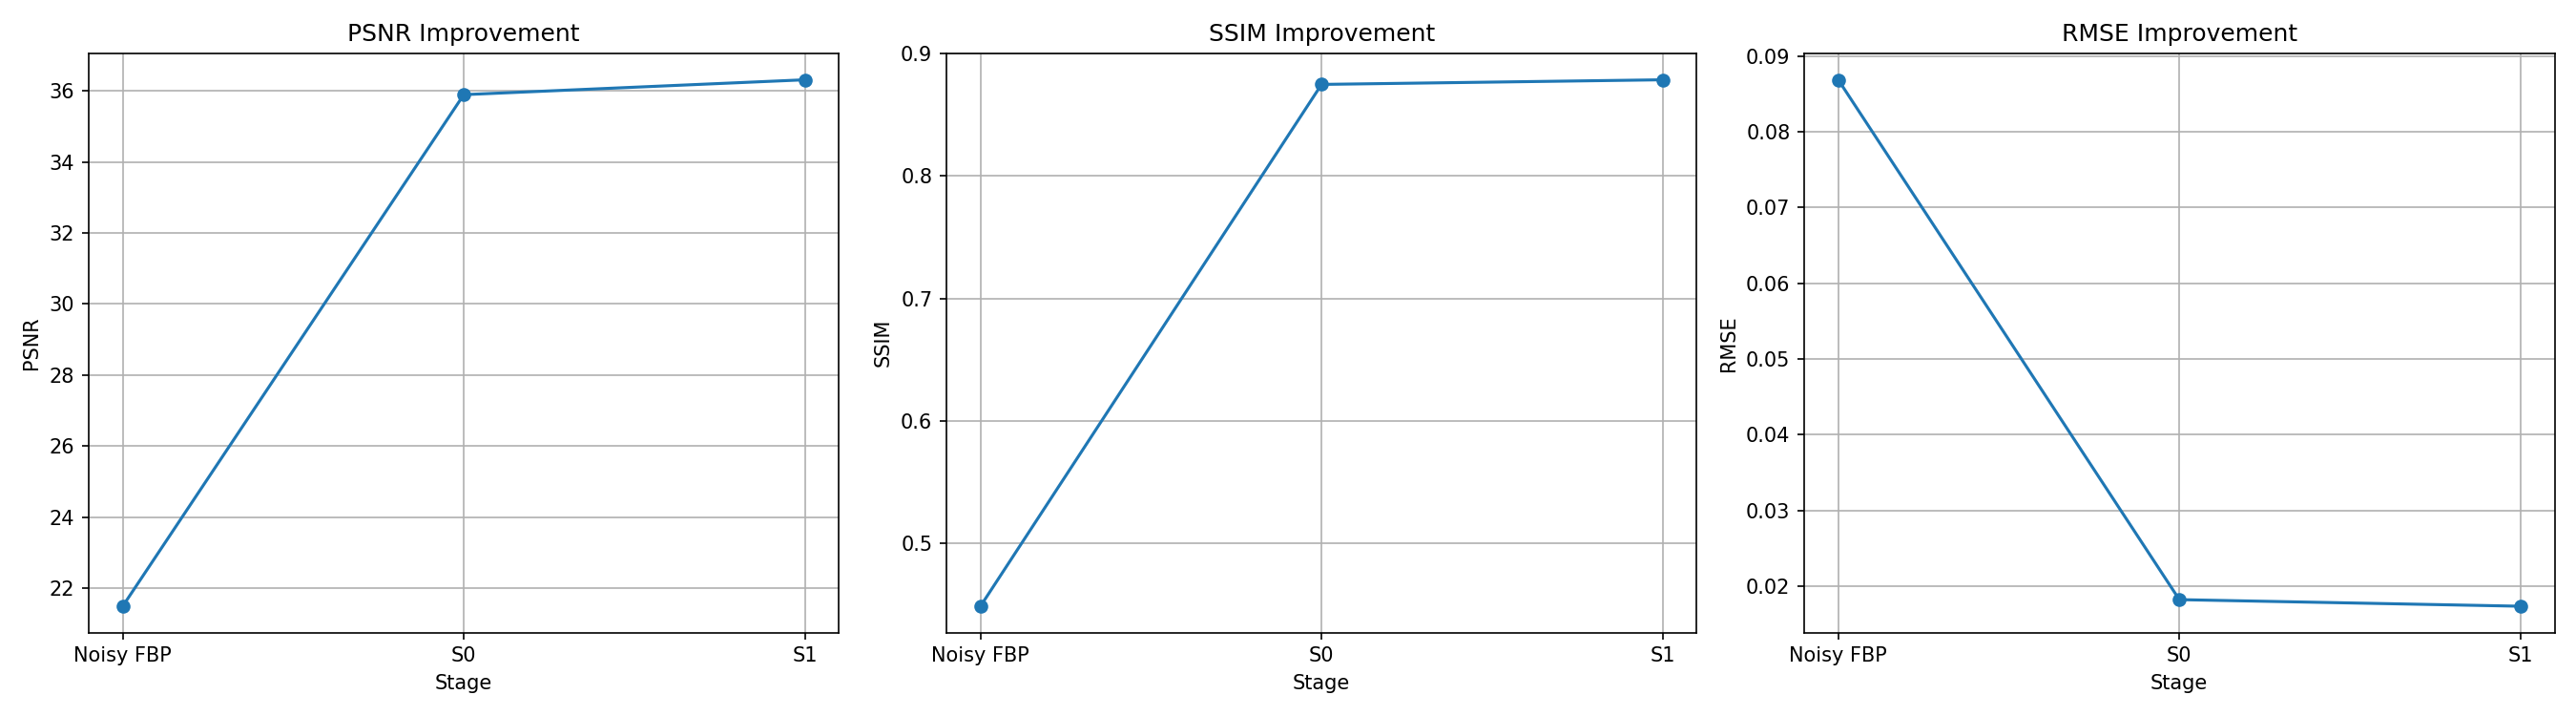
\includegraphics[width=\linewidth]{figures/results/stage_improvement_naive_large.png}\\
        \footnotesize Naive independent cascade (large+large).
    \end{minipage}\hfill
    \begin{minipage}{0.48\linewidth}
        \centering
        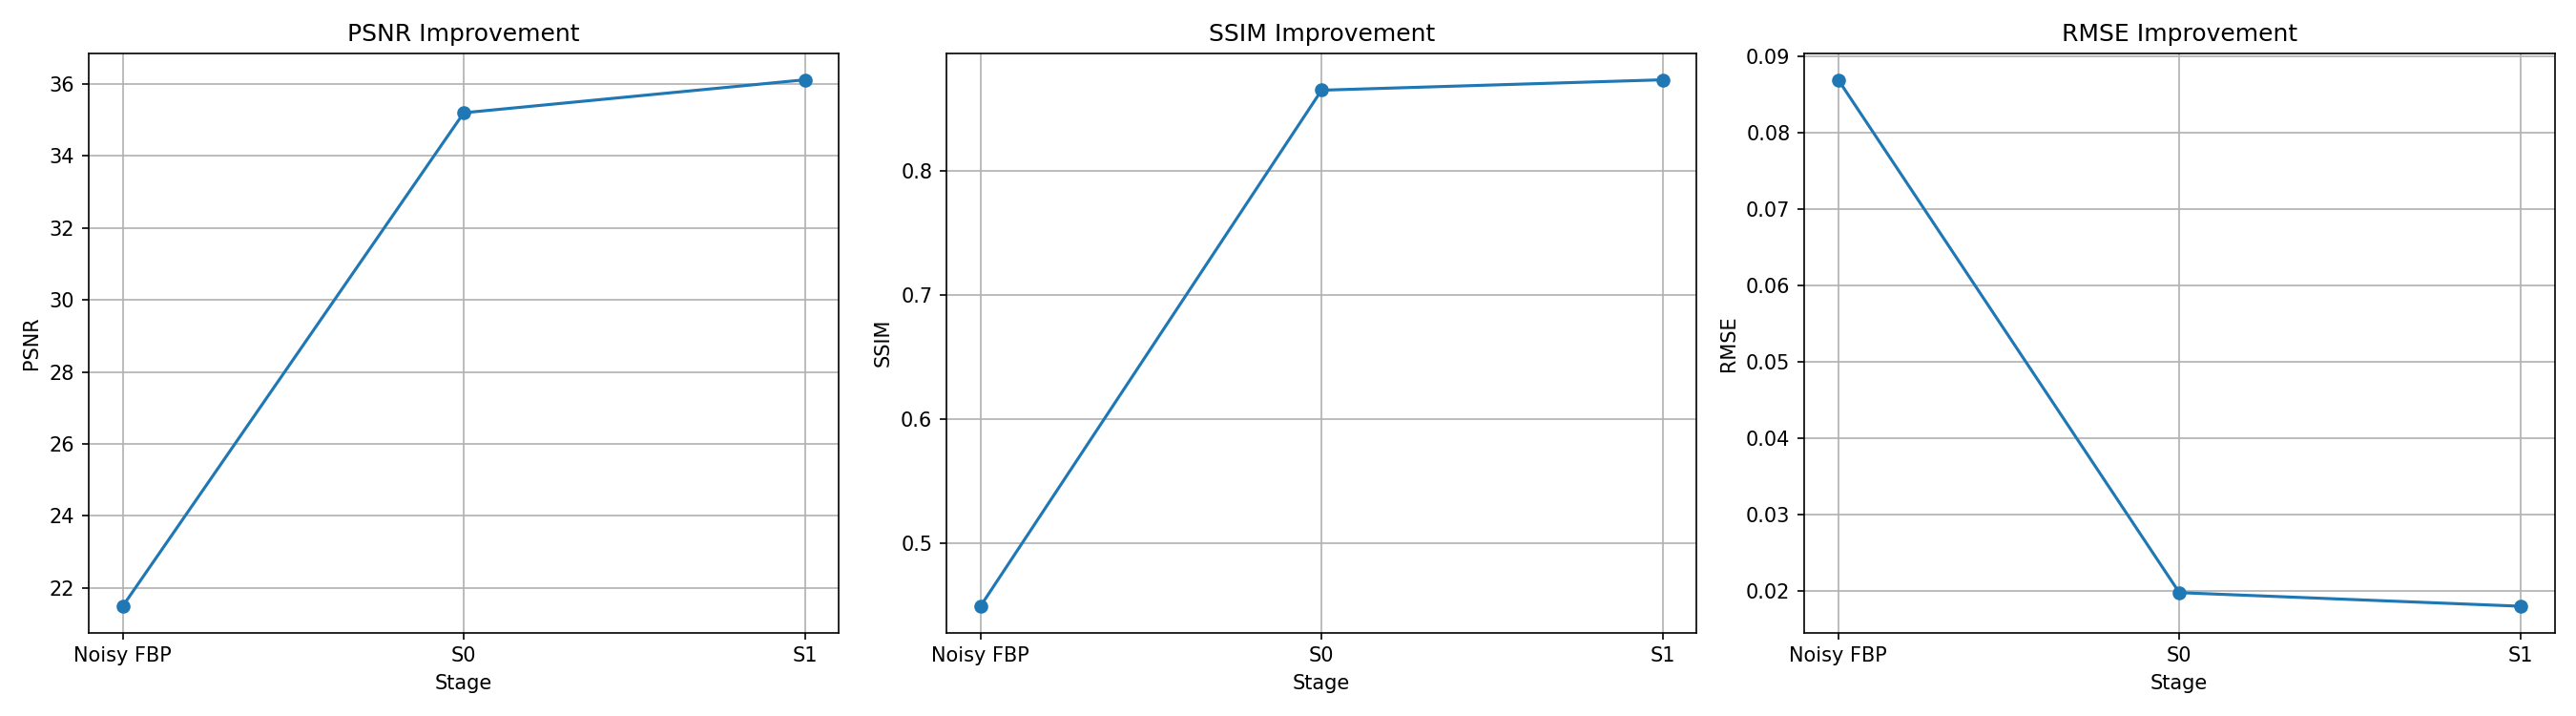
\includegraphics[width=\linewidth]{figures/results/stage_improvement_residual_dual.png}\\
        \footnotesize Residual independent cascade with dual-filter input.
    \end{minipage}
    \caption[Per-stage PSNR progression across the cascade.]{%
        PSNR at the corrupted FBP input, after Stage~1, and after Stage~2
        for the two strongest cascade variants. Most of the total
        improvement is achieved by Stage~1, while the Stage~2 increment is
        comparatively small and approaches the empirical image-domain ceiling
        discussed in \Cref{sec:exp_discussion}.}
    \label{fig:exp_stage_improvement}
\end{figure}

\FloatBarrier
%%─────────────────────────────────────────────────────────
%% Per-Stage Loss and Gradient Behavior
%%─────────────────────────────────────────────────────────
\section{Discussion}
\label{sec:exp_discussion}

\paragraph{An effective image-domain ceiling.}
The results suggest that a single well-designed encoder--decoder operating purely in the image domain already recovers most of the information that is practically recoverable from the FBP reconstruction under the present compound-corruption protocol. The empirical gap between the large single-stage U-Net (\SI{36.11}{\decibel}, SSIM~\num{0.8772}) and the best two-stage cascade in this study (\SI{36.11}{\decibel}, SSIM~\num{0.8738}, residual with dual-filter input) is zero in PSNR and only \num{0.0034} in SSIM. At matched per-stage capacity, the gain of the naive small$+$small cascade over the small single-stage U-Net is only \SI{0.15}{\decibel}. Taken together, these results indicate that simply increasing image-domain depth does not materially extend the attainable reconstruction quality on this protocol.

\paragraph{Why naive additional depth gives little benefit.}
The Stage~1 loss curves in \Cref{fig:exp_loss_curves} plateau at nearly identical values regardless of whether a second stage is attached. This suggests that Stage~1 already converges to essentially the same operating point as the corresponding single-stage model. The residual error that remains after Stage~1 therefore appears to be dominated by information that is not reliably recoverable from the corrupted image-domain input alone, including fine anatomical detail obscured by the combined effects of low photon flux and structured artifacts. Adding a second image-domain network does not change the information content of that input. In the end-to-end variant, this limitation is compounded by the gradient attenuation described in \Cref{sec:exp_gradient}, where the Stage~2 learning signal weakens as Stage~1 approaches convergence.

\paragraph{Residual configuration: empirical improvement and confounded factors.}
The residual cascade produces a consistent empirical improvement over the matched naive independent cascade ($+0.54$\,dB at symmetric small capacity). However, as noted in \Cref{subsec:meth_cascade_variants}, this configuration differs from the naive baseline along three axes simultaneously: the Stage~2 output representation (additive correction rather than direct image prediction), the Stage~2 loss function (residual $\ell^{1}$ plus SSIM plus gradient terms rather than balanced SSIM\,+\,$\ell^{1}$), and the Stage~2 backbone (ResUNet with intra-block shortcuts rather than plain U-Net). Without ablations that isolate each factor, the observed gain cannot be attributed to any single one of these changes.

Residual-learning arguments from image restoration suggest that predicting a lower-magnitude, sparser correction target should be easier to optimize than predicting the full clean image~\cite{Zhang2017}, and the additional gradient loss term is motivated by the metal-streak boundaries that pure SSIM\,/\,$\ell^{1}$ supervision tends to smooth over. Both are plausible contributors, but their individual contributions remain unresolved. The gain from the dual-filter input ($+0.18$\,dB over the standard residual cascade) is more cleanly interpretable, as it is the only difference between those two configurations: Stage~2 receives additional measurement-derived information that was not available in the single-channel case. Together, these modifications allow the cascade to approach the image-domain ceiling more closely, without removing it.

\paragraph{Information versus capacity.}
The asymmetric-capacity probe in \Cref{tab:exp_asym} indicates that final performance is influenced more by the quality of the intermediate representation than by the raw capacity of Stage~2 alone. Moving capacity from Stage~1 to Stage~2 reduces final performance, whereas strengthening Stage~1 and weakening Stage~2 changes the result only modestly. This provides the clearest evidence in the chapter that the second stage is constrained primarily by the residual information available to it rather than by insufficient downstream parameter count.

\paragraph{Per-artifact-count breakdown.}
\Cref{tab:exp_per_artifact} reports mean PSNR stratified by the number of co-occurring physical artifacts ($k = 0,1,2,3$) for all methods evaluated in this chapter. Artifact counts are determined by replaying the per-sample Bernoulli draws with the fixed test seed, yielding $n_{0}=584$, $n_{1}=1525$, $n_{2}=1185$, and $n_{3}=259$ slices in each stratum. All learned methods show a monotonic decrease in PSNR as artifact count increases. At $k=0$ (noise-only), PSNR values are highest for all methods and the spread between cascade variants is most pronounced. Performance differences across cascade formulations remain broadly consistent across strata, following the same ordering observed in the aggregate results of \Cref{tab:exp_cascade}.

\begin{table}[!htb]
    \centering
    \caption[Per-artifact-count PSNR breakdown for all evaluated methods.]{%
        Mean PSNR (dB) on the LoDoPaB-CT test split, stratified by the number of
        physical artifacts co-occurring in each test sample ($k=0$: noise-only;
        $k=1,2,3$: one, two, or three additional physical artifacts beyond the
        inherited Poisson noise). BM3D is not included per stratum as per-slice
        re-evaluation was computationally prohibitive; its aggregate PSNR is
        \SI{22.14}{\decibel}.}
    \label{tab:exp_per_artifact}
    \setlength{\tabcolsep}{5pt}
    \small
    \begin{tabular}{@{}l r r r r r@{}}
        \toprule
        Method & Overall & $k{=}0$ ($n{=}584$) & $k{=}1$ ($n{=}1525$) & $k{=}2$ ($n{=}1185$) & $k{=}3$ ($n{=}259$) \\
        \midrule
        Corrupted FBP               & $21.49$ & $24.08$ & $21.83$ & $20.28$ & $19.14$ \\
        RED-CNN~\cite{Chen2017}     & $27.03$ & $31.67$ & $27.61$ & $24.78$ & $23.19$ \\
        \midrule
        U-Net (small)               & $35.39$ & $39.37$ & $35.85$ & $33.56$ & $31.93$ \\
        \quad Naive indep.          & $35.54$ & $39.01$ & $35.97$ & $33.93$ & $32.48$ \\
        \quad Naive e2e             & $35.85$ & $39.45$ & $36.29$ & $34.16$ & $32.70$ \\
        \quad Residual              & $35.93$ & $39.56$ & $36.32$ & $34.27$ & $32.84$ \\
        \quad Residual + dual-filter& $36.11$ & $\mathbf{39.91}$ & $\mathbf{36.62}$ & $34.32$ & $32.63$ \\
        \midrule
        U-Net (large)               & $36.11$ & $39.64$ & $36.55$ & $\mathbf{34.47}$ & $\mathbf{32.99}$ \\
        \bottomrule
    \end{tabular}
\end{table}

\paragraph{Scope of the claim.}
These conclusions are based on depth-two cascades evaluated on LoDoPaB-CT under the specific compound-corruption protocol of \Cref{sec:meth_overview}. They should not be generalized automatically to architectures with explicit sinogram-domain processing, to datasets with substantially different anatomy or dose conditions, or to corruption regimes in which the post-Stage~1 residual retains richer exploitable structure. Even so, the dual-filter result points to the most promising direction observed in this study: the second stage becomes more useful when it receives information that is not already compressed into the Stage~1 output. A natural extension is therefore to combine image-domain refinement with an additional upstream branch that operates before reconstruction, as discussed in \Cref{chap:conclusion}.        % Chapter 4: Experiments and Results
\cleardoublepage
\chapter{Conclusion and Outlook}
\label{chap:conclusion}

\section{Summary of Findings}
\label{sec:conc_summary}

This thesis investigated how architectural depth in image-domain cascaded encoder--decoder networks affects \gls{ct} restoration quality under compound corruption. Two contributions support this study. First, \Cref{sec:meth_overview} introduced a physics-informed multi-artifact sinogram corruption protocol that combines low-dose Poisson quantum noise with three independently gated physical artifact models: sinogram-domain motion, per-column ring offsets, and forward-projected metal masks with photon-starvation clipping. The protocol is implemented as a reproducible CPU-side dataset transform compatible with the \gls{lodopab} train/validation/test split. Second, \Cref{chap:experiments} presented a systematic comparison of independent-stage, end-to-end, and residual image-domain cascades against classical and learned single-stage baselines, together with per-stage loss and gradient analyzes used to interpret observed behavior.

The main empirical finding is that, under the compound corruption studied here, a single well-designed image-domain encoder--decoder already operates close to an effective performance ceiling that two-stage cascades do not surpass by depth alone. Concretely:

\begin{itemize}
    \item The large single-stage U-Net achieves \SI{36.11}{\decibel} PSNR and \num{0.8772} SSIM on the LoDoPaB-CT test split under the full compound-corruption distribution.
    \item At matched small per-stage capacity, the gain over the small single-stage U-Net increases monotonically across the cascade variants, from naive independent training to residual prediction to residual prediction with dual-filter input ($+0.15 \to +0.54 \to +0.72$\,dB).
    \item The strongest small-capacity cascade, namely the residual variant with dual-filter conditioning, matches the PSNR of the large single-stage U-Net while remaining slightly below it in SSIM.
    \item The end-to-end cascade exhibits progressive attenuation of the Stage~2 learning signal as Stage~1 approaches convergence, which helps explain why end-to-end coupling does not outperform the independently trained residual formulation.
    \item The asymmetric-capacity probe indicates that the second stage is constrained more by the residual information available to it than by its parameter count alone.
\end{itemize}

This is best interpreted as an architectural ceiling result rather than a negative one. The central conclusion is not simply that deeper image-domain cascades help little, but that additional depth becomes useful only when the later stage receives information that is not already compressed into the Stage~1 output.

\section{Author's Contributions}
\label{sec:conc_originality}

Following the \gls{lme} thesis guidelines (§1.7), the original contributions of this thesis are stated explicitly here. The author designed and implemented the physics-informed multi-artifact corruption protocol of \Cref{sec:meth_overview}, including the metal forward-projection library and the photon-starvation clipping mechanism of \Cref{eq:meth_metal_starvation}. The author also implemented the cascaded U-Net training framework, the dual-filter alternative-input scheme of \Cref{eq:meth_alt_input}, the residual-cascade loss formulation of \Cref{eq:meth_loss_residual}, the baseline pipelines (\gls{bm3d}, single-stage U-Net, and RED-CNN), and the full experimental and reporting workflow. The U-Net backbone follows \cite{Ronneberger2015}, while the residual-prediction principle follows prior work such as DnCNN \cite{Zhang2017} and ResNet \cite{He2016}; in this thesis these established ideas are adapted to the specific cascade comparison studied here. The LoDoPaB-CT dataset and its inherited low-dose sinograms are due to Leuschner et al.~\cite{Leuschner2021}.

\section{Limitations}
\label{sec:conc_limitations}

Four limitations bound the conclusions of this thesis.

\paragraph{Single dataset and simulated corruption.}
All experiments were conducted on \gls{lodopab}, whose ground-truth images are themselves reconstructed from clinical scan data rather than acquired as physical phantom references, and whose low-dose Poisson noise was simulated at $N_0=\num{4096}$. The three physical artifacts considered here were also injected synthetically. Although the artifact models are grounded in the physical literature~\cite{LuMackie2002, Mao2007, Sijbers2004, Prell2009, Gjesteby2016}, the present protocol does not capture effects such as polyenergetic beam hardening, scatter, or non-rigid motion. The ceiling result should therefore be re-tested on projection data that are closer to clinical acquisition.

\paragraph{Independent artifact sampling.}
The three artifact classes are gated independently through Bernoulli sampling in \Cref{eq:meth_compound}. Clinically meaningful correlations between artifact types are therefore not modeled. A conditional sampler informed by scan context or indication would provide a more realistic corruption distribution.

\paragraph{Cascade depth limited to two.}
The experiments in this thesis are limited to two-stage cascades. It therefore remains open whether deeper cascades would provide additional benefit if new information were injected at each stage. The gradient attenuation observed in \Cref{sec:exp_gradient} suggests that naive end-to-end scaling is unlikely to help under the present protocol, but a controlled three-stage study would be needed to test this directly.

\paragraph{Image-domain scope.}
The architectural conclusion reached here applies specifically to cascades that operate in the image domain after filtered backprojection. It should not be generalized automatically to dual-domain systems, learned reconstruction operators, or iterative methods that can exploit sinogram information unavailable to the present models.

\section{Future Work}
\label{sec:conc_future}

The most natural next step is to break the effective image-domain ceiling identified in \Cref{sec:exp_discussion} by supplying later stages with genuinely new information. Two directions emerge directly from the present results.

\paragraph{Sinogram-domain refinement.}
A lightweight network operating on the corrupted sinogram $\tilde{\mathbf{s}}$, followed by reconstruction and fusion with the image-domain Stage~1 output, would give Stage~2 access to information that is not derivable from $\hat{\mathbf{x}}_1$ alone. This is the natural extension suggested by the dual-filter result: the second stage became more useful precisely when it was given an alternative view of the same corrupted measurement.

\paragraph{Projection-domain validation on other datasets.}
Repeating the cascade study on projection-domain datasets with different scanner geometries and anatomy would test whether the image-domain ceiling observed here is specific to LoDoPaB-CT or reflects a more general limitation of post-reconstruction restoration under compound corruption.

\paragraph{Learned reconstruction operators.}
A complementary direction is to relax the fixed FBP operator and allow part of the reconstruction step itself to be learned, for example through learned filtered backprojection or a lightly unrolled iterative scheme. This would allow the model to redistribute capacity across reconstruction and restoration rather than restricting all adaptation to post-reconstruction image processing.

\paragraph{Beyond two stages with information injection.}
A controlled study of three-stage cascades, with additional information injected at every stage, would help distinguish whether the observed ceiling is fundamentally per-stage or per-cascade. On the basis of the present results, residual coupling with explicit information injection would be the most promising formulation to scale beyond two stages.         % Chapter 5: Conclusion and Outlook
\cleardoublepage

\appendix
\cleardoublepage
\chapter{Additional Visual Results}
\label{app:visuals}

\Cref{fig:exp_qual_comparison,fig:exp_qual_cascade} in the main text (\Cref{sec:exp_qualitative}) show the cross-method comparison and the cascade stage internals for slice~17 under compound corruption. This appendix provides supplementary per-artifact qualitative comparisons on two additional test slices (3161 and~981) using the same figure format: a full reconstruction row and a magnified crop of the highest-artifact region, with PSNR~(dB) and SSIM annotated beneath each column. All figures show: Ground Truth~$|$ FBP~(noisy)~$|$ BM3D~$|$ RED-CNN~$|$ U-Net~(large)~$|$ Residual cascade~(dual-filter).

\section*{Slice 3161}

\begin{figure}[!htbp]
    \centering
    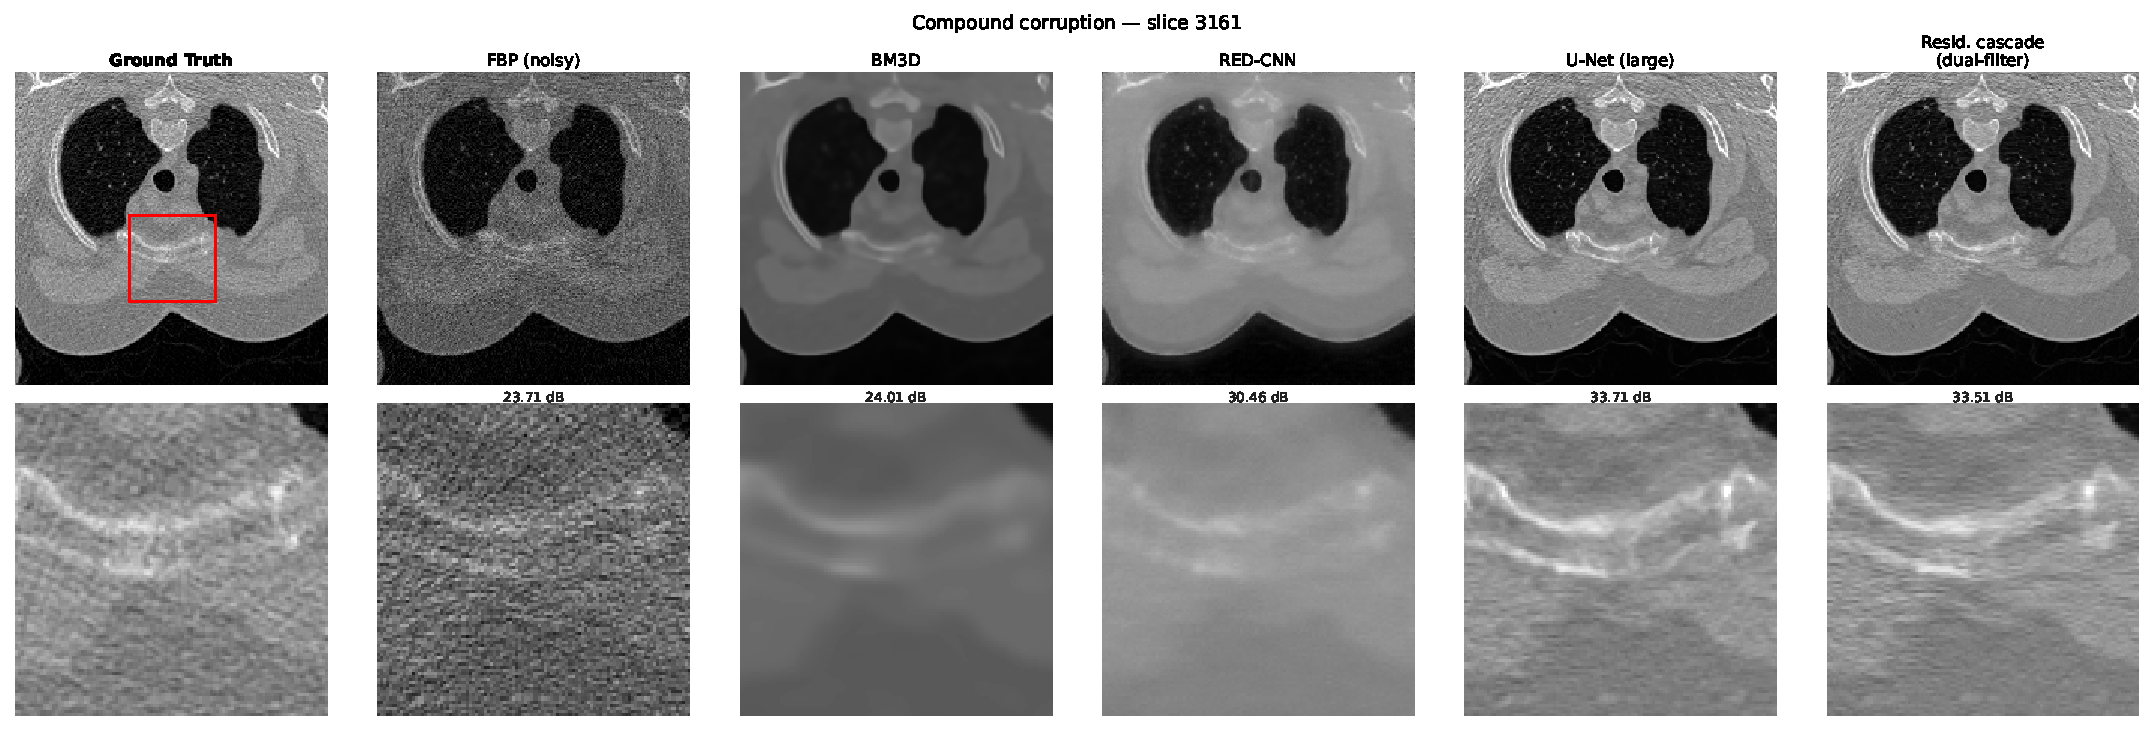
\includegraphics[width=\linewidth]{figures/results/fig_app_noise_only_slice3161.pdf}
    \caption[Slice~3161: noise-only condition.]{%
        Slice~3161, noise-only (low-dose Poisson noise, no physical artifacts).
        The learned models recover soft-tissue contrast suppressed by quantum noise;
        BM3D partially reduces noise but over-smooths fine structure.}
    \label{fig:app_qual_noise_3161}
\end{figure}

\begin{figure}[!htbp]
    \centering
    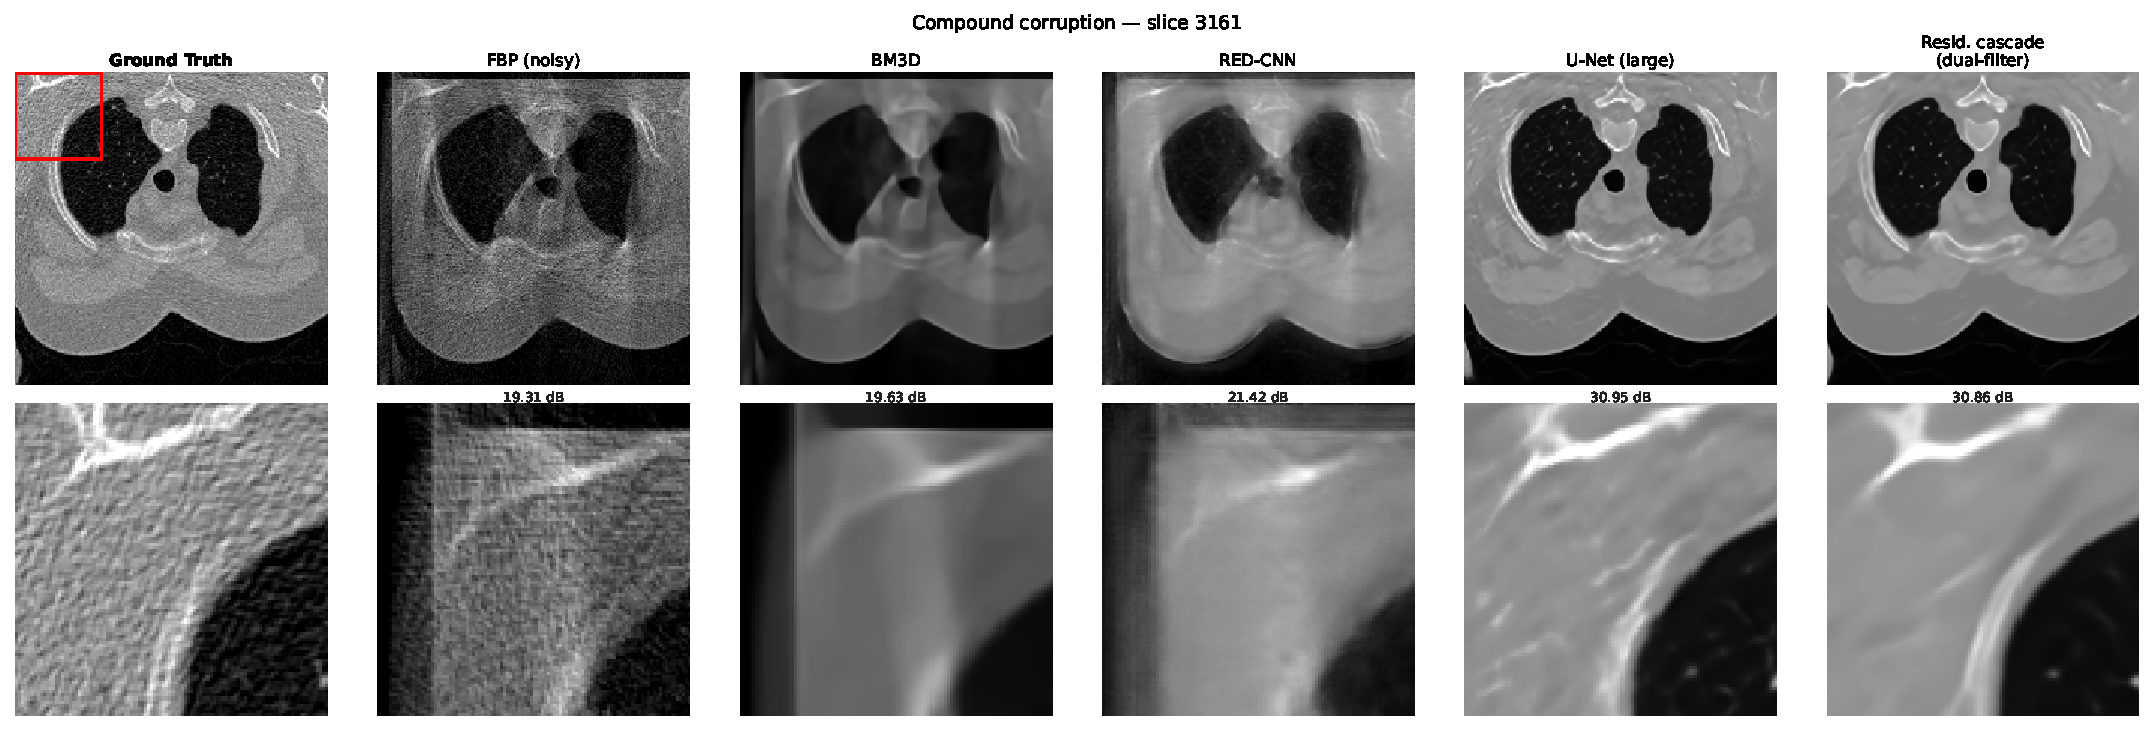
\includegraphics[width=\linewidth]{figures/results/fig_app_motion_slice3161.pdf}
    \caption[Slice~3161: motion artifact condition.]{%
        Slice~3161 with added respiratory motion artifacts (periodic sinogram shift,
        amplitude 10--20\,bins, 0.5--1.5 breathing cycles).
        Motion introduces edge blurring and ghosting visible in the zoomed crop;
        BM3D and RED-CNN partially mitigate noise but cannot resolve the motion
        inconsistency. Both U-Net variants substantially suppress the blurring.}
    \label{fig:app_qual_motion_3161}
\end{figure}

\begin{figure}[!htbp]
    \centering
    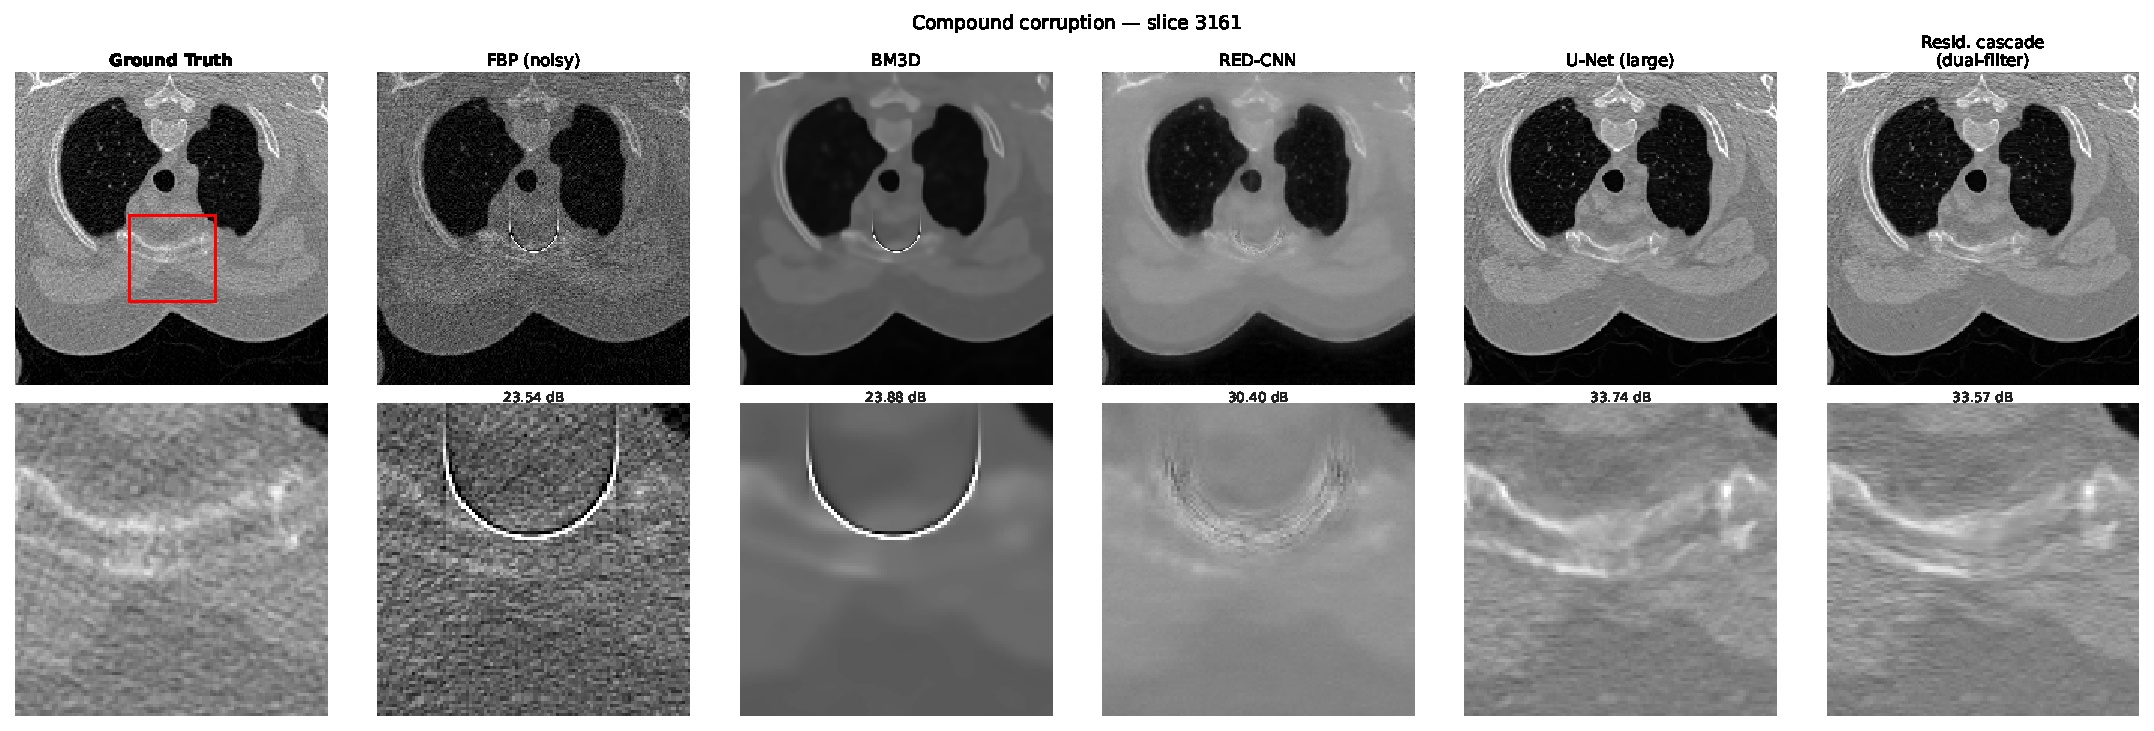
\includegraphics[width=\linewidth]{figures/results/fig_app_ring_slice3161.pdf}
    \caption[Slice~3161: ring artifact condition.]{%
        Slice~3161 with added detector ring artifacts (1--5 columns, gain error
        5--50\,\%). Concentric ring bands are visible in the FBP reconstruction;
        the learned models suppress these effectively while retaining tissue detail.}
    \label{fig:app_qual_ring_3161}
\end{figure}

\begin{figure}[!htbp]
    \centering
    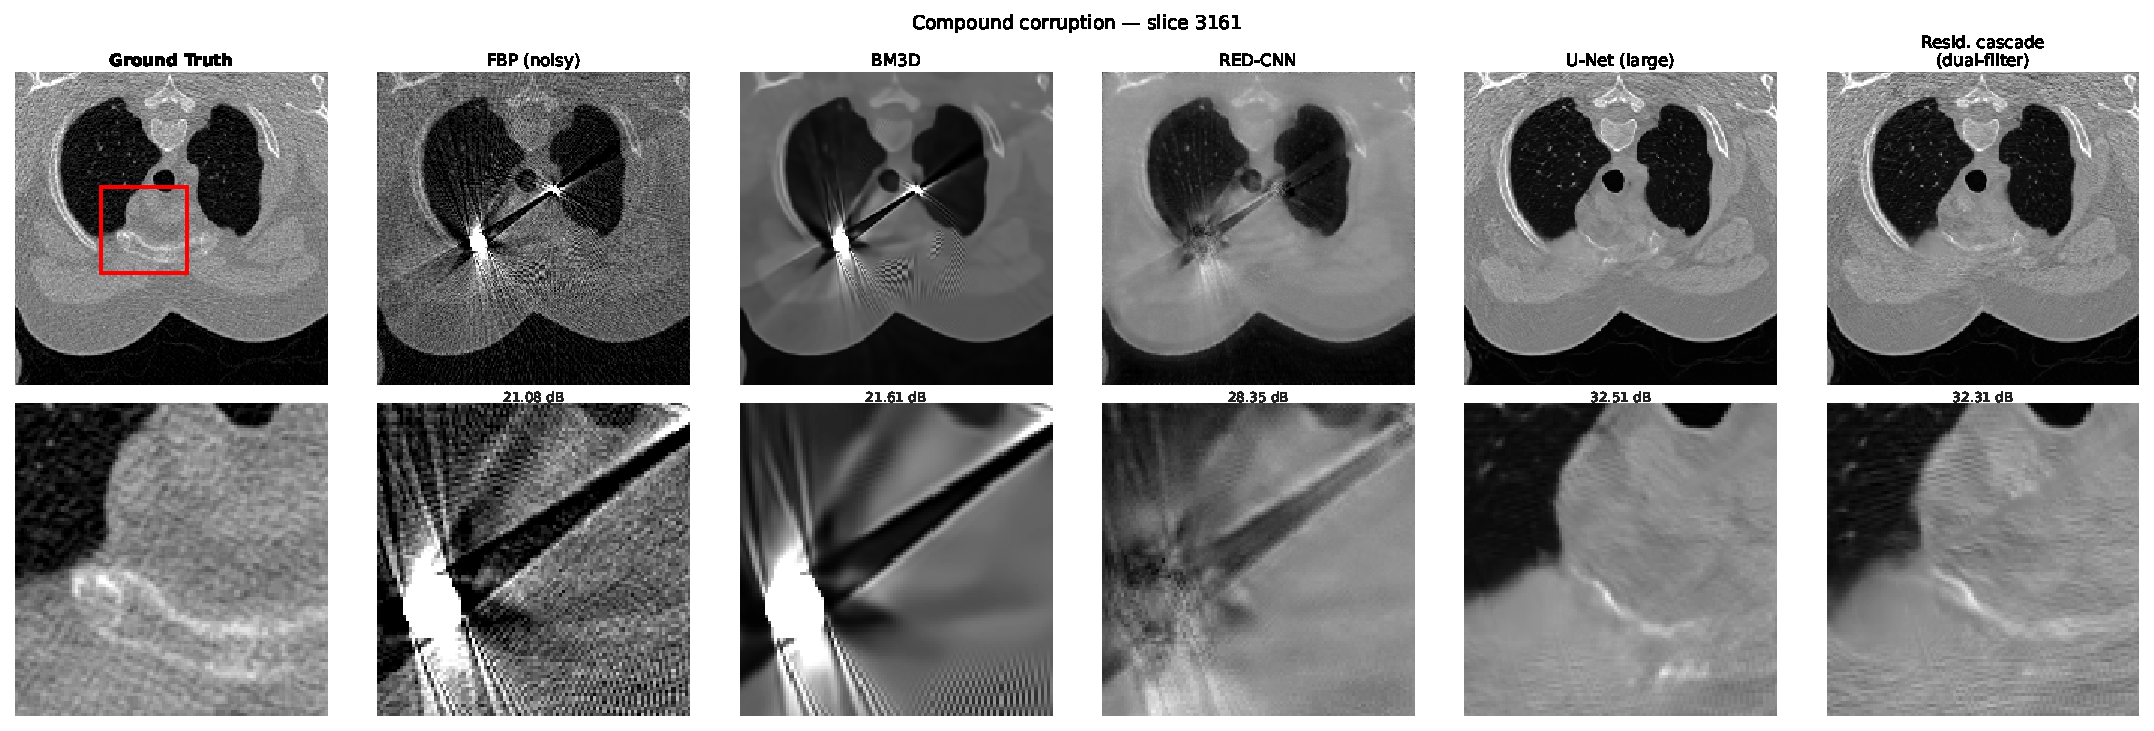
\includegraphics[width=\linewidth]{figures/results/fig_app_metal_slice3161.pdf}
    \caption[Slice~3161: metal artifact condition.]{%
        Slice~3161 with added metal implant artifacts (1--2 implants, scale
        0.10--0.30, photon-starvation clipping). Bright and dark saturation streaks
        are prominent in the FBP; the residual cascade with dual-filter input
        achieves the strongest streak suppression, visible in the zoomed crop.}
    \label{fig:app_qual_metal_3161}
\end{figure}

\begin{figure}[!htbp]
    \centering
    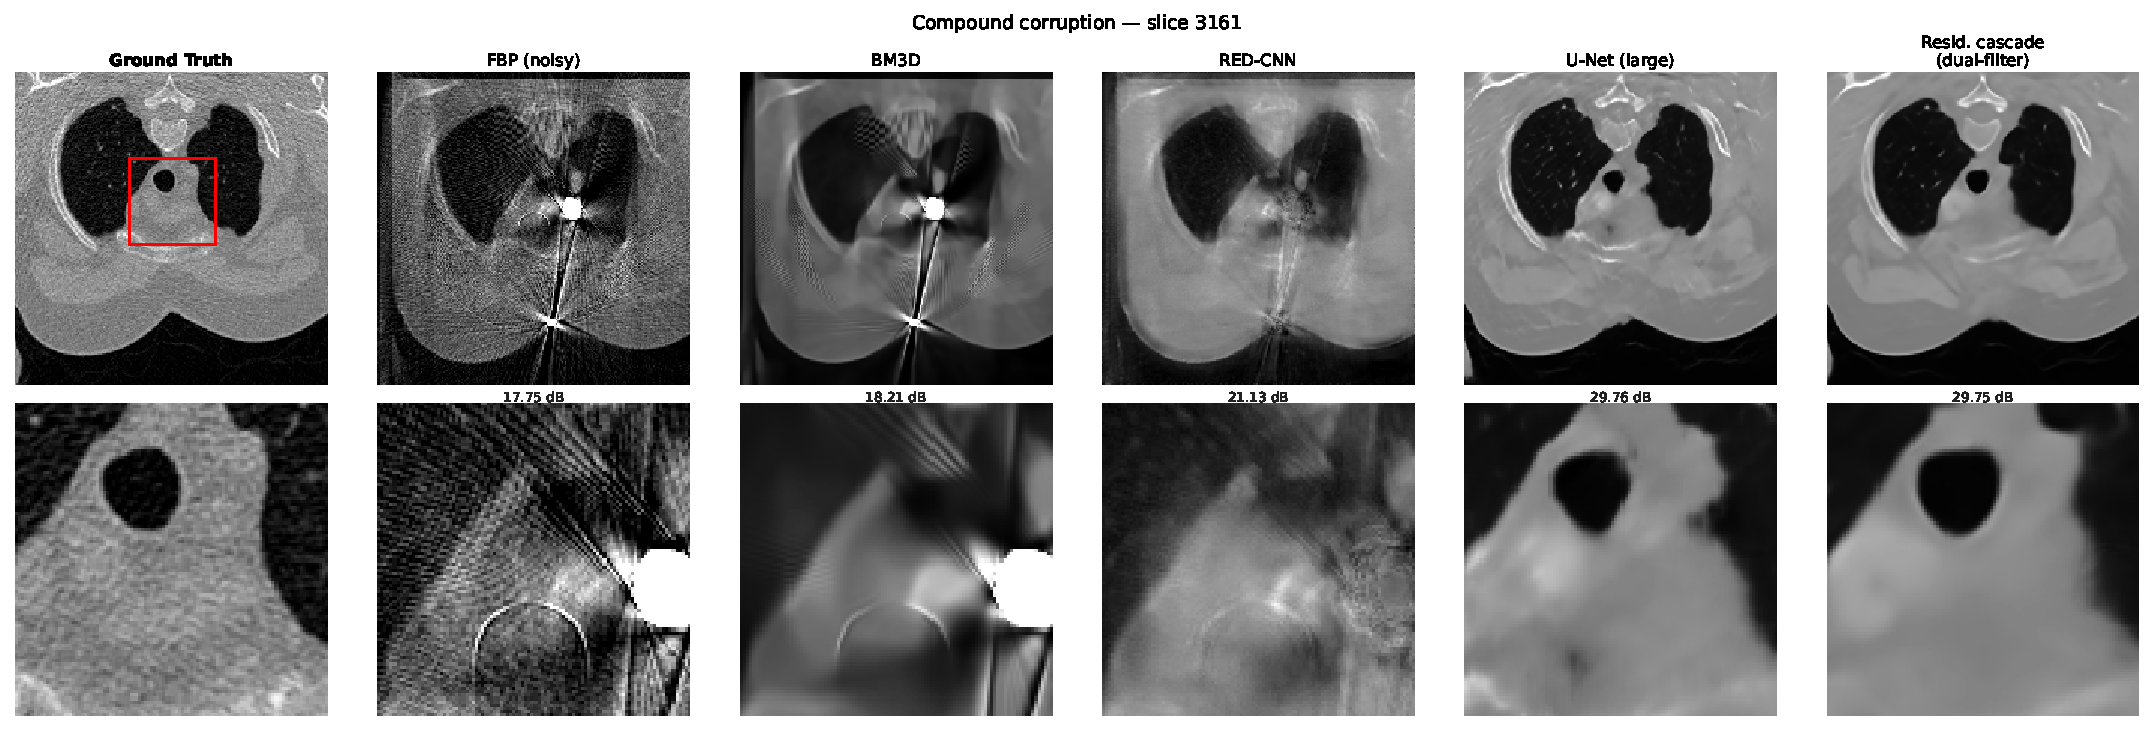
\includegraphics[width=\linewidth]{figures/results/fig_app_compound_slice3161.pdf}
    \caption[Slice~3161: compound corruption condition.]{%
        Slice~3161 under compound corruption (all three physical artifact types
        co-occurring simultaneously with Poisson noise). This is the hardest
        corruption regime evaluated in this thesis. The zoomed crop highlights
        the combined streak and ring pattern; the residual dual-filter cascade
        provides the most complete suppression.}
    \label{fig:app_qual_compound_3161}
\end{figure}

\section*{Slice 981}

\begin{figure}[!htbp]
    \centering
    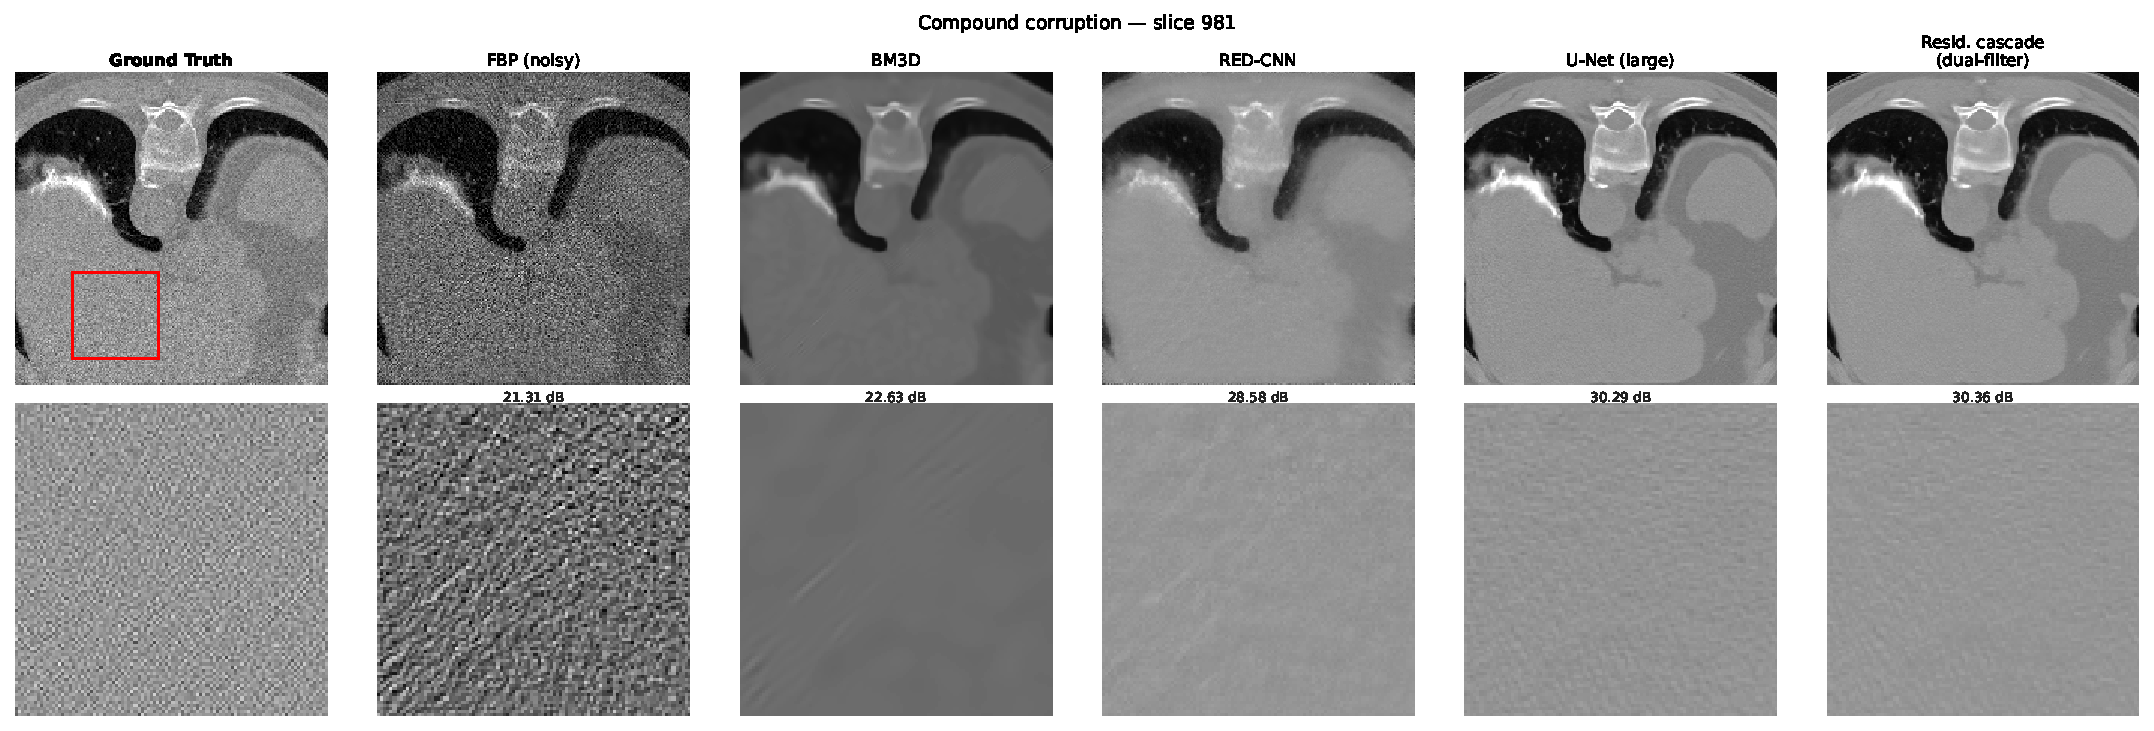
\includegraphics[width=\linewidth]{figures/results/fig_app_noise_only_slice0981.pdf}
    \caption[Slice~981: noise-only condition.]{%
        Slice~981, noise-only condition (low-dose Poisson noise only, no physical
        artifacts). All learned methods recover soft-tissue contrast suppressed by
        quantum noise; the residual dual-filter cascade and the large U-Net are
        visually indistinguishable at this corruption level, consistent with
        the per-artifact PSNR breakdown in \Cref{tab:exp_per_artifact}.}
    \label{fig:app_qual_noise_981}
\end{figure}

\begin{figure}[!htbp]
    \centering
    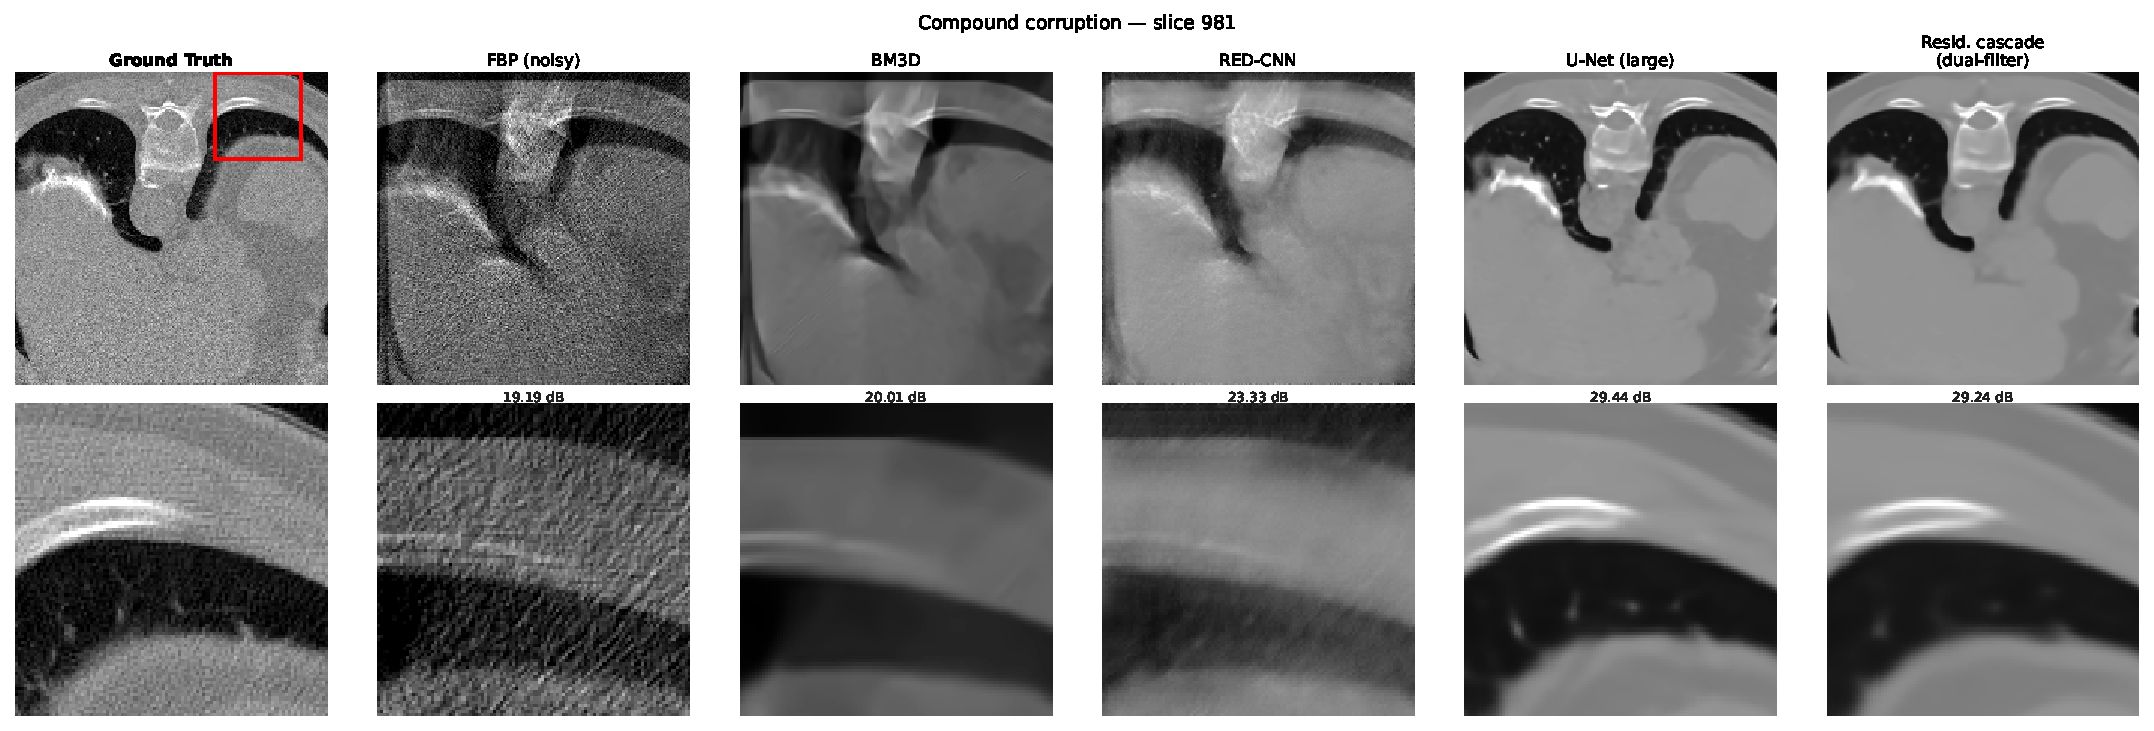
\includegraphics[width=\linewidth]{figures/results/fig_app_motion_slice0981.pdf}
    \caption[Slice~981: motion artifact condition.]{%
        Slice~981 with added respiratory motion artifacts (periodic sinogram shift,
        amplitude 10--20\,bins, 0.5--1.5 breathing cycles).
        The characteristic edge-blurring and double-contour effect is visible along
        lung-tissue boundaries in the corrupted FBP. Both U-Net variants suppress
        the blurring effectively; BM3D and RED-CNN partially reduce diffuse noise
        but leave the sinogram-domain inconsistency largely unresolved.}
    \label{fig:app_qual_motion_981}
\end{figure}

\begin{figure}[!htbp]
    \centering
    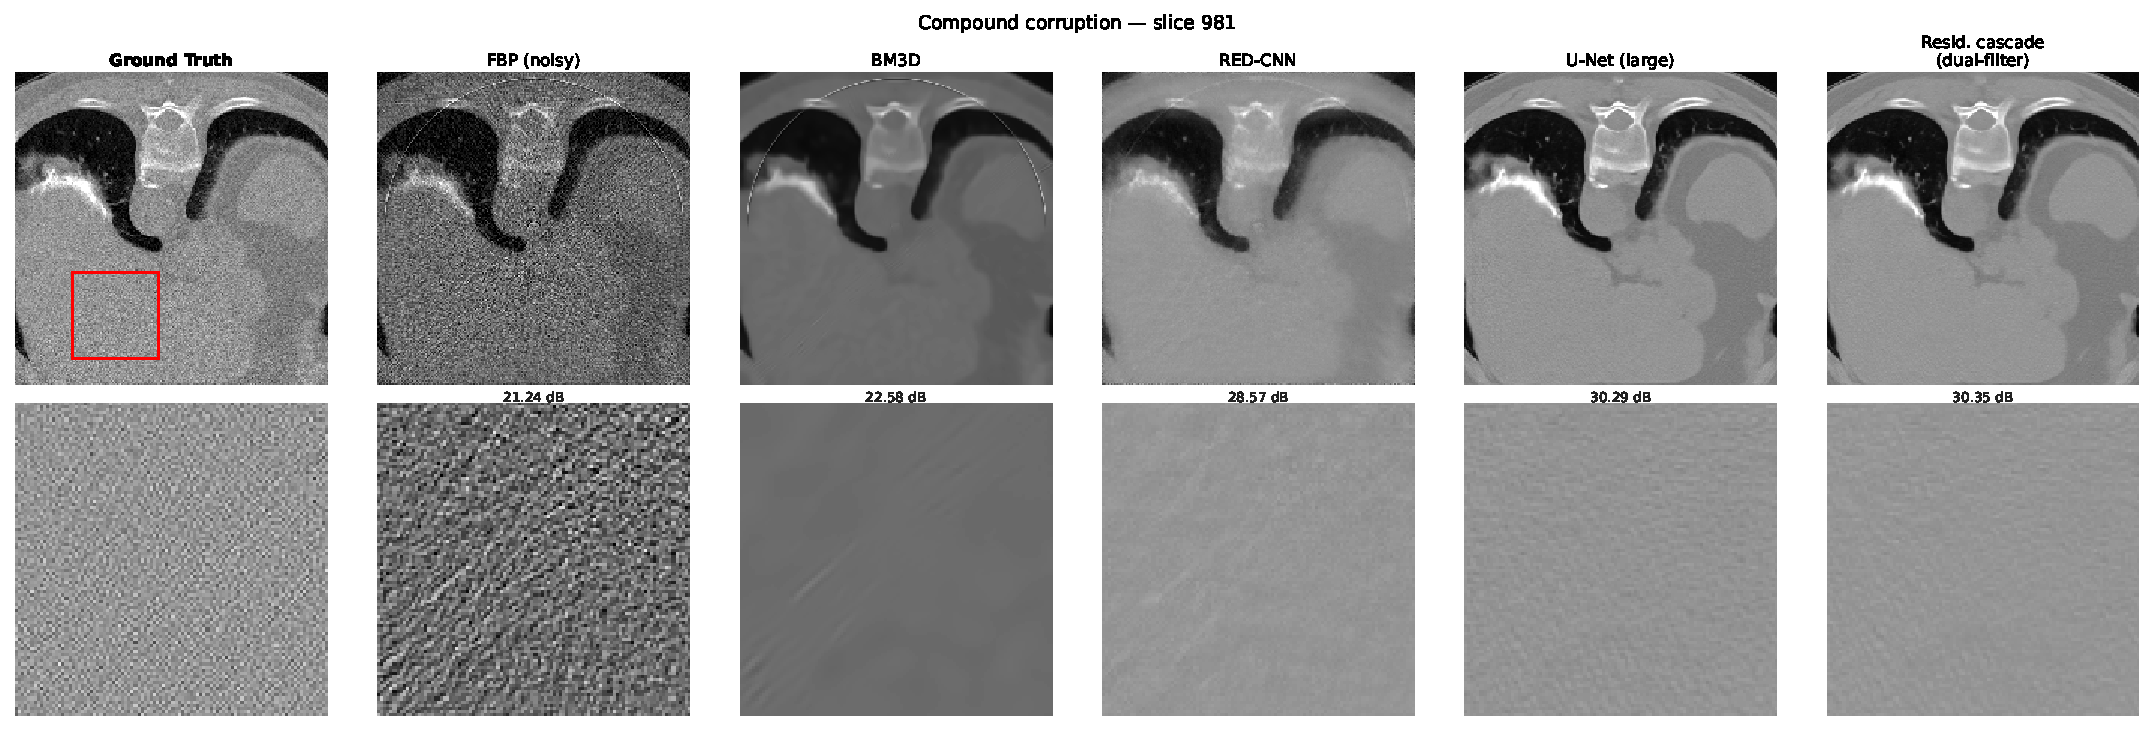
\includegraphics[width=\linewidth]{figures/results/fig_app_ring_slice0981.pdf}
    \caption[Slice~981: ring artifact condition.]{%
        Slice~981 with added detector ring artifacts (1--5 detector columns,
        gain error 5--50\,\%). Concentric rings of varying radii are visible
        in the FBP reconstruction, particularly near the image center. The
        learned models suppress ring patterns effectively while preserving
        surrounding soft-tissue contrast, consistent with the behavior observed
        in slice~3161 (\Cref{fig:app_qual_ring_3161}).}
    \label{fig:app_qual_ring_981}
\end{figure}

\begin{figure}[!htbp]
    \centering
    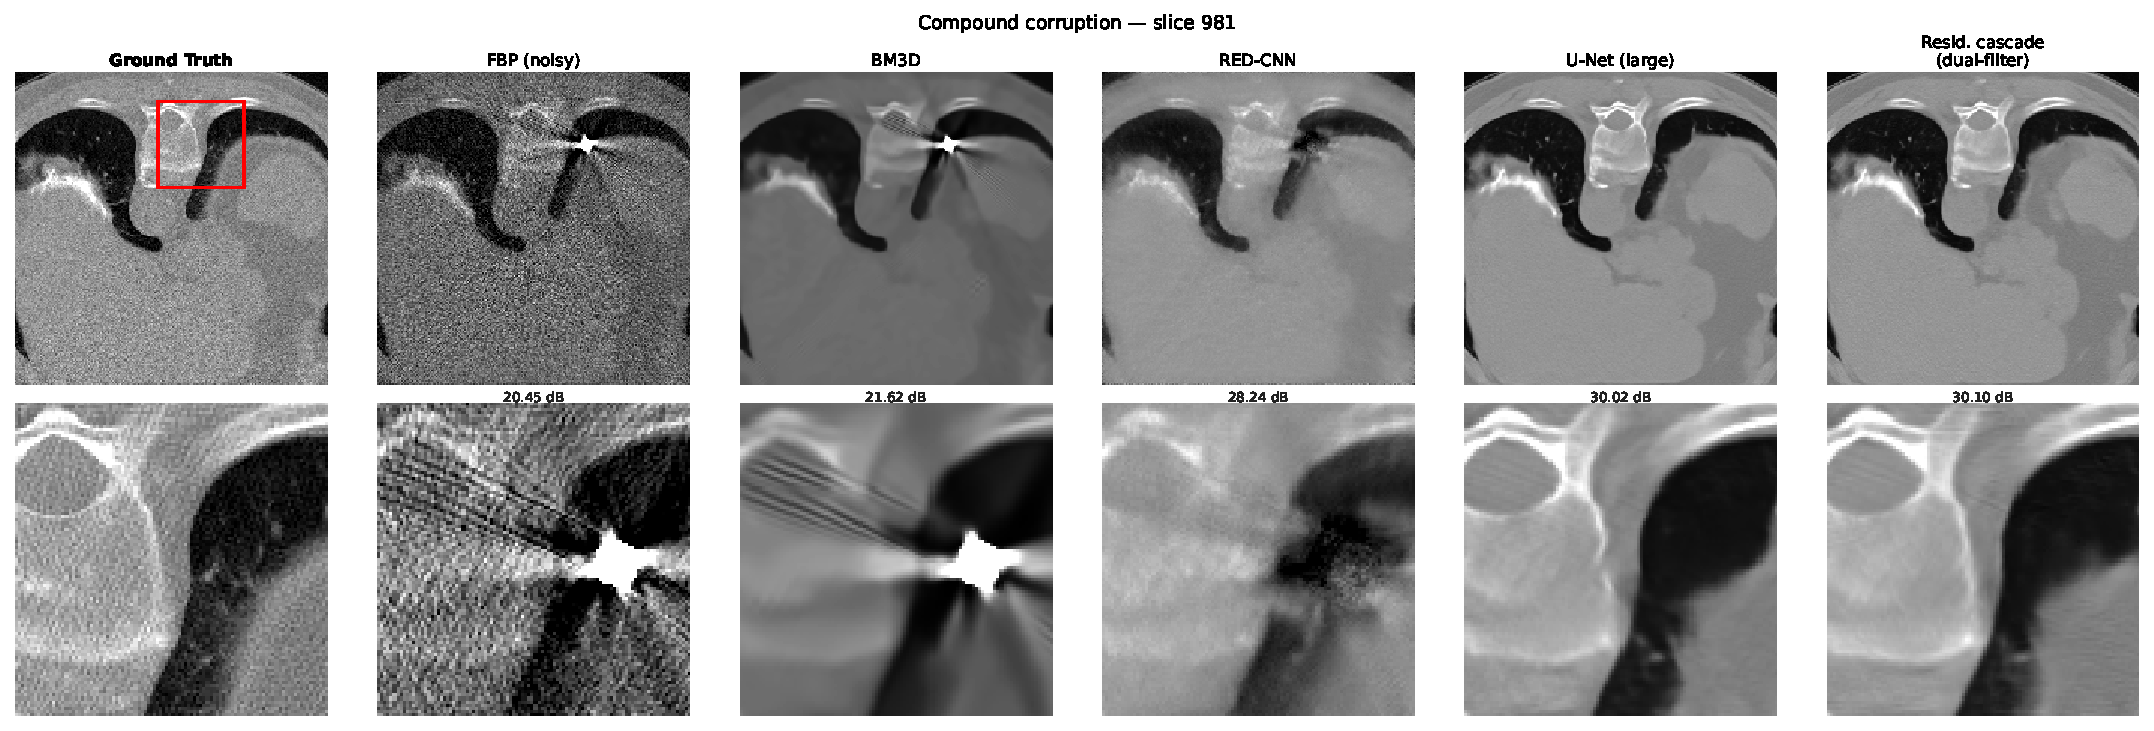
\includegraphics[width=\linewidth]{figures/results/fig_app_metal_slice0981.pdf}
    \caption[Slice~981: metal artifact condition.]{%
        Slice~981 with added metal implant artifacts (1--2 implants, effective
        attenuation scale 0.10--0.30, photon-starvation clipping active). Bright
        and dark saturation streaks are prominent in the FBP reconstruction. The
        residual dual-filter cascade achieves the strongest streak suppression
        among all methods, most clearly visible in the zoomed crop.
        RED-CNN reduces diffuse noise but leaves the highest-saturation streak
        regions largely unresolved.}
    \label{fig:app_qual_metal_981}
\end{figure}

\begin{figure}[!htbp]
    \centering
    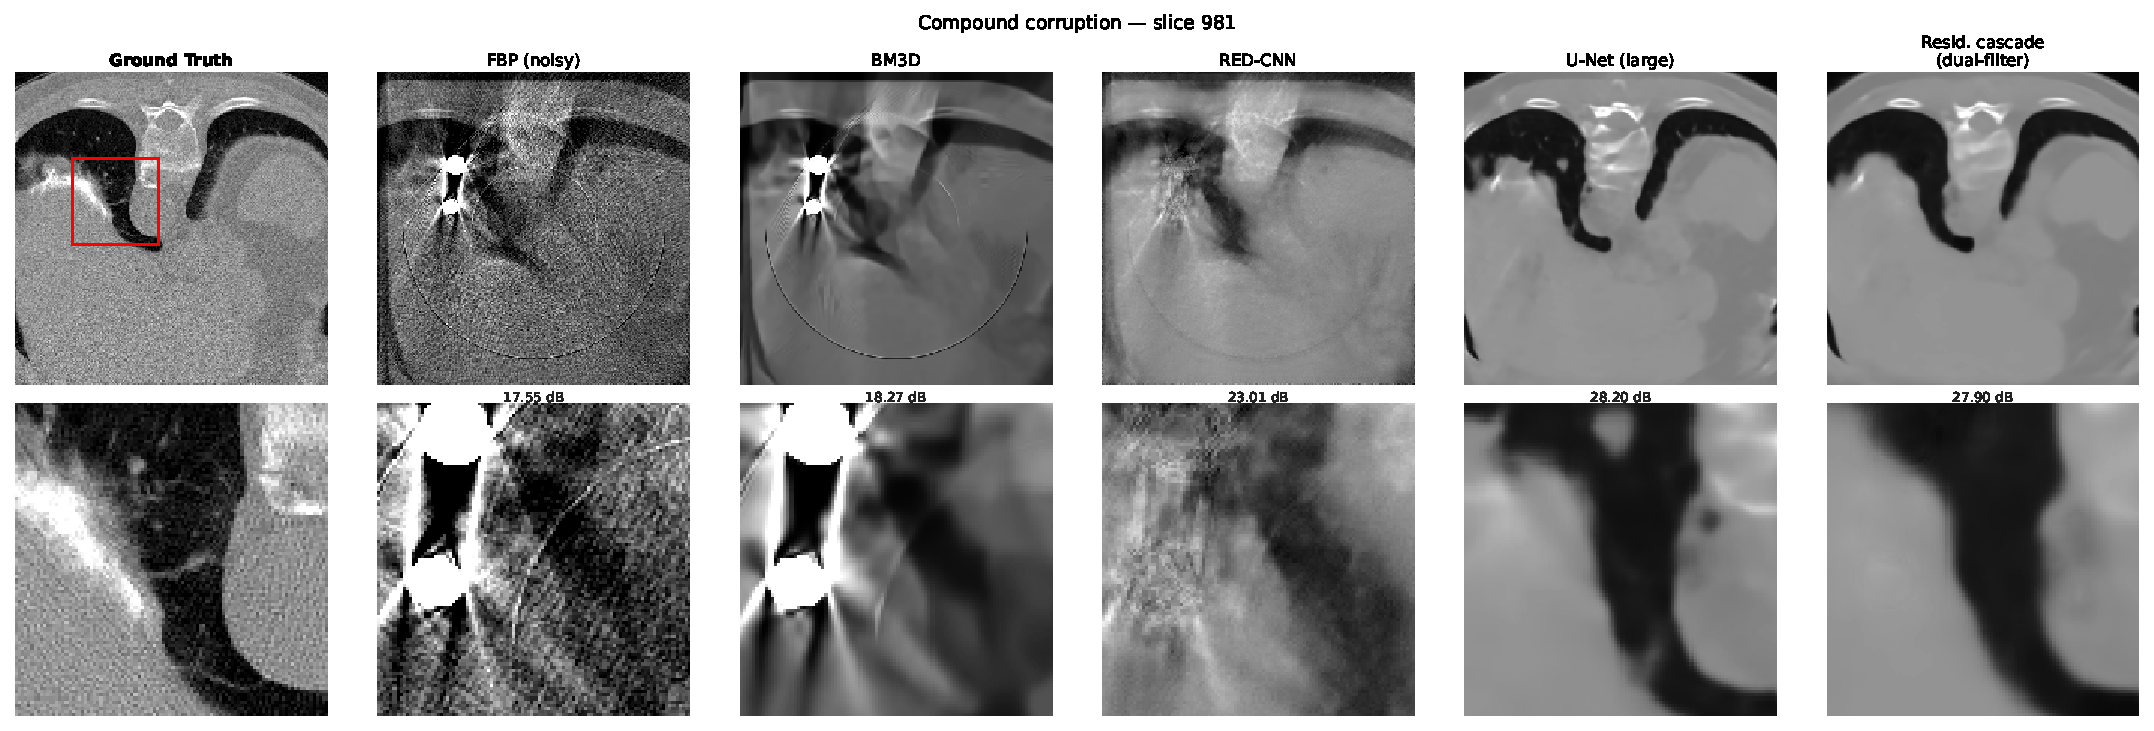
\includegraphics[width=\linewidth]{figures/results/fig_app_compound_slice0981.pdf}
    \caption[Slice~981: compound corruption condition.]{%
        Slice~981 under compound corruption (Poisson noise, motion, ring, and
        metal artifacts co-occurring simultaneously). This is the hardest
        corruption regime evaluated in this thesis. Both learned U-Net models
        substantially suppress the combined degradation, while BM3D and RED-CNN
        leave visible structured artifact residuals. The residual dual-filter
        cascade provides the most complete restoration in the zoomed crop, consistent
        with the quantitative results in \Cref{tab:exp_cascade}.}
    \label{fig:app_qual_compound_981}
\end{figure}

The per-artifact-count PSNR breakdown for all evaluated methods is reported in \Cref{tab:exp_per_artifact} in \Cref{chap:experiments}.


%%─────────────────────────────────────────────────────────
\chapter{Implementation Details and Hyperparameters}
\label{app:implementation}

\section*{Training hyperparameters}

\Cref{tab:app_hyperparams} provides the complete hyperparameter specification used for all models in this thesis. Hyperparameters shared across all cascade variants are listed in the upper block; model-specific settings are listed in the lower block.

\begin{table}[!htb]
    \centering
    \caption[Complete training hyperparameters.]{%
        Training hyperparameters shared across all model variants unless otherwise noted.}
    \label{tab:app_hyperparams}
    \setlength{\tabcolsep}{5pt}
    \small
    \begin{tabular}{@{}lll@{}}
        \toprule
        Hyperparameter & Value & Notes \\
        \midrule
        \multicolumn{3}{l}{\textit{Optimiser}} \\
        Algorithm       & AdamW & \\
        Learning rate   & $3\times10^{-4}$ & $1\times10^{-4}$ for RED-CNN \\
        $(\beta_1,\beta_2)$ & $(0.9,\,0.999)$ & \\
        Weight decay    & $10^{-2}$ & \\
        \midrule
        \multicolumn{3}{l}{\textit{Training schedule}} \\
        Epochs          & 150 (max) & early stopping, patience 15 \\
        Batch size      & 4 slices & \\
        Checkpoint selection & lowest validation loss & \\
        \midrule
        \multicolumn{3}{l}{\textit{Data}} \\
        Dataset         & LoDoPaB-CT~\cite{Leuschner2021} & \\
        Train / val / test split & 35\,820 / 3\,522 / 3\,553 & official split \\
        Corruption (train) & stochastic per epoch & fresh draw each epoch \\
        Corruption (val/test) & seeded: \texttt{seed\,+\,idx} & deterministic \\
        \midrule
        \multicolumn{3}{l}{\textit{Architecture (single-stage U-Net small)}} \\
        Encoder widths  & $[32,64,128,256]$ & \\
        Downsampling levels & 3 & $2\times2$ max-pool \\
        Upsampling      & bilinear + concat skip & \\
        Normalisation   & GroupNorm (8 groups) & \\
        Output activation & sigmoid & \\
        Parameters      & \num{1798113} & \\
        \midrule
        \multicolumn{3}{l}{\textit{Architecture (single-stage U-Net large)}} \\
        Encoder widths  & $[64,128,256,512]$ & \\
        Parameters      & \num{7184321} & \\
        \midrule
        \multicolumn{3}{l}{\textit{Loss weights}} \\
        Stage~1 loss    & $0.5\,\mathcal{L}_\mathrm{SSIM} + 0.5\,\mathcal{L}_1$ & \\
        Naive Stage~2 loss & $0.5\,\mathcal{L}_\mathrm{SSIM} + 0.5\,\mathcal{L}_1$ & \\
        Residual Stage~2 loss & $0.4\,\mathcal{L}_1(\hat{\mathbf{r}}) + 0.3\,\mathcal{L}_\mathrm{SSIM} + 0.3\,\mathcal{L}_\nabla$ & \\
        Cascade joint weight & $w_1=w_2=0.5$ & end-to-end only \\
        \midrule
        \multicolumn{3}{l}{\textit{Hardware}} \\
        GPU             & single NVIDIA GPU & \\
        Framework       & PyTorch & \\
        \bottomrule
    \end{tabular}
\end{table}

\section*{Code availability}

The full implementation, including the corruption pipeline, model definitions, training scripts, and evaluation notebooks, is available at \url{https://github.com/Mohammad-Shiblu/ct-restoration-cascade}. All seeded corruption draws and checkpoint files are included to allow exact reproduction of the reported results.


%%─────────────────────────────────────────────────────────
\chapter{Corruption Protocol Parameter Tables}
\label{app:protocol_params}

The corruption protocol is fully specified in \Cref{sec:meth_compound}. For convenience, \Cref{tab:app_motion_params,tab:app_ring_params,tab:app_metal_params,tab:app_compound_probs} reproduce the parameter tables from \Cref{chap:methodology} and add the compound activation statistics in one place.

\begin{table}[!htb]
    \centering
    \caption[Motion artifact parameters (reproduced from \Cref{tab:meth_motion_params}).]{%
        Sampling ranges for the motion artifact model. See \Cref{sec:meth_motion} for derivation.}
    \label{tab:app_motion_params}
    \begin{tabular}{llll}
        \toprule
        Parameter & Symbol & Range & Physical interpretation \\
        \midrule
        Peak detector shift     & $A$            & $[10,20]$ bins & $\approx7$--$14\,\text{mm}$ motion \\
        Breathing cycles / scan & $f$            & $[0.5,1.5]$    & quasi-periodic respiration \\
        Initial phase           & $\varphi$      & $[0,2\pi)$     & random scan-start phase \\
        Activation probability  & $p_\text{mot}$ & $0.5$          & \\
        \bottomrule
    \end{tabular}
\end{table}

\begin{table}[!htb]
    \centering
    \caption[Ring artifact parameters (reproduced from \Cref{tab:meth_ring_params}).]{%
        Sampling ranges for the ring artifact model. See \Cref{sec:meth_ring} for derivation.}
    \label{tab:app_ring_params}
    \begin{tabular}{llll}
        \toprule
        Parameter & Symbol & Range & Physical interpretation \\
        \midrule
        Affected columns        & $|\mathcal{C}|$ & $\{1,\dots,5\}$  & sparse detector faults \\
        Detector gain           & $g_c$           & $[0.5,0.95]$     & $5$--$50\,\%$ calibration error \\
        Implied offset          & $|c_c|$         & $[6.3\times10^{-4},8.5\times10^{-3}]$ & $\mu_{\max}$-normalized \\
        Activation probability  & $p_\text{ring}$ & $0.5$            & \\
        \bottomrule
    \end{tabular}
\end{table}

\begin{table}[!htb]
    \centering
    \caption[Metal artifact parameters (reproduced from \Cref{tab:meth_metal_params}).]{%
        Sampling ranges for the metal artifact model. See \Cref{sec:meth_metal} for derivation.}
    \label{tab:app_metal_params}
    \setlength{\tabcolsep}{4pt}
    \small
    \begin{tabular}{@{}llll@{}}
        \toprule
        Parameter & Symbol & Range & Physical interpretation \\
        \midrule
        Number of implants      & $N_\mathrm{impl}$  & $\{1,2\}$           & \\
        Mask radius             & $r_\mathrm{impl}$  & $[3,12]\,\text{px}$ & $\approx2$--$9\,\text{mm}$ \\
        Metal strength          & $\alpha$           & $[0.10,0.30]$       & effective attenuation \\
        Radial position         & $r/H$              & $[0.05,0.35]$       & inside FOV \\
        Activation probability  & $p_\mathrm{metal}$ & $0.3$               & \\
        \bottomrule
    \end{tabular}
\end{table}

\begin{table}[!htb]
    \centering
    \caption[Expected compound artifact distribution.]{%
        Expected fraction of training samples carrying each artifact count, derived analytically
        from the independent Bernoulli gates with
        $(p_\mathrm{mot}, p_\mathrm{ring}, p_\mathrm{metal}) = (0.5, 0.5, 0.3)$.}
    \label{tab:app_compound_probs}
    \begin{tabular}{lc}
        \toprule
        Number of additional physical artifacts & Expected fraction \\
        \midrule
        0 (noise only)  & $17.5\,\%$ \\
        1               & $42.5\,\%$ \\
        2               & $32.5\,\%$ \\
        3               & $7.5\,\%$  \\
        \bottomrule
    \end{tabular}
\end{table}
           % Appendix A/B/C
\cleardoublepage

%% Do not change, auto-generated lists of figures, tables and literature %%
% Glossar
\printunsrtglossary[type=abbreviations]
\cleardoublepage

% List of figures
\addcontentsline{toc}{chapter}{\listfigurename}
\listoffigures
\cleardoublepage

% List of tables
\addcontentsline{toc}{chapter}{\listtablename}
\listoftables
\cleardoublepage

% Literature list
% %CONFIG:
%\selectlanguage{german}{\addcontentsline{toc}{chapter}{\bibname}}
\selectlanguage{english}{\addcontentsline{toc}{chapter}{\bibname}}

\printbibliography
\end{document}
